\documentclass[10pt]{reportMaster}

%%%%%%%%%%%%
% switches %
%%%%%%%%%%%%
% Define the switch using "\newif\ifNAME", where the name of the switch is "NAME"
%%
\newif\ifMonochrome
\newif\ifThousandsComma
%%
% By default, all switches are 'false'. Use "\NAMEtrue" to set "NAME" to 'true'.
% Uncomment lines below to toggle switches on:
%%
%
% Sets the document to a monochrome version that is better to print in black-and-white
%%%%%%%%%%%%
\Monochrometrue
\ThousandsCommatrue
%
%%%%%%%%%%%%

\usepackage[a4paper]{geometry}
\usepackage{subcaption}
\usepackage{placeins}
\usepackage{amsmath,amssymb}
\usepackage{mathtools}
\usepackage{algorithm}
\usepackage[noend]{algpseudocode}
\usepackage{refcount}
\usepackage{scrextend}
\usepackage{doi}
\renewcommand{\doitext}{}
\usepackage{apacite}
\usepackage[table]{xcolor}
\usepackage{cleveref}
\usepackage{multirow}
\usepackage{changepage}
% \usepackage{tabularray}
% \usepackage[table]{xcolor}

%%
% Use commands to imitate behaviour from book class, 
%  which cannot be used due to 'reportMaster' being 
%  a type of "report" document.
% Found at: https://tex.stackexchange.com/a/154666
%%
\newcommand\frontmatter{%
    \cleardoublepage
  \pagenumbering{roman}}

\newcommand\mainmatter{%
    \cleardoublepage
  \pagenumbering{arabic}}

% Command for thousands separator
\ifThousandsComma
  \newcommand{\thsep}{,}
\else
  \newcommand{\thsep}{\,}
\fi


\makeatletter
%%
% Use modified titlepage environment to NOT reset
%  page numbering when inside the titlepage and abstract
% Found at: https://tex.stackexchange.com/a/172005
%%
\renewenvironment{titlepage}
 {
  \if@twocolumn
    \@restonecoltrue\onecolumn
  \else
    \@restonecolfalse\newpage
  \fi
  \thispagestyle{empty}
 }
 {
  \if@restonecol
    \twocolumn
  \else
    \newpage
  \fi
 }
% %
% Use modified command to fix hyperref linking to 
%  the wrong algorithm for pseudocode line labels.
% Found at: https://tex.stackexchange.com/a/148977
%%
\providecommand\theHALG@line{\thealgorithm.\arabic{ALG@line}}
\makeatother

%%% The title of the thesis, and the author (student) of the thesis
\title{Memory Efficient B*}
\author{Pascal R. Anema}

%%% Uncomment the line with the Master program of the student
% \nameMastersProgramme{Data Science for Decision Making}  
\nameMastersProgramme{Artificial Intelligence}

%%% Here, write the department supervisor(s), as well as all department examiners; 
%%% Write also any external supervisor(s), if applicable
\committee{Prof. Dr. Mark H. M. Winands \\ Dr. Dennis J. N. J. Soemers}
\date{\today}

\begin{document}

\frontmatter
\maketitle

%%%% PREFACE %%%%
\chapter*{Preface}
\addcontentsline{toc}{chapter}{Preface}
\thispagestyle{empty}
%
%
%
This thesis builds directly on the work from a research internship report \cite{Anema2025}, which was written under the supervision of Prof. Dr. Mark H.M. Winands and Dr. Dennis J.N.J. Soemers and was submitted on 27 February 2025. The initial goal of that report was to achieve a result now presented in this thesis: a description of the depth-first B* variant df-B*. However, this thesis would not have been the same without the advances in artificial game trees developed during the internship report.

The process of writing this thesis has been an exercise in limiting my creativity. Developing the algorithms and conducting the experiments was engaging and exciting, but the task of documenting the work proved challenging at times. I would like to thank several people for supporting me throughout this process, in particular by providing the encouragement needed to prioritise writing over implementing further algorithms.

I would like to express my gratitude to Prof. Mark H.M. Winands for his supervision and guidance throughout both the internship and this thesis. I want to thank my parents and my siblings for their support in various forms, and my dearest friend for her unwavering support and understanding.
\\\phantom{}\vspace{1ex}\\
\noindent I wish you a pleasant reading of this thesis.

%%%% Abstract %%%%
\begin{abstract}
\addcontentsline{toc}{chapter}{Abstract}
    Artificial Intelligence (AI) techniques in games have been developed for decades, progressing the field of computer-aided decision-making with them. Game tree search is a particular branch of game AI. This discipline represents the game as a rooted tree, for which the best node at its root is the next move to play. B* is a best-first game-tree search technique developed in the late 1970s, which was later used for competitive endgame play of Scrabble in the 2000s. B* is unique in its construction and capabilities, but has not been extensively researched in the last two decades. A recent report has shown that B* can solve large problems more efficiently than was previously known. However, B* is limited in the size of problems it can solve, due to its memory requirements. In this thesis, we address this problem by introducing two B* variants: the memory-efficient multi-level B*² and the memory-independent depth-first df-B*. 
Experimental evaluation on over 37,000 artificial game trees showed B*² requires just 7.6 times the square root of the memory usage of B*. Whereas the experiments showed that df-B* only requires a near-constant amount of memory, effectively never running out of memory on any problem. However, we observed that df-B* has significantly reduced computational efficiency by approximately a factor of 22 to 23 compared to B*. By contrast, we found B*² was able to solve some problems more efficiently than B*, and was, on average, only a factor of up to 3 times less computationally efficient. In conclusion, B*² was found to be effective for search on large problems, whereas df-B* was found to be effective for search on very large problems, being effectively unrestrained by memory limitations. These results were found to align with existing research on memory-efficient variants of the best-first game-tree solver Proof-Number Search.
\\
\phantom{}
\vspace{2ex}\\
\textbf{Keywords:} B* Search $\cdot$ Artificial Game Trees $\cdot$  Depth-First Search $\cdot$ Adversarial Search $\cdot$ Artificial Intelligence
\end{abstract}

\newpage
\addcontentsline{toc}{chapter}{Contents}
\tableofcontents

%%%% Article %%%%
\mainmatter
%
%
%       %%%%%%%%%%%%%%%%%%%%%%%%%%%%%%%%%%%%%%%%%%%%%%%%%
%       % TODO:                                         %
%       % * afkortingen (AFK) fixen:                    %
%       %   - vraag aan Mark de specifieken             %
%       %   - (?) in elk hoofdstuk opnieuw uitleggen    %
%       % * referencies fixen:                          %
%       %   - vraag aan Mark de specifieken             %
%       %   - (?) in elke alinea opnieuw refereren      %
%       %%%%%%%%%%%%%%%%%%%%%%%%%%%%%%%%%%%%%%%%%%%%%%%%%
%
%
\chapter{Introduction}
This thesis covers the topic of game-playing Artificial Intelligence (AI) systems referred to as game-tree search techniques. We focus specifically on a game-solving technique called B* \cite{Berliner1979}, which efficiently proves the best moves in a game, but may use much memory to do so. This thesis addresses the memory problem of B* by introducing two new variants called ${\text{B*}}^2$ and df-B*. This chapter introduces the main topics discussed in this thesis and is structured as follows.

Section \ref{sec:introAIandGames} introduces the topic of games as an environment for AI research and provides a relevant history of the field. Section \ref{sec:introGameTreeSearch} introduces game-tree search techniques and much of the search-related terminology used throughout this thesis. Section \ref{sec:introGameSolvers} introduces the specific category of game-tree search techniques we focus on in this thesis: game solvers, and provides an introductory explanation of B* and two other game-solving techniques. Section \ref{sec:problemStatementAndRQs} provides the problem statement and research questions of this thesis. Finally, the overall outline of this thesis is provided in Section \ref{sec:outline}.

\section{Artificial Intelligence and Games}
\label{sec:introAIandGames}
Games have been at the forefront of Artificial Intelligence (AI) development for decades, and they continue to serve as a testing ground for new developments. 
Games like Chess, Settlers of Catan, Risk, Go, and many video games provide predictable environments on which AI agents can easily be trained, tested, and evaluated. Board games are simple to model, compared to real-world problems, with predefined rules and full knowledge of probability distributions, such as possible draws from a deck of cards or possible outcomes from a dice roll. In games, there is seldom a mismatch between the model the agent learns to play in and the environment, which is the game itself. Such that the only complexity is in designing the algorithm for playing the game itself. Video games may not always be easy to model, but the game itself is usually directly accessible, and its use does not bear many costs. So AI agents for video games can often be trained, tested, and evaluated directly in the game environment itself, which simplifies the development process and reduces costs. Finally, evaluation of agents, through the use of benchmarks, is generally simple in game environments. Single-player games and puzzles can simply be played to evaluate an agent’s performance, whereas competitive games allow competitions with other AI agents or human players to be used as benchmarks.

Progress in game AI has been significant in the last 50 years. Whenever an AI agent defeats expert human players in a game for the first time, it marks an important milestone. Fairly cemented in the general consciousness is the computer players’ supremacy in the game of Chess. This may have started in 1997, when IBM’s Chess program \textsc{DeepBlue} \cite{Campbell2002} was able to beat the strongest Chess player at the time, Gary Kasparov, in 1997 using $\alpha\beta$ search and dedicated hardware. In Backgammon, master-level play was attained in 1994 by the reinforcement learning neural network agent \textsc{TD-Gammon} \cite{Tesauro1994}, which was developed throughout the 1990s. In 1998, \textsc{TD-Gammon} was defeated by the Backgammon world champion with a margin of 8 points over 100 games \cite{Tesauro2010}. In 1995, the parallel $\alpha\beta$-search driven Checkers program \textsc{Chinook} \cite{Schaeffer1992, Schaeffer1996} halted competing against humans in tournaments and instead started work on a different task: solving the game of Checkers. 
The team behind \textsc{Chinook} succeeded in this in 2007 \cite{Schaeffer2007}, proving that perfect play of Checkers from the starting position leads to a draw, a draw that \textsc{Chinook} can guarantee through play against any possible counter strategy: the holy grail of game AI research.
For a long time, it seemed that the game of Go was resistant to the conquest of AI techniques in games, so much so that when \textsc{AlphaGo} \cite{Silver2016} defeated one of the strongest Go players in the world, Lee Sedol, by 4 games to 1 in 2016, it seemed to come out of nowhere for many. The Monte-Carlo Tree Search (MCTS) \cite{Coulom2007} based program, guided by two large deep neural networks (DNNs), was initially trained on expert human players’ games of Go. However, it achieved even better play as \textsc{AlphaGo Zero} \cite{Silver2017} in 2017, which learnt entirely from self-play and had no initial knowledge of the game beyond its rules. The techniques developed for game-playing agents have advanced greatly throughout the decades, but they have also been applied to %many 
other fields beyond games, such as to chemical synthesis \cite{HeifetsJurisica2012, Franz2022}. % TODO add some references for other fields

\section{Search and Games}
\label{sec:introGameTreeSearch}
In this thesis, specific techniques of game AI research will be discussed, called tree search techniques. The previously mentioned programs \textsc{DeepBlue}, \textsc{Chinook}, and \textsc{AlphaGo} are all tree search techniques, which may utilise other techniques as well, like machine learning for \textsc{AlphaGo}, which was the main kind of method used in \textsc{TD-Gammon}.

The `tree’ that is being searched in tree search techniques is called the game tree, which is a tree formed from the current and future possible states of the game. Looking at the game board, a game state is a frozen snapshot of all the information about the game that changes throughout the game and may affect the decisions players can make and the outcomes they have. Typically, we define a node in the game tree to be any such state where the `current player’ gets to make a decision, which determines the next state of the game. All possible decisions this player can make are their available moves, and all the nodes following each of these moves are the so-called children of that node. Nodes, or game states, are also often called game positions, which refers to the position of all the pieces on the board.

Eventually, throughout the play of the game, a position may be reached where the game is terminated, such as when it is won, lost, or tied. This is referred to as a terminal position, and the nodes representing these positions are called leaf nodes. Any other nodes are internal nodes: positions where the game is still going on. Leaf nodes may be given a value based on which player won the game, or based on what score each of the players received. This value may be relayed back to its parent node, the single node whose children include this one. For example, if all possible moves from the parent lead to a win for player 1, then this parent node has the same value as the leaf nodes at these win positions. This can be extended to assign a value to each internal node of the tree, based on all possible game states that follow from it. If we assume that all players play the game optimally, meaning they attempt to maximise their own score with full knowledge of the game, then the value we assign to these nodes is called the game-theoretical value. In two-player zero-sum games where a win for one player determines a loss for the other, we can keep track of just one value at each node. One player tries to maximise this value, while the other player tries to minimise it. Hence, this is referred to as the minimax value of the sub-tree originating at that node.

If the true minimax values of the children of a node are known, you can essentially play the optimal next move at that node. However, the search tree of a game may often be much too large to search exhaustively, so intelligent techniques are needed to make the best possible estimate. This may include estimating the minimax value at internal nodes, known as internal node evaluation, and skipping the search of certain nodes, referred to as pruning. Many tree search techniques aim to estimate the minimax value of the current game position’s node (the root node), like MCTS \cite{Coulom2007} and $\alpha\beta$ search \cite{Knuth1975}. This can be achieved through simulated games originating at some position, as in the case of MCTS, where the average number of wins or losses in simulation determines the estimated value of a node. Nodes are also often evaluated using game-specific knowledge to assign some value to the game positions; the function that assigns these values is called a heuristic evaluation function. Heuristic evaluation functions may also be combined with MCTS, as is done for \textsc{AlphaGo} \cite{Silver2016}, where a neural network operates as a node evaluation function.

To determine the best move at the root, search is required: we need to traverse the tree by iteratively choosing which nodes to check next and incorporating what we learned into our final answer. This is what search is all about: what node to select next? When a node is selected, it is `expanded’, which means that we check for all the possible moves from that node and consider the resulting child nodes. Depth-first search selects one of the children of the current node to be expanded next, and then continues recursively, going deeper and deeper into the tree. Depth limits and the pruning of child nodes deemed `irrelevant’ for the current search ensure that the algorithm terminates on time. The benefit of depth-first search is that it is not constrained by the memory limits of computers. The performance of these algorithms can depend strongly on the order in which moves are considered, which is known as the move ordering. Another method is to search in a best-first manner, which often keeps the entire tree in memory, but selects the next node to be the `best’ node to expand next. This is typically a node chosen to optimise for the most `progress' made per expansion, referred to as the most-informative, most-promising, or most-proving node. The benefit here may be a reduction in the total number of nodes searched. However, the memory limits may restrict the expanse of the search greatly compared to other methods. After selecting a node, its children are usually evaluated, and the information may be used to further advance the search and eventually determine the value of the children of the root node, which usually decides which move the agent plays.

However, the minimax value is not the only quantity that tree search techniques may aim to evaluate. The next section covers a special subclass of search techniques that do not aim to estimate values, but instead aim to prove specific quantities or qualities of game positions. 


\section{Adversarial Game Solvers}
\label{sec:introGameSolvers}
% Where an adversarial game-playing agent may use any assumptions about the game to decide its next move, a specific kind of agent ...
An important detail about value estimation techniques, as they are described above, is that they may not necessarily guarantee that the best move is selected. The process of estimating minimax values and pruning positions with unfeasibly high or low scores depends highly on the maximum depth searched and the `correctness’ of the evaluation function. Methods have been developed to counteract this, and one of them is the class of methods here called game solvers. If searched deep enough, specialised techniques can prove a win, draw, or loss at game positions more effectively than value estimation, and they can prove other objectives as well. These techniques use evaluation functions, move orderings, and pruning procedures which are designed to provide a proof for whatever quantity is being tested while searching as few nodes as possible. For example, Proof-Number Search can be used to evaluate which moves could lead to a proven check in Chess, which is a useful game-specific quality of game positions in Chess. Additionally, game solvers are often used to solve puzzles, with or without an opponent. The following subsections cover three of these game-solving techniques: Proof-Number Search (\ref{subsec:introPNS}), $\lambda$-Search (\ref{subsec:lambdaSearch}), and B* (\ref{subsec:introBstar}).

\subsection{Proof-Number Search}
\label{subsec:introPNS}
Proof-Number Search (PNS) \cite{Allis1994} is a technique used to prove binary statements about nodes in an adversarial game tree. This is typically applied to binary statements that can be determined from the sub-tree of a node or just the node itself for terminal nodes. So the statement ``this node achieves a higher value than the alternatives’’ would not work for PNS, because it requires more information than what can be obtained from the sub-tree alone. Binary qualities like the existence of impasses, checks, wins, draws, or losses for the entire game or for a sub-problem of the game can be evaluated using PNS. A single PNS tree usually solves just a single binary question at a time, but multiple trees could be used to evaluate more complicated or categorical quantities.

PNS works by building a game tree, like other best-first techniques, containing proof-numbers and disproof-numbers for each node. Proof-numbers essentially count the minimum number of nodes that need to be evaluated as true (proven) in a node’s sub-tree to evaluate whether its statement is true. Similarly, disproof-numbers count the minimum number of nodes in the sub-tree that need to be evaluated as false (disproven) to evaluate the node as false. At each step, the best node is selected to be expanded next, which is the `most-proving node’: the node with the adversarially decided highest chance to advance the proof. Search is terminated when the root node is proven or disproven.

PNS is effective and popular for solving games, as it was developed for this purpose \cite{Allis1994}. PNS and its variants are effectively used to help prove games or strengthen game-playing agents in various domains \cite{Winands2012}, including Shogi \cite{Seo2001}, Othello \cite{Nagai2002}, Lines of Action \cite{Winands2004}, Go \cite{Kishimoto2005b}, and Connect6 \cite{Xu2009, Wu2011}. The previously mentioned Checkers solver \textsc{Chinook} \cite{Schaeffer2007} also uses depth-first Proof-Number Search (df-PN) \cite{Nagai2002} when an $\alpha\beta$ search could not find a proven result in time. PNS and df-PN have also been applied to the fields of chemical (retro-)synthesis \cite{HeifetsJurisica2012, Franz2022}.

\subsection{\texorpdfstring{$\lambda$}{λ}-Search}
\label{subsec:lambdaSearch}
$\lambda$-Search \cite{Thomsen2000} is a depth-first technique for proving the existence of a forced sequence of moves that achieves a tactical goal in adversarial zero-sum games. Unlike PNS \cite{Allis1994}, $\lambda$-search does not solve arbitrary binary goals. It is designed for goals that form a threat to the opponent, typically requiring a response, and provide a tactical advantage towards winning the game. A goal can be the win condition itself, such as a forced checkmate in Chess, or a tactical gain such as capturing a large territory in Go.

$\lambda$-Search iteratively builds higher hierarchies of so-called $\lambda$-trees. A $\lambda^1$-tree represents a forced threat sequence towards the goal, while a $\lambda^2$-tree represents a threat sequence towards a $\lambda^1$-tree, and so on for higher orders of $\lambda^n$-trees. This structure relies on the null-moves assumption: the goal is guaranteed if the opponent passes their turn $n$ times at a $\lambda^n$-node. Passing could also mean the opponent plays a move outside the $\lambda^n$-tree, as these trees contain only moves that belong to the relevant threat sequences. This can greatly reduce the branching factor of the search and makes the search more focused in games with many possible moves.

This technique may be applied to Chess or Go, but any game with threat sequences may work, as 4x4 tic-tac-toe was also provided as an example by \citeA{Thomsen2001}. $\lambda$-Search has since been used as a basis for other proof-search methods, such as RZOP \cite{Wu2010} for Connect6. One difficulty noted by Thomsen is the possibility of inversions, where the opponent can turn a threat sequence into a counter-attack to escape the threat rather than defending against it. Thomsen outlined a possible direction for handling this issue, but the general problem remains open and has not been resolved in later work, such as RZOP.

\subsection{B* Search}
\label{subsec:introBstar}
The technique of B* \cite{Berliner1979} was developed to prove the optimal next move in games through the use of an evaluation function which provides a lower and upper bound on the true minimax value of the tree. Rather than proving a binary quality of the game state, B* maintains bounds on the minimax value for all nodes in its saved search tree. Updating these bounds eventually leads to the stop condition of B*: separation. Contrary to value estimation techniques, B* terminates consistently when the best move has been proven and no later, as that is when one move has a lower bound greater than any upper bound of the alternative moves. Value estimation guarantees selection of the best move only if the evaluation function is itself perfect, which would make the search unnecessary. B*, on the other hand, will always terminate with the best move if the provided bounds accurately contain the minimax value, which is a looser requirement than an exact match of the minimax value. In practice, however, the evaluation function might not be correct, in which case B* cannot guarantee the best move: the guarantees depend on the evaluation function, unlike Proof-Number Search, which is always correct for binary qualities of the game-state.

However, B* differs not only from value estimation in the use of bounds on the minimax value. It additionally employs two separate strategies for completing the proof. When the search is not confident about the currently most optimistic move, it expands its sub-tree further to improve its lower bound. When the confidence is increased, the program may choose one of two separate strategies: Prove-Best, or Disprove-Rest. Either we attempt to raise the lower bound further: Prove-Best; or we attempt to lower the upper bounds of the alternatives: Disprove-Rest. Either strategy may lead to the completion of the proof, but the strength of B* lies mainly in the conjunction of these two strategies. It is in a unique position as a game solver that utilises heuristics to estimate the game-theoretical value, which could skip major parts of the search that exact solvers may not be able to skip while remaining prudent.

Early research, like \citeA{Palay1982} and \citeA{Berliner1996}, presented promise for B* in the game of Chess. However, not much research was published after this, possibly due to the greater promise of depth-first value estimation methods. These can be pushed to further limits with specialised hardware, as shown by \citeA{Campbell2002}, which proved successful in the game of Chess. However, B* is a best-first search technique, which requires the game tree to be stored in memory. For small proofs, this is not a problem, and it does not hinder B* from performing well in certain domains, such as in the end-game play of Scrabble \cite{Sheppard2002}. But for much larger proofs, sub-trees may grow to sizes too large to store in memory, which currently cannot be solved with B* alone.

A recent report by \citeA{Anema2025} continues research on B* with the introduction of the Disprove-Best variant of B*, which improves the performance of B* on the specific sub-problem of lowering the upper bound of `false’ best moves. Furthermore, the report also re-evaluates the performance of B* on large artificial game trees, which shows that the efficiency of B* grows further as the size of the problem increases. This is promising, as it shows that B* could perform well on large problems if memory allows it. As such, the report advises future research to focus on modifying B* to work on larger problems.

A similar task has been executed for the previously mentioned best-first Proof-Number Search \cite{Allis1994}. The ${\text{PN}}^2$ \cite{Breuker1998} and df-PN \cite{Nagai2002} algorithms expand Proof-Number Search to multi-level search and depth-first search, respectively, both of which allow PNS to search much larger problems. This thesis thus aims to apply a similar improvement to B*: expanding B* to work on larger trees.

\section{Problem Statement and Research Questions}
\label{sec:problemStatementAndRQs}
We have established that B* is a unique heuristic search technique that is also a game solver, with specialised strategies for proving the optimal move. One of its major drawbacks is the limit of memory usage due to its reliance on a stored game tree for best-first search. B* has been shown to work well on larger problems, so this problem is interesting to solve. The same has challenged the best-first game solver PNS before, which prompted research into depth-first and multi-level variants, some of which are still ongoing research.
Therefore, the \textbf{problem statement} of this thesis is:
\\[1\baselineskip]
\textit{How can B* be extended to search on much larger problems?}
\\[1\baselineskip]
To address this problem statement, we introduce two novel B* variants inspired by the PNS variants ${\text{PN}}^2$ \cite{Breuker1998} and df-PN \cite{Nagai2002}. The multi-level variant ${\text{B*}}^2$, generalised to ${\text{B*}}^k$, reduces memory usage by keeping a smaller game tree in memory. The depth-first variant df-B* limits the memory footprint of B* to a fixed-size transposition table.
This leads to the following three \textbf{research questions}:
\begin{enumerate} % TODO rewrite RQs:
    % \item \textit{How can we transfer B* to Multi-Level search?}
    % \item \textit{How and when should we stop the multi-level search?}
    % \item \textit{How can B* be formulated as a depth-first search?}
    % \item \textit{How do different B* variants behave with multi-level search?}
    % NEW RESEARCH QUESTIONS: (are these better? are these good enough?)
    \item \textit{How can B* be adapted to multi-level (${\text{B*}}^{\text{\hspace{1pt}}\textit{2}}$) or depth-first (df-B*) search?}
    \item \textit{How do ${\text{B*}}^{\text{\hspace{1pt}}\textit{2}}$ and df-B* affect the memory usage of search compared to B*?}
    \item \textit{How do ${\text{B*}}^{\text{\hspace{1pt}}\textit{2}}$ and df-B* compare to B* in terms of computational efficiency?}
    % \item \textit{How does the choice of program parameters affect the memory usage and computational efficiency of ${\text{B*}}^{\text{\hspace{1pt}}\textit{2}}$ and df-B*?}
    % \item \textit{How does the memory usage of ${\text{B*}}^{\text{\hspace{1pt}}\textit{2}}$ and df-B* compare to that of B*?}
    % \item \textit{How do the number of expansions, evaluations, and time-based overhead of ${\text{B*}}^{\text{\hspace{1pt}}\textit{2}}$ and df-B* compare to B*?}
    % \item \textit{How sensitive are ${\text{B*}}^{\text{\hspace{1pt}}\textit{2}}$ and df-B* to their controlling parameters?}
    % \item \textit{What are suitable directions for further advances in B* development?}
\end{enumerate}
\section{Thesis Outline}
\label{sec:outline}
This thesis is structured as follows. First, Chapter \ref{cht:GameSolvers} gives an overview of adversarial game-solving techniques, including B*, Proof-Number Search, and their variants from existing research. Next, Chapter \ref{cht:SavingMemoryBstar} introduces the novel multi-level B* variant ${\text{B*}}^2$ and specifies how it has been implemented in this thesis. Chapter \ref{cht:SavingMemoryBstar} also introduces the novel depth-first B* variant df-B*. This is followed by Chapter \ref{cht:ArtificialGameTrees}, which introduces the domain of artificial game trees and the methods for producing them as they are applied in this thesis. Experiments and their results are detailed in Chapter \ref{cht:Experiments}. Finally, our conclusions and recommendations for future research are provided in Chapter \ref{cht:Conclusions}.

\chapter{Adversarial Game Solvers}
\label{cht:GameSolvers}
This chapter describes the adversarial game-solving techniques B* \cite{Berliner1979} and Proof-Number Search (PNS) \cite{Allis1994}, as well as some of their variants.

The chapter is structured as follows. First, Section \ref{sec:Bstar} describes B* in greater detail and provides examples of strategy selection procedures for B*. Second, and finally, Section \ref{sec:PNS} describes the binary adversarial solver technique PNS, as well as the variant algorithms $\text{PN}^2$ \cite{Breuker1998} and df-PN \cite{Nagai2002}.

\section{B* Search}
\label{sec:Bstar}
This section describes the best-first adversarial search technique B* \cite{Berliner1979}. The section is structured as follows. First, Subsection \ref{subsec:BstarDescription} describes B* by each of its major parts, which come together to form the search technique. Second, Subsection \ref{subsec:strategySelection} describes several methods for selecting the strategy at the root during B* search.

\subsection{Original Description}
\label{subsec:BstarDescription}
B* \cite{Berliner1979} is a heuristic best-first tree-search algorithm which aims to prove the best next move in single-player (non-adversarial) or two-player (adversarial) games. This section describes B* for mini-max trees, which can model adversarial games, but setting each node to be maximising can model non-adversarial games as well.

\subsubsection{Node Evaluation}
B* uses a heuristic for the evaluation of internal nodes, as many other search techniques do. The heuristic provides a lower and an upper bound on the game-theoretical value for optimal play, which differs from value-estimation techniques: each node has two evaluations. \citeA{Berliner1979} refers to these evaluations as the optimistic and pessimistic values; instead, we use only the terms lower and upper bound to avoid confusion when switching between maximising and minimising nodes. The evaluation function itself will differ greatly across domains. Therefore, we assume that the evaluation function is correct when defining the algorithm and focus on creating a good heuristic at implementation.

Node evaluations are stored in the tree during search and get updated when more information is made available. Specifically, when a node is selected to be expanded, its children are added to the tree and evaluated according to the evaluation function. Then the node’s bounds are updated according to the update rule in Formula \ref{eq:update_rule_MAX} for maximising nodes or Formula \ref{eq:update_rule_MIN} for minimising nodes. This update is recursively propagated to the node’s parent and its parents if it resulted in a change in bounds, until no bounds are altered. This is referred to as value back-propagation, after which the search continues from the last node whose bounds did not change, or the root if the backup reached the root node.

\begin{gather}
\label{eq:update_rule_MAX}
    \left[Lower(x), Upper(x)\right] \to \left[\max_{c~\in~children(x)} Lower(c), \max_{c~\in~children(x)} Upper(c)\right] \\
\label{eq:update_rule_MIN}
    \left[Lower(y), Upper(y)\right] \to \left[\min_{c~\in~children(y)} Lower(c), \min_{c~\in~children(y)} Upper(c)\right]
\end{gather}
\begin{center}
    where $x$ is a maximising node and $y$ is a minimising node
\end{center}

\subsubsection{Stop Conditions}
A best-first search using lower and upper bounds on the game-theoretical value has the advantage of knowing when we can stop the search completely, as described by \citeA{Berliner1979}. Whenever the lower and upper bounds of a node are the same value, we know that further exploration of that node’s sub-tree will not provide new information. However, B* can terminate the search much faster than this, due to the additional stop condition: separation. Separation occurs whenever a node's lower bound is greater than or equal to the upper bound of another. If, at the root node, the best node separates from all alternatives, then it has a game-theoretical value always greater than or equal to those alternatives and is therefore proven to be the best possible move. Including the separation of the best node from the second-best node as a stopping criterion for B* means it can terminate much faster while still having certainty that the search is complete.

\subsubsection{Strategy Selection}
When a value back-propagation alters the values of a node at depth $1$, leading back to the root node, then we first select a strategy before selecting the next node. Strategy and node selection depend on whether the current node is maximising or minimising. As the root node is usually defined to be maximising, we describe selection from a maximising perspective without loss of generality: swap `greatest’ with `lowest’, `raise’ with `lower’, and `upper bound’ with `lower bound’ to obtain the minimising perspective. The strategy can be either Prove-Best or Disprove-Rest, and is an important part of B* search. Prove-Best is the strategy of selecting the (`best’) node with the greatest upper bound at the root, such that its lower bound may be raised above the upper bounds of the alternatives, leading to separation. Disprove-Rest is the strategy of selecting the node with the second greatest upper bound at the root, such that its upper bound may be lowered below the lower bound of the `best node’, also leading to separation. The Disprove-Rest strategy is only applicable when the lower bound of the `best node' is the greatest lower bound among all children at the root \cite{Berliner1979}. 
The possible benefit of choosing Disprove-Rest over Prove-Best is illustrated in Figures \ref{fig:berliner_tree_PB} and \ref{fig:berliner_tree_DR}, which depict an example by \citeA{Berliner1979} where Disprove-Rest achieves a faster proof than Prove-Best.

Both strategies lead to the termination of the algorithm through separation, but the swiftest termination is reached through an intelligent combination of these two strategies. B* therefore employs a heuristic strategy selection protocol every time the search backs up to the root node. This choice of strategy is not trivial, as B* has been shown to work much better when both strategies are utilised. Some methods for strategy selection are discussed in Subsection \ref{subsec:strategySelection}.

\begin{figure}
    \begin{subfigure}[t]{0.5\textwidth}
    \centering
    \ifMonochrome
        
\includegraphics{figures/berliner1979/monochrome/berliner-step1.pdf}
    \else
        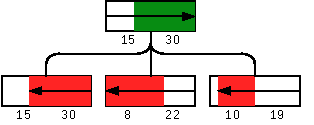
\includegraphics{figures/berliner1979/colour/berliner-step1.pdf}
    \fi
    \caption{The start of the B* search}
    \label{subfig:berliner_tree_init}
    \end{subfigure}
    \begin{subfigure}[t]{0.5\textwidth}
    \centering
    \ifMonochrome
        
\includegraphics{figures/berliner1979/monochrome/berliner-PB-step2.pdf}
    \else
        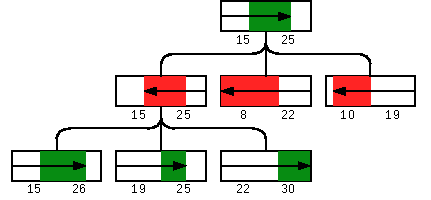
\includegraphics{figures/berliner1979/colour/berliner-PB-step2.pdf}
    \fi
    \caption{First node expanded with Prove-Best}
    \label{subfig:berliner_tree_PB1}
    \end{subfigure}
    
    \begin{subfigure}[t]{0.5\textwidth}
    \centering
    \ifMonochrome
        
\includegraphics{figures/berliner1979/monochrome/berliner-PB-step3.pdf}
    \else
        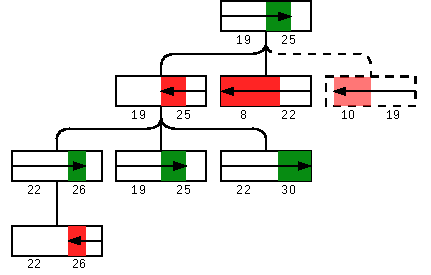
\includegraphics{figures/berliner1979/colour/berliner-PB-step3.pdf}
    \fi
    \caption{Second node expanded with Prove-Best}
    \label{subfig:berliner_tree_PB2}
    \end{subfigure}
    \begin{subfigure}[t]{0.5\textwidth}
    \centering
    \ifMonochrome
        
\includegraphics{figures/berliner1979/monochrome/berliner-PB-step4.pdf}
    \else
        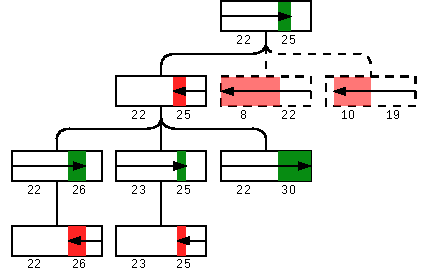
\includegraphics{figures/berliner1979/colour/berliner-PB-step4.pdf}
    \fi
    \caption{Separation has been achieved with Prove-Best}
    \label{subfig:berliner_tree_PB3}
    \end{subfigure}
    \caption{An example tree, based on an example by \protect\citeA{Berliner1979}, showing the application of the Prove-Best strategy for B*. Each rectangle represents a node, with its lower bound (left) and upper bound (right) depicted underneath. Nodes with arrows pointing right are maximising, and nodes with arrows pointing left are minimising. Dotted lines denote nodes that have become irrelevant to the search.}
    \label{fig:berliner_tree_PB}
\end{figure}

\begin{figure}
    \begin{subfigure}[t]{0.5\linewidth}
    \centering
    \ifMonochrome
        
\includegraphics{figures/berliner1979/monochrome/berliner-DR-step2.pdf}
    \else
        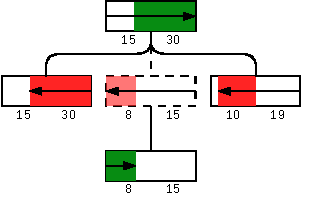
\includegraphics{figures/berliner1979/colour/berliner-DR-step2.pdf}
    \fi
    \caption{First node expanded with Disprove-Rest}
    \label{subfig:berliner_tree_DR1}
    \end{subfigure}
    \begin{subfigure}[t]{0.5\linewidth}
    \centering
    \ifMonochrome
        
\includegraphics{figures/berliner1979/monochrome/berliner-DR-step2.pdf}
    \else
        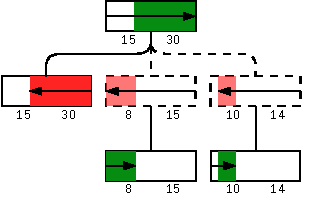
\includegraphics{figures/berliner1979/colour/berliner-DR-step3.pdf}
    \fi
    \caption{Separation has been achieved with Disprove-Rest}
    \label{subfig:berliner_tree_DR2}
    \end{subfigure}
    \caption{The same example tree, based on an example by \protect\citeA{Berliner1979}, from Figure \ref{fig:berliner_tree_PB} is depicted being explored with the Disprove-Rest strategy for B*. This example shows how the Disprove-Rest strategy can result in faster proofs than the Prove-Best strategy common for best-first search.}
    \label{fig:berliner_tree_DR}
\end{figure}

\subsubsection{Node Selection}
Finally, we describe how B* selects the next node to be expanded. As described above, B* selects either the node with the greatest upper bound or the node with the second greatest upper bound at the root node, depending on the decided strategy. However, the strategy may not always be selected. If the node with the greatest upper bound at the root does not also have the greatest lower bound, then Disprove-Rest can not lead to separation. Therefore, while the node with the greatest upper bound is not also the node with the greatest lower bound, B* uses the Prove-Best strategy. In addition, in best-first fashion, B* selects the best node at every depth other than the root for both Prove-Best and Disprove-Rest. This means to select the node with the greatest upper bound at maximising nodes and the node with the lowest lower bound at minimising nodes.

\subsection{Strategy Selection}
\label{subsec:strategySelection}
B*, as described above, requires a choice of strategy whenever the search backs up to the root. \citeA{Berliner1979} describes a heuristic approach to strategy selection, whereas \citeA{Sheppard2003} found a simpler approach to be effective in their implementation of B* for MAVEN in end-game play of Scrabble. This subsection describes some examples of strategy selection styles, although many others can exist and be applied to B*.

\subsubsection{Naive Approaches}
\label{subsec:strategySelection:Naive}
Naive approaches to strategy selection do not consider the structure of the tree or game-specific knowledge. The simplest example is to always select one strategy or the other. This results in \textbf{Always-PB} and \textbf{Prefer-DR} \cite{Anema2025}. Always-PB only ever selects Prove-Best. This is also referred to as `Best-First' by \citeA{Berliner1979}. Prefer-DR may select Prove-Best as well as Disprove-Rest, but always selects Disprove-Rest if it is applicable. As described before, B* may not select Disprove-Rest whenever the most optimistic node at the root is not also the least pessimistic node at the root, in which case Prove-Best is selected.

However, these variants do not take advantage of the benefits of the two strategies for B*. Naive approaches that may choose either strategy when both are applicable perform a lot better \cite{Anema2025} while still being simple. One such method is the method employed by \citeA{Sheppard2003} for the MAVEN program in end-game play of Scrabble: \textbf{Alternated}. This simply alternates the chosen strategy between Prove-Best and Disprove-Rest whenever both are applicable. Following with \citeA{Anema2025}, we implement this such that the alternation of strategies is halted when Disprove-Rest is not applicable and so that the first strategy selected is Prove-Best. Similarly, Anema also describes the \textbf{Randomised} approach, which randomly selects from either strategy when both are applicable. We can additionally define a parameter $p$ which determines how often Prove-Best will be selected, which we take to be $50\%$ unless stated otherwise.

\subsubsection{Heuristic Approaches}
\label{subsec:strategySelection:Heuristic}
Unlike the naive approaches described above, heuristic approaches usually incorporate information from the current state of the search tree to determine the next strategy. The approaches included in this thesis are two approaches described by \citeA{Berliner1979} in the original B* paper, but many others may be applied. The descriptions of these methods were modified to resolve ambiguities encountered during implementation. The $x$\textbf{D-criterium} selects Prove-Best or Disprove-Best based on the depth from which the upper bound of a node $i$ has been obtained ($d_i$). If the sum $\sum_{i=2}^x {d_i}^2$ is greater than or equal to ${d_1}^2$, then Prove-Best is selected, otherwise Disprove-Rest is selected. The children of the root node are sorted and numbered $1,2,\dots,x$ by decreasing upper bound, and any children with an upper bound below the greatest lower bound are excluded from the sum. The $x$\textbf{R-criterium} is the same as the $x$D-Criterium, but the values ${d_i}^2$, including $i=1$, are divided by the range of $i$, defined as $Range(i)=Upper(i)-Lower(i)$.
%
% \section{B* Variants}
% \label{sec:BstarVariants}
% \subsection{Searching with Probabilities: PB*}
% \begin{itemize}
%     \item Explain in more detail
%     \item pros: more effective, fewer nodes expanded
%     \item cons: needs much more memory per node for storing probability distributions
% \end{itemize}
% \subsection{Disprove-Best for B*}
% \begin{itemize}
%     \item Stress the problem DB-B* solves:
%         \begin{itemize}
%             \item the sub-problem of `false' best-nodes
%             \item designed for adversarial trees
%         \end{itemize}
%     \item DB-B* does not use extra memory space for distribution storage like PB*
%     \item could be combined with PB* for better performance at the cost of memory
%     \item (for more details, see Anema 2025)
% \end{itemize}

\begingroup
\linespread{0.98}\selectfont
\begin{adjustwidth}{0pt}{0pt}
\section{Proof-Number Search}
\label{sec:PNS}
This section describes the best-first adversarial search proofing technique Proof-Number Search (PNS) \cite{Allis1994} and two of its variants: $\text{PN}^2$ \cite{Breuker1998} and df-PN \cite{Nagai2002}. The section is structured as follows. First, Subsection \ref{subsec:PNS} describes PNS. Second, Subsection \ref{subsec:PN2} describes ${\text{PN}}^2$. Finally, Subsection \ref{subsec:dfPN} describes df-PN.

\subsection{Original Description}
\label{subsec:PNS}
As described in the introduction, PNS \cite{Allis1994} is a best-first algorithm for proving binary statements about nodes in an adversarial game tree.

\paragraph{Proof Numbers and Disproof Numbers.} PNS represents the binary quality of a node with proof and disproof numbers. Proof and disproof numbers represent the minimum search effort required to prove or disprove each node, respectively. We often write these in brackets like so: $\left(\text{pn}, \text{dn}\right)$, where the left `pn' is the proof number, and the right `dn' is the disproof number.
Therefore, each non-terminal node is initialised with proof and disproof numbers $\left(1,1\right)$, as at least one expansion is needed to either prove or disprove any leaf node. 
When a node is proven, we represent this with a proof number of 0 paired with a disproof number of $\infty$ like so: $\left(0,\infty\right)$. Likewise, disproven nodes are represented by $\left(\infty, 0\right)$. PNS by default keeps searching until the root node is either proven $\left(0,\infty\right)$ or disproven $\left(\infty,0\right)$.

\paragraph{AND/OR Trees.} For PNS specifically, it is useful to see the adversarial game tree as an AND/OR tree. This can be seen as OR nodes for the current player, and AND nodes for the opponent.
The first node is assumed, without loss of generality, to be an OR node, and alternating depths consist of either AND or OR nodes. For any node $n$, if $n$ is an OR node, then proving any child of $n$ proves $n$. However, $n$ is only disproven when all of its children are disproven. If $n$ is an AND node, then disproving any child of $n$ disproves $n$, but $n$ is only proven when all of its children are proven. This distinction between AND and OR nodes determines how (dis)proof numbers are updated at each node, as well as how the next node is selected at each node.

\paragraph{Most-Proving Node (MPN).}
PNS depends on the core idea of the Most-Proving Node (MPN). The MPN is a leaf node of the tree, which, if proven or disproven, contributes directly to the progress of the search at the root.
% Another way to look at it is that, if the selected MPN is expanded and (dis)proven, then the path of nodes leading to the MPN gets all their (dis)proof numbers decreased by 1.
The MPN is determined by choosing the node with the minimum proof number at OR nodes, and choosing the node with the minimum disproof number at AND nodes, until a leaf node is chosen.

\paragraph{Updating Values.}
In PNS, when a node $n$ is expanded, or one of its children is altered, then the (dis)proof numbers of $n$ will be determined as follows. If $n$ is an OR node, then the proof number of $n$ is the minimum proof number among the children of $n$, and the disproof number of $n$ is the sum of the disproof numbers of all children of $n$. If $n$ is an AND node, then its disproof number is the minimum disproof number among its children, and the proof number is the sum of proof numbers of all its children.

\paragraph{PNS Algorithm.}
The PNS algorithm \cite{Allis1994}, unmodified, is quite simple as a whole. As mentioned before, PNS keeps searching until the root node is either proven or disproven, iterating the following steps until that is the case:
\begin{enumerate}
    \item \textbf{Select} the most-proving node (MPN).
    \item \textbf{Expand} the MPN by adding all of its direct successors to the tree as new nodes.
    \item \textbf{Evaluate} each of the newly added nodes as either \textit{proven} $\left(0,\infty\right)$, \textit{disproven} $\left(\infty,0\right)$, or \textit{unknown} $\left(1,1\right)$.
    \item \textbf{Backpropagate} along the path to the root, updating all proof and disproof numbers along the way, until they no longer change.
\end{enumerate}
This basic implementation of PNS only depends on the structure of the tree and does not require any game-specific knowledge besides what is needed to generate and evaluate nodes as either proven, disproven, or unknown.

\subsection{\texorpdfstring{$\text{PN}^2$}{PN²}: Search on Larger Trees}
\label{subsec:PN2}
${\text{PN}}^2$, as described by \citeA{Breuker1998}, is a multi-level PNS variant with reduced memory usage. ${\text{PN}}^2$ effectively replaces the `\textbf{evaluate}' step of PNS, as described above, with another PNS search. This has the effect of increasing the information gained from each expansion of the first-level PNS, which reduces the overall size of its tree. However, to achieve this, the majority of the search effort is discarded at the end of every second-level PNS search, which negatively affects the computational cost of the search.
To control this effect, a size limit is applied to the second-level search, which is terminated early when the second-level tree exceeds its size limit. The second-level tree-size limit thus determines the trade-off between memory usage and computational efficiency.

\citeA{Breuker1998} describes two main approaches for setting this tree-size limit. The first of which is to set the limit of the second-level search to be the size of the first-level tree. We will refer to this approach as \textbf{max}. The second approach is to take a fraction between 0 and 1 of the previous limit. \citeA{Breuker1998} proposes the use of a logistic growth function to determine this fraction.
Let $x$ be the size of the first-level tree, then $f(x)$ is the fraction of $x$ to use as the second-level tree-size limit, as follows:
\begin{gather}
    f(x) = \frac{1}{1+e^{\frac{a-x}{b}}}
\end{gather}
where, $a$ and $b$ are the logistic growth parameters. We will refer to this approach as \textbf{logistic}. With this, the actual tree-size limit of the second-level PNS search is the minimum of $x\cdot f(x)$, or $x$ for \textbf{max}, and the remaining available memory $N-x$, where $N$ is the total available memory.

\subsection{df-PN: Search on any Size Tree}
\label{subsec:dfPN}
In the development of PNS techniques, a technique that helped reduce, or even trivialise, the memory usage of PNS beyond $\text{PN}^2$ \cite{Breuker1998} is df-PN \cite{Nagai2002}. Unlike ${\text{PN}^2}$, df-PN does not rely on storing the search tree itself in memory. It instead uses only the execution stack and a transposition table (TT) to store progress of the search, similar to depth-first search techniques. Despite the name, df-PN behaves mostly like a best-first algorithm. It selects nodes in much the same way PNS does, but does not back-up values to the root as frequently as PNS. This is thanks to the use of value thresholds on the (dis)proof numbers, which control when the search gets backed up. The overall algorithm is structured as a multiple iterative deepening search, which repeatedly calls itself on child nodes until a (dis)proof number threshold is met. The thresholds of a node are chosen at each step based on the (dis)proof numbers of its alternatives.
\end{adjustwidth}
\endgroup

\chapter{Saving Memory for B*}
\label{cht:SavingMemoryBstar}
The B* \cite{Berliner1979} technique, as described in the previous chapter, has been extended to PB* \cite{Palay1983} and Disprove-Best B* \cite{Anema2025} to increase its efficiency as measured by the number of nodes expanded to solve optimality for an adversarial game-tree. Whereas Palay and \citeA{Berliner1996} saw the most promise in a probabilistic approach for further development of B*, Anema notes promise in extending B* to a form with reduced memory usage. This chapter explores this by describing ways to reduce memory usage in B* and by describing two B* variants with reduced memory usage.

This chapter is structured as follows.
First, Section \ref{sec:BstarAdjustments} describes some adjustments we made to B* to reduce its memory usage and improve its performance on the test domain.
% First, Section \ref{sec:BstarAdjustments} describes how memory is managed in B*. Section \ref{sec:BstarAdjustments:Modifications} also describes some modifications we applied to B* in this thesis.
Second, Section \ref{sec:BstarSquared} introduces ${\text{B*}}^2$, a multi-level B* technique inspired by $\text{PN}^2$ \cite{Breuker1998}, which reduces the memory usage of B* at the cost of additional computation. Finally, Section \ref{sec:dfBstar} introduces df-B*, a multiple iterative deepening technique inspired by df-PN \cite{Nagai2002}, to reduce the memory usage of B* even further with a transposition table and value thresholds.

\section{Additional B* Adjustments}
\label{sec:BstarAdjustments}
This section describes additional adjustments to B* to improve the memory usage and general performance on the test domain of artificial game trees. However, these adjustments are not domain-specific and may be applied to any domain.
% This section describes how we manage the memory usage of B* without changing the algorithm significantly. It also describes two modifications we applied to B* to increase its performance on the test domain.

\paragraph{Memory Management.}
\label{sec:BstarAdjustments:Memory}
The main adaptation to reduce the memory usage of B* is also described by \citeA{Berliner1979}: \textbf{pruning irrelevant sub-trees}. Any child node, anywhere in the tree, with an upper bound below its parent's lower bound or a lower bound above its parent's upper bound can not affect the outcome of the search. Specifically, if a node's bounds do not overlap with its parent, and its removal does not lead to a change in the bounds of its parent, we prune the node and its subtree from memory entirely. The pruning of nodes generally occurs at the value update of nodes during back-propagation.

\begin{figure}[htbp]
    \centering
    \ifMonochrome
        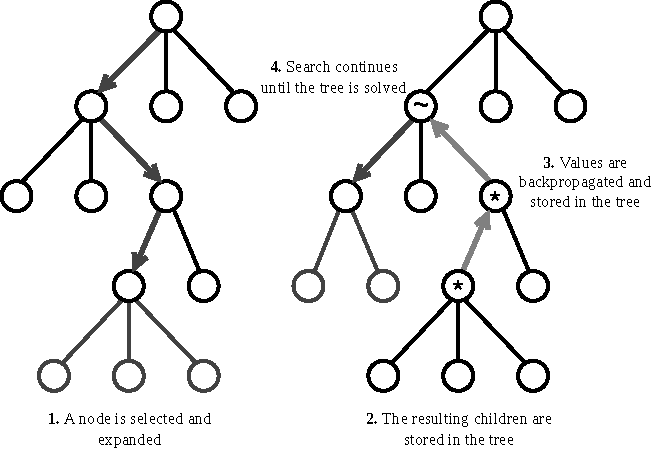
\includegraphics{figures/MemoryVisualizedBstarMono.pdf}
    \else
        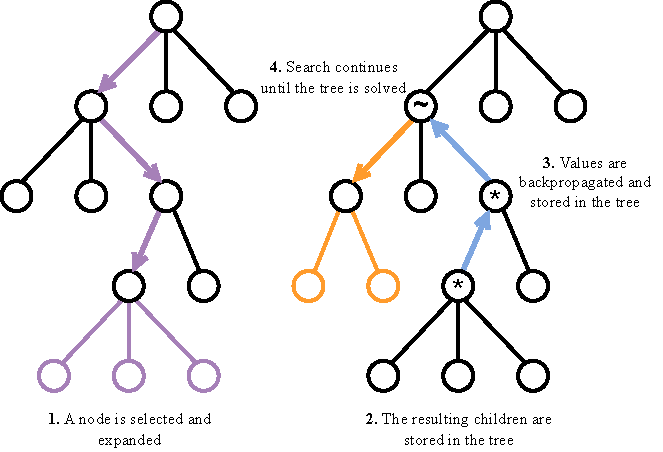
\includegraphics{figures/MemoryVisualizedBstar.pdf}
    \fi
    \caption{This diagram depicts how memory is handled in B* search. The entire tree is stored in memory, and expansions and evaluations are performed as described by \protect\citeA{Berliner1979}. Nodes are only removed from the tree if they have become irrelevant to the search through separation or through the separation of an ancestor.}
    \label{fig:memory_fig_bstar}
\end{figure}

\FloatBarrier
\paragraph{Novel Modifications.}
\label{sec:BstarAdjustments:Modifications}
We additionally describe two modifications to B* that preliminary experiments showed make B* perform better and make B* more comparable to ${\text{B*}}^2$ (see Section \ref{sec:BstarSquared}) on our choice of test domain as described in Chapter \ref{cht:ArtificialGameTrees}.

We introduce a \textbf{maximum to the number of consecutive back-propagations} without returning to the root node. A counter is incremented by 1 each time the search back-propagates and continues the search from an internal node. If this node is the root node, then the counter is reset to 0. The search is forcibly backed up to the root whenever this counter exceeds the maximum number of rootless updates $M$. In this thesis, we always use $M=1000$. This modification is included due to the infinite nature of the domain (Chapter \ref{cht:ArtificialGameTrees}) used in this thesis.

We also introduce a \textbf{modified selection protocol} at internal nodes (see Algorithm \ref{alg:BstarSelectAltInternal}). At any node, not including the root node, the selection of the next node defaults to the most optimistic child node $N_{opt}$. However, if $N_{opt}$ is not equal to the least pessimistic node $N_{pes}$, then we may select $N_{pes}$ instead.
We may only select $N_{pes}$ as the next node if its range is greater than 0, such that $N_{pes}$ is not a terminal node and has not yet been solved.
If these conditions are met, we select $N_{pes}$ with a probability of $P_{alt}$.
% meaning that we have not yet solved $N_{pes}$ and it is not a terminal node.
% If this is the case, we select $N_{pes}$ with a probability of $P_{alt}$.
% The pseudocode in Algorithm \ref{alg:BstarSelectAltInternal} describes how $N_{pes}$ is selected, with a random selection chance parameter $P_{alt}$. %, depending on the parameter $P_{alt}$.
% We may only select $N_{pes}$ as the next node if it is not a terminal node. If this is the case, we select $N_{pes}$ with a probability of $P_{alt}$ and $N_{opt}$ with a probability of $1 - P_{alt}$.
Preliminary experiments showed that a choice of $P_{alt}=0.3$ gives the best performance on our domain. In this thesis, we therefore always use $P_{alt}=0.3$. We decided to include this modification to adjust for a measure of uncharacteristically low performance of B* on large artificial game trees compared to ${\text{B*}}^2$ in preliminary experiments.

\begin{algorithm}[h!b]
\begin{algorithmic}[1]
\If{leastPes \textbf{is not} mostOpt \textbf{and} leastPes.range $>$ 0 \textbf{and} randomly$\left(P_{alt}\right)$}
\State nextNode $\coloneqq$ leastPes
\Else
\State nextNode $\coloneqq$ mostOpt
\EndIf
\end{algorithmic}
\caption{selectAlternative$\left(\text{leastPes, mostOpt}, P_{alt}\right) \to$ nextNode}
\label{alg:BstarSelectAltInternal}
\end{algorithm}

\FloatBarrier
\newpage
\section{A Multi-Level Approach to B*}
\label{sec:BstarSquared}
Several approaches have been applied to reduce the memory usage of the best-first adversarial solver technique PNS by \citeA{Allis1994}. These approaches can serve as inspiration for B* \cite{Berliner1979}, as it is also a best-first adversarial solver. One such approach is $\text{PN}^2$: a two-level PNS engine with the promise of ``PN Search with small memory’’ \cite{Breuker1998}. This section describes a B* variant inspired by $\text{PN}^2$ to allow B* to search larger trees with the same memory: The ${\text{B*}}^2$ algorithm.

This section is structured as follows. First, Subsection \ref{subsec:BstarSquaredAlgorithm} describes the ${\text{B*}}^2$ algorithm conceptually, stating its components and caveats. Second, Subsection \ref{subsec:Level2SizeLimit} discusses the implementation detail of second-level tree-size limits and lists some example functions to determine the size of the second-level tree based on the first-level tree. Finally, Subsection \ref{subsec:MultiLevelSearch} describes an extended variant of ${\text{B*}}^2$ that supports more than two levels of the search tree, generally: ${\text{B*}}^k$.
% Last, Subsection \ref{subsec:BstarSquaredPseudocode} provides pseudocode for ${\text{B*}}^2$ and ${\text{B*}}^k$.

\subsection{\texorpdfstring{${\text{B*}}^2$}{B*²} Search}
\label{subsec:BstarSquaredAlgorithm}
The main concept of ${\text{B*}}^2$ is the same as that of $\text{PN}^2$ \cite{Breuker1998}: a two-level search provides more information per node evaluation, leading to earlier termination and a smaller tree to store in memory. ${\text{B*}}^2$ is a search consisting of two levels of B* search. The first level builds the tree in the same manner as B* \cite{Berliner1979}, as it is described in Section \ref{sec:Bstar}, but does not use the usual evaluation function for the evaluation of the next node. Instead, a second-level search is initiated with the node to evaluate as its root. This second-level search may have a different strategy selection procedure and different stop conditions as the first-level search. When the second-level search terminates, the values backed up to its root are used to update the first-level search, and the rest of the second-level tree is discarded. This second-level search thus functions as a more `informative’ evaluation function for the first-level B* search tree, trading additional computation for lower memory usage.

\paragraph{Immediate Evaluation.}
${\text{B*}}^2$ is inspired by $\text{PN}^2$ \cite{Breuker1998}, but it differs in some aspects due to the inherent differences between PNS and B*. An important difference is as follows. $\text{PN}^2$ employs delayed evaluation for the first-level search and immediate evaluation for the second-level search. The concept of delayed evaluation is mentioned by \citeA{Allis1994} for PNS and refers to waiting to evaluate a node until it has been selected. Immediate evaluation instead refers to evaluating a node immediately after it has been added to the tree through expansion of its parent node. Delayed evaluation is relevant for reducing computation when the evaluation function is heavy to compute, such as for $\text{PN}^2$. However, we recommend the use of immediate evaluation for both the first- and second-level search of ${\text{B*}}^2$. Delayed evaluation for B* has limited utility and has not yet been formalised. If a maximising node has one or more of its children not yet evaluated, its lower bound will be a correct lower bound for the game-theoretical value, but its upper bound may not be, as it may widen when the last children are evaluated. This complicates the implementation of delayed evaluation in B*, as node selection and pruning depend on the correctness of bounds at all stages of the algorithm. Delayed evaluation for B* is not completely ruled out as a possibility, but has not been implemented in this research for this reason. Therefore, we apply only immediate evaluation for all levels of the search.

\paragraph{Stop Conditions.}
\label{subsec:BstarSquaredAlgorithm:StopConditions}
The second-level search for ${\text{B*}^2}$ may have different stop conditions than the first-level search, which are checked when the search backs up to its root. As usual with B*, the first-level search stops when separation is reached for the best child node of the root. Additionally, the search may terminate when physical limits on some resource or a time limit are reached, such as when the process runs out of memory. The second-level search may terminate earlier as its goal is not to prove the optimality of some move at its root, but to provide more information for the first-level search. We describe four stop conditions for the second-level ${\text{B*}}^2$ search: (1) separation, (2) size limit, (3) shallow irrelevance, and (4) deep irrelevance.

The first stop condition, \textbf{separation}, is the main stop condition for B* search, which is to halt the search when the proof for the best move at the root is complete.
For the second-level search, this amounts to stopping the search when only one of its children is relevant to the search. This stop condition is beneficial to ${\text{B*}}^2$ for two reasons: (a) separation reduces the set of children of a node, leading to fewer nodes being stored in the first-level tree when this node is expanded later, and (b) if continued after separation, the second-level search can no longer choose between Prove-Best and Disprove-Rest, which reduces the effectiveness of B* at that level.

The second stop condition is the \textbf{spatial limit} imposed on the search. This is triggered when the total number of nodes stored in the second-level tree exceeds a specified limit. How this limit is determined is described in Subsection \ref{subsec:Level2SizeLimit}, which regulates the degree to which it is enforced. To extend the search before reaching these spatial limits we implement the pruning of irrelevant sub-trees at the second-level search tree, just as we do for the first-level search.

The third stop condition is that of \textbf{shallow irrelevance}. A node is irrelevant when its bounds are always equal to or worse than at least one of its sibling nodes. If the second-level root is irrelevant with respect to the first-level tree, we say that the current sub-tree has become irrelevant. Shallow irrelevance stops the second-level search as soon as the direct irrelevance of the second-level root is detected. 
% We stop the search as soon as this is detected, because there is little overhead to verify, and it is worthwhile to do so, as any search done in irrelevant sub-trees does not advance the proof further.

The fourth and final stop condition is \textbf{deep irrelevance}. This is similar to shallow irrelevance, but in addition to checking the irrelevance of the current sub-tree at the parent of the second-level root, we check it along the entire line of ancestors leading up to the first-level root. This check continues until no node values are updated, just like a normal backup in B* search \cite{Berliner1979}. Additionally, if the backup leads back to the first-level root, we stop the second-level search if separation of any kind has been reached at the first-level root, as this completes the first-level search as well. Deep irrelevance checking adds a decent amount of extra overhead, as it requires a complete backup of values to the first-level root every time the second-level search reaches its root. This is why we present it separately from shallow irrelevance.
% TODO: implement this in code as described here!!!
%  *: stop conditions only tested in context of ‘B*²-Variant’ with ‘store-children-of-L2-search’**
% **: might not be properly implemented, needs to be tested
%           why expand() without using existing bounds?
%           ... I recall that it did not work well,
%           but it is best to document this with the experiments
% 

\paragraph{Strategy Selection.}
Strategy selection is performed whenever B* backs up changed bounds to the root. For ${\text{B*}}^2$, strategy selection may differ from the first-level search to the second-level search. The first-level search may use more computational effort to determine its strategy, as it can be offset by reducing the number of second-level searches that need to be made. Whereas the second-level search will perform strategy selection many more times during the search, and it is thus preferably fast. Therefore, it is advised to use heuristic approaches for strategy selection of the first-level search and to use a fast strategy selection for the second-level search. This can be, for example, a depth-based heuristic as described by \citeA{Berliner1979} for the first-level search and a naive strategy selection (see Subsection \ref{subsec:strategySelection:Naive}) for the second-level search.

%% TODO : put somewhere else
%% * For Berliner’s heuristics, we included the depth of level-2 search in the `depth of bounds'-value used to determine its strategy selection criterion
%% (maybe in experiments? artificial trees?)

\paragraph{Preservation of Bounds.}
\label{subsec:BstarSquaredAlgorithm:BoundsPreservation}
Finally, we discuss additional nuance on how ${\text{B*}}^2$ may keep or discard part of the second-level search tree after it concludes, as determined by the stop conditions described above. Because ${\text{PN}^2}$ uses delayed evaluation, \citeA{Breuker1998} decided to keep the children of the second-level root in memory after the second-level search terminates, unless the root was solved. However, Breuker does not mention whether the computed (dis)proof numbers of these children were also preserved, or how they were incorporated into the following first- and second-level searches. We therefore describe four separate approaches to bounds preservation in multi-level search, for the context of ${\text{B*}}^2$:
\begin{enumerate}
    \item \textbf{Full disposal} is the absence of bounds preservation. We keep the updated values of the second-level root and store them directly in the first-level tree. The rest of the second-level tree is discarded and will need to be re-created upon further examination of this node. This is the approach that ${\text{PN}}^2$ usually does not use, but that we have implemented for ${\text{B*}}^2$ as it is clear, consistent, easy to implement, and works well.
    \item \textbf{Re-search} is the approach most likely used by \citeA{Breuker1998}, where the children of the second-level root are not discarded after the second-level search terminates, unless this root is solved. As a result, the next possible nodes do not need to be recomputed if the second-level root node is expanded again later.
    The saved children may also retain their bounds as they were computed in the second-level search. These bounds can provide additional information to move ordering, node selection, and second-level stop conditions, such as shallow irrelevance, as described above. However, these children are not kept in the first-level tree as computed nodes and will be re-expanded upon further evaluation.
    \item \textbf{Windowed} is an additional consideration for the re-search approach. Aside from providing information to move ordering, node selection, and stop conditions, the saved bounds can also function as a search window. For B*, this works by pruning encountered nodes immediately if they appear irrelevant to the search when compared to the search window, while they may still appear to be locally relevant.
    \item \textbf{Keep bounds} is the approach where the children of the second-level root are not discarded, and are instead directly stored in the first-level tree. Children for which initial bounds are already present are then not evaluated further with a second-level search. This way, second-level searches are only initiated on alternating depths. These saved bounds are less informative than the root bounds resulting from the second-level search, but do not require an additional search as with the other methods.
\end{enumerate}
One key difference between ${\text{B*}}^2$ and ${\text{PN}}^2$ is that ${\text{B*}}^2$ does not perform delayed evaluation. As a result, children kept after the second-level search terminates are not necessarily used immediately afterwards. On the contrary, B* expands a node $n$, which initialises a second-level search on each child $c$ of $n$, then re-evaluates the bounds of $n$. A likely result is that the bounds of $n$ are altered, which results in a back-propagation of the search. Therefore, without delayed evaluation, we recommend the \textbf{full disposal} approach to bounds preservation for ${\text{B*}}^2$.
% Finally, because $\text{PN}^2$ uses delayed evaluation, Breuker included the feature that $\text{PN}^2$ stores the children of the second-level root, if it was not solved, after that search concludes. However, Breuker does not go into depth on how this may be implemented. 
% \begin{itemize}
%     \item ${\text{PN}}^2$ saves values of second-level root children if node was still `unknown'
%     \item Implementation detail not mentioned by Breuker:
%     \begin{itemize}
%         \item How are these saved values incorporated into the following first- and second-level search?
%         \item Are nodes saved even if the search does not return directly to the same spot?
%     \end{itemize}
%     \item Possible interpretations for ${\text{B*}}^2$:
%     \begin{enumerate}
%     \item \textbf{full disposal}: dispose of the entire second-level tree, keep only the root values
%         \begin{enumerate}
%             \item \underline{caveat}: backtracking through the first-level tree during second-level search is not possible or limited, as updated parent bounds are incomplete while searching their children. This can be worked around by using the normal evaluation function value as initial bounds for any node to be expanded with a second-level search, before the bounds get updated after the second-level search terminates.
%             \item This is the approach that ${\text{PN}}^2$ usually does not use. This is the approach we initially implemented for ${\text{B*}}^2$ as it is clear, consistent, easy to implement, and works well. The other approaches have also been implemented for comparison in Chapter \ref{cht:Experiments}.
%         \end{enumerate}

%     \item \textbf{re-search}: keep second-level root children in memory after second-level search terminates
%         \begin{enumerate}
%             \item \textbf{ignore}: saved bounds guide the selection of the next node, but do not affect any of the following second-level searches of those saved children's sub-trees.
%             \item \textbf{windowed search}: pruning irrelevant nodes in second-level search based on the saved parent's bounds (a node is considered irrelevant to the search when its upper-bound is below the saved parent's lower-bound or its lower-bound is above the saved parent's upper-bound); This includes the optimisation from the `ignore' strategy, but requires more modifications to the B* algorithm.
%             \item \textbf{keep-bounds}: keep the saved bounds as final bounds for the first-level tree, initiating a second-level search only on alternating depths. These saved bounds are less informative than the root bounds resulting from the second-level search, but do not require an additional search as with the other methods. The effects of this may be game-dependent, as we usually have trees alternate players on alternating depths. The depths at which full second-level searches are performed may also determine the effectiveness, depending on the game.
%         \end{enumerate}
%     \end{enumerate}
%     \item Additional things of note:
%     \begin{itemize}
%         \item B* continues search at the same spot in the first-level tree if the expansion (second-level search) did not alter the parent's bounds from their previous value. Because ${\text{B*}}^2$ increases the information gained from expansions, the probability of bounds getting altered is increased, so the search likely does not continue from the same spot. This means that saved bounds may not actually end up being used, or may end up being used later on. Search may return to the same spot after a back-propagation, but this is not guaranteed.
%         \item ${\text{PN}}^2$ uses delayed evaluation, which (for reasons described in an earlier paragraph) ${\text{B*}}^2$ does not. Therefore, after second-level search terminates with `unknown', the same node needs to be expanded in ${\text{PN}}^2$, but this is not needed in ${\text{B*}}^2$ because we use immediate evaluation.
%     \end{itemize}
% \end{itemize}

%
%%%% Rewrite this in own words!: %%%%
%
% The way in which partial search results are retained between first- and second-level searches requires careful consideration. In ${\text{PN}}^2$, if a second-level search returns the value `unknown' for its root, the children of that root are preserved in memory while the rest of the second-level tree is discarded. Breuker's description does not detail how these saved child nodes are subsequently used when the search returns to that part of the tree. For ${\text{B*}}^2$, we must define this behaviour explicitly. Several interpretations are possible, each with different implications for the algorithm's memory use and search efficiency.
%
% The first option is to dispose of the entire second-level tree after each evaluation, keeping only the backed-up bounds for the root node in the first-level tree. This approach is simple and consistent. A potential difficulty is that backtracking through the first-level tree during a later second-level search could be affected, because the bounds of a parent node may be incomplete while its children are being searched. This can be addressed by initialising the bounds of any node slated for a second-level search with the value from the standard evaluation function, before updating them when the second-level search finishes. This full-disposal method is straightforward to implement and was our initial choice for ${\text{B*}}^2$.
%
% Alternatively, we can keep the children of the second-level root in memory after the search ends. This opens several sub-options. The simplest is to ignore these saved subtrees in subsequent second-level searches, using them only to guide node selection in the first-level tree. A more involved method is to use the saved parent bounds to prune irrelevant nodes in future second-level searches; a node is considered irrelevant if its value cannot affect the parent's bounds. This `windowed search' approach requires more modifications to the B* algorithm. A third variant is to treat the saved bounds as final for the first-level tree, performing a full second-level search only on alternating depths. The effectiveness of this `keep-bounds' method may depend heavily on the game, as tree depth often correlates with player turns.
%
% It is also worth noting that B* tends to continue searching from the same node in the first-level tree only if an expansion does not change the parent's bounds. Since ${\text{B*}}^2$ aims to gain more information per expansion, bounds are more likely to be updated, making it less probable that the search will remain at the same spot. Consequently, saved bounds may not be used immediately, or may be used only after some backtracking. Finally, because ${\text{B*}}^2$ uses immediate evaluation for all nodes—unlike ${\text{PN}}^2$, which uses delayed evaluation at the first level—there is no need to expand a node again after a second-level search returns an `unknown' value. The bounds are updated immediately, and the search moves on.

\subsection{Second-Level Tree-Size Limit}
\label{subsec:Level2SizeLimit}
Similar to ${\text{PN}}^2$ \cite{Nagai2002}, we apply a tree-size limit to the second-level search of ${\text{B*}}^2$. Subsection \ref{subsec:PN2} describes two approaches for determining tree-size limits in ${\text{PN}}^2$. These approaches are also applied to ${\text{B*}}^2$, as described here.

The \textbf{max} tree-size limit is the technique of setting the size limit of the second-level search equal to the current size of the first-level tree. This is a simple and effective way to set the second-level limit. 
However, \citeA{Breuker1998} notes how this approach made ${\text{PN}}^2$ take much longer to solve small problems. To address this, the \textbf{logistic} size limit was introduced. Here we take the limit of the second-level tree to be a fraction $f(x)$ of the size of the first-level tree $x$, which is defined as:\label{subsec:Level2SizeLimit:Sigmoid}
\begin{gather}
    f(x) = \frac{1}{1+e^{\frac{a-x}{b}}}
\end{gather}
where $a$ and $b$ are the logistic growth parameters, which control for the shape of the logistic growth curve. For our experiments, we applied values of $a=500\text{\thsep}000$ and $b=50\text{\thsep}000$.

\noindent Ultimately, for both approaches, we restrict the actual tree-size limit by the remaining available memory $N-x$, where $N$ is the total available memory. Such that the memory limit for \textbf{max} is:
\begin{gather}
    \text{MaxLimit} = \min\left[x,N-x\right]
\end{gather}
And the memory limit for \textbf{logistic} is:
\begin{gather}
    \text{LogisticLimit} = \min\left[\frac{x}{1+e^{\frac{a-x}{b}}}, N-x\right]
\end{gather}
% \textit{``if ${\textit{B*}}^\textit{2}$ is a trade of computation for memory saving, then the second-level tree-size limit is the pricing slider''}
% \begin{itemize}
    % \item As described by \cite{Breuker1998} (Breuker1998)
    % \item Limiting L2 tree size to L1 tree size makes sense and works well
    % \item Smaller tree-size limits may perform better, but limit the level of memory reduction
    % \item Should be evaluated on two fronts: \textbf{Memory reduction} \& \textbf{Node expansions}
% \end{itemize}
% \paragraph{Sigmoid-based limits.}

\begin{figure}[hbpt]
    \centering
    \ifMonochrome
        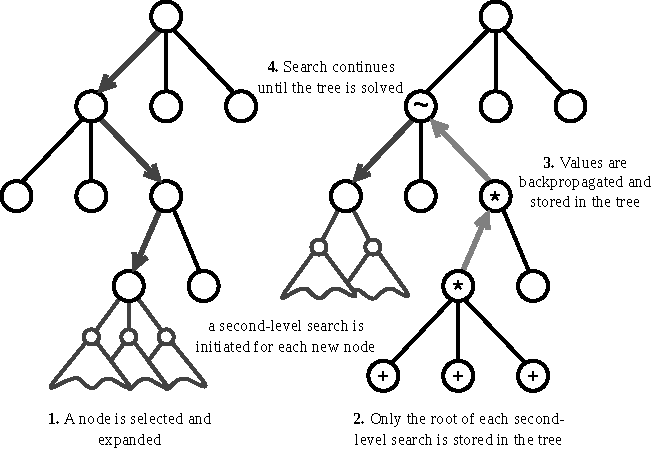
\includegraphics{figures/MemoryVisualizedBstarSquaredMono.pdf}
    \else
        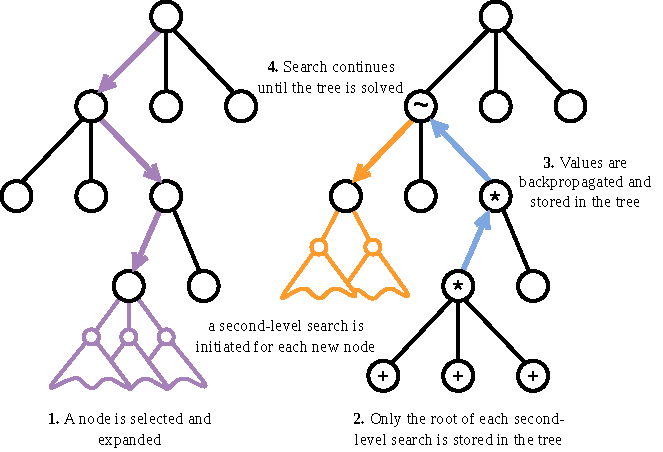
\includegraphics{figures/MemoryVisualizedBstarSquared.pdf}
    \fi
    \caption{This diagram depicts how memory is handled in ${\text{B*}}^2$ search. Only the first-level tree is stored in memory throughout the search. Evaluations are performed through a second-level B* search, the tree of which is discarded after its termination. The values of newly expanded nodes are more informative as a result, leading to a smaller tree overall.}
    \label{fig:memory_fig_bstarsquared}
\end{figure}

\subsection{Extension to Many-Levelled Search}
The ${\text{B*}}^2$ search technique described above allows B* to search larger trees, which would usually not fit in memory, by structuring the search in two levels. This subsection describes the generalisation from two-level ${\text{B*}}^2$ to $k$-level ${\text{B*}}^k$ search. This technique reduces memory usage further, at the cost of additional computation, for increasing values of $k$.

\subsubsection{Motivation}
\label{subsec:MultiLevelSearch}
The idea of utilising a second-level search as an evaluation function for the first-level search, which inspired ${\text{PN}}^2$ \cite{Breuker1998}, was taken from an earlier paper on Bayesian Search by \citeA{BaumSmith1997}. The paper mentions multi-level search as a possible extension to reduce memory usage to ``roughly a square root'', while ``imposing speed reductions of only a constant factor''. This is also what allows ${\text{B*}}^2$ to reduce its memory usage at the cost of additional computation. Effectively, the multi-level search enhances the evaluation function for B* search, which allows the search to terminate earlier. Similarly, we can use a B* search as the evaluation function of a ${\text{B*}}^2$ search to create a three-level ${\text{B*}}^3$ search.

When we apply the prediction of square-root memory usage by \citeA{BaumSmith1997} to B*, then a $k$-level search may expect roughly $\sqrt[k]{N}$ of nodes stored in memory compared to $N$ nodes for a plain B* search. Therefore, the motivation behind ${\text{B*}}^k$ is that, if a problem is too large to be solved with B* or ${\text{B*}}^2$ within the memory limitations, then some greater choice of $k$ may exist for which ${\text{B*}}^k$ can solve the problem.
However, in all cases, there has to be at least enough memory available to store the execution stack of the search, which is in the order of the maximum depth reached by the search.
% However, this is not a definitive law, as there may not be enough resources available to store the full line of successors leading up to the maximum depth reached by the program during the search.
Additionally, the square-root prediction, combined with the overhead of search, suggests diminishing returns for larger values of $k$. However, this does not matter as much if ${\text{B*}}^k$ allows problems to be solved that could not be solved before.

\subsubsection{Overhead}
When implementing and applying ${\text{B*}}^k$, note that the benefit of increasing the number of levels $k$ is primarily in the reduction of memory usage. Every additional level of nesting increases not only the number of nodes expanded by the search, but also the level of overhead for each step of the first-level search. Increasingly nested levels of search contribute more to computational overhead while contributing less, per tree, to the total search effort. Any overhead from search initialisation, stop conditions, strategy selection, and size limit calculations is magnified for the highest levels of the search. Therefore, it is good to minimise $k$ for the resources available, to increase the efficiency of the algorithm.

\subsubsection{Strategy Selection}
Different strategy selection procedures may be chosen for every level of the ${\text{B*}}^k$ search. More complex methods, like the depth-based criterion by \citeA{Berliner1979}, require additional overhead, which is magnified at higher levels of the search. At these levels, we find that it is a safe default to always select Prove-Best. Alternating between Prove-Best and Disprove-Rest, or randomly selecting the strategy, are also good choices for higher-level searches. The latter can be tuned by choosing the chance of selecting Prove-Best $p$ (see Subsection \ref{subsec:strategySelection}) for the best results. Similarly to ${\text{B*}}^2$, it may be worthwhile to expend extra effort for strategy selection in the first-level search, as each expansion of the first-level tree initiates a large amount of search effort by a ${\text{B*}}^{k-1}$ search on the children of the expanded node.

\subsubsection{Tree-Size Limits}
Tree-size limits get more complex with multiple levels of search, as there are many possible configurations. However, it may be ill-advised to maximise all limits. If all levels of the search use the \textbf{max} tree-size limit, then each $k$-level search creates and deletes as many nodes as are present in the first-level tree.
% $L_k = N_1$, so every search maximises its memory usage. 
This would maximise the amount of search that is discarded after a nested search terminates, whereas a smaller search might have saved on computation. However, stricter tree-size limits do increase memory usage, but this effect is less noticeable for highly nested searches. It is therefore advised to taper off the tree-size limits of higher-level searches, such that the second-level search has more allocated memory, whereas the third-, fourth-, and higher-level searches get decreasing amounts of memory. For example, we found that a configuration for ${\text{B*}}^3$ with a \textbf{logistic} size limit, as described in Subsection \ref{subsec:Level2SizeLimit:Sigmoid}, for the second-level tree and a small fixed size limit for the third-level tree showed promise.

\subsubsection{Stop Conditions}
${\text{B*}}^k$ may also have different stop conditions for each level of the search. The second-level stop conditions can be chosen the same way as for ${\text{B*}}^2$. Higher-level searches magnify the overhead of all operations, including the stop condition, which is checked whenever the search backs up to the root. Separation is generally a cheap condition to check, so it can usually be included at all levels of the search. Shallow and deep irrelevance, as described in Subsection \ref{subsec:BstarSquaredAlgorithm}, have some additional overhead, which may outweigh their benefits for higher-level searches. Additionally, if tree-size limits are set to taper off for higher-level searches, then stop conditions likely do not affect the higher levels of the search as much. It is more likely that the search is terminated by running out of resources when the tree-size limits are small. Reducing the complexity of stop conditions is therefore advised for higher levels of the search.

% \subsection{\texorpdfstring{${\text{B*}}^2$}{B*²} Pseudocode}
% \label{subsec:BstarSquaredPseudocode}
% \begin{algorithm}[h]
% \begin{algorithmic}[1]
% \State 
% % \State \textbf{Let} eval($n$) \textbf{be}
% % \State \hspace{3em} M = sizeOf($r$)
% % \State \hspace{3em} res = B*($n,H_2$).limitedBy(M)
% % \State \hspace{3em} \Return lowerbound(res), upperbound(res)
% % \State B*($n,H_1$).withEval(eval($n$))
% \end{algorithmic}
% \caption{${\text{B*}}^2\left(n,H_1,H_2\right)$}
% % % \vspace{1ex}
% % % This procedure does nothing.
% \label{alg:BstarSquared}
% \end{algorithm}
%%%%%%
% \begin{algorithm}[H]
% \begin{algorithmic}[1]
%     \State current $\coloneqq$ root
%     \State expand(current)
%     \State Update(current, $k-1$, $H_1,\dots,H_k$)
%     \While{\textbf{not} separation at root}
%         \State \textbf{if} current is root \textbf{then} SelectStrategy(root, $H_1$)
%         \State current $\coloneqq$ SelectNext(current, root)
%         \State expand(current)
%         \State current $\coloneqq$ Update(current, $k-1$, $H_1,\dots,H_k$)
%     \EndWhile\\
%     \Return best child node at root
% \label{__algstep_0}
% \end{algorithmic}
% \caption{${\text{B*}}^k$(root, $k$, $H_1, \dots,H_k$) $\to$ bestMove}
% \label{alg:1-BstarMain}
% \end{algorithm}

% \vspace{-2ex}

% \begin{algorithm}[H]
% \begin{algorithmic}[1]
% \setcounterref{ALG@line}{__algstep_0}
%     % \If{$ChildBestOpt(\text{root}) \neq ChildBestPes(\text{root})$}
%     \If{mostOpt(root) is not leastPes(root)}
%         \State strategy $\coloneqq$ ProveBest
%     \Else
%         \State strategy $\coloneqq$ $H$(root).decide\{ProveBest \textbf{or} DisproveRest\}
%     \EndIf
% \label{__algstep_1}
% \end{algorithmic}
% \caption{SelectStrategy(root, $H$)}
% \label{alg:2-SelectStrategy}
% \end{algorithm}

% \vspace{-2ex}

% \begin{algorithm}[H]
% \begin{algorithmic}[1]
% \setcounterref{ALG@line}{__algstep_1}
%     \If{current is root}
%         \If{strategy is DisproveRest}
%             \State\Return secondMostOpt(root)
%         \Else
%             ~~\Return mostOpt(root)
%         \EndIf
%     \Else
%         \State \Return selectAlternative(leastPes(root), mostOpt(root), $P_{alt}$)
%     \EndIf
% \label{__algstep_2}
% \end{algorithmic}
% \caption{SelectNext(current, root) $\to$ next}
% \label{alg:3-SelectNext}
% \end{algorithm}

% \vspace{-2ex}

% \begin{algorithm}[H]
% \begin{algorithmic}[1]
% \setcounterref{ALG@line}{__algstep_2}
%     \If{$j$ is 0 \textbf{or} node already has bounds}
%         \State boundsChanged $\coloneqq$ computeAndSetBounds(node)
%     \Else
%         \State node$'$ $\coloneqq$ copy(node)
%         \State $N \coloneqq$ size(tree of node.root
%         \State $L \coloneqq$ $\min\left[N, M-N\right]$
%         \State ${\text{B*}}^j$(node$'$, $L$, $j$, $H_2, \dots,H_k$)
%         \State node.setBounds(node$'$.bounds)
%     \EndIf
%     \If{boundsChanged \textbf{and} node is not root}
    
%     \Return Update(parent of node, $M$, $j$, $H_1,\dots,H_k$)
%     \Else~\Return node
%     \EndIf
% \end{algorithmic}
% \caption{Update(node, $M$, $j$, $H_1,\dots,H_k$) $\to$ next}
% \label{alg:4-Update}
% \end{algorithm}

\newpage

\section{A Depth-First Approach to B*}
\label{sec:dfBstar}
Another approach to reduce the memory usage of best-first search techniques is to restructure the search as a depth-first search. An example of this is the PNS variant df-PN \cite{Nagai2002}, which we describe in Subsection \ref{subsec:dfPN}. We apply this approach to B* as well, which results in the depth-first B* variant df-B*. This section describes this novel search technique and is structured as follows. First, Subsection \ref{subsec:dfBstar:description} describes the df-B* technique from its inspirations to its formal definition, and finally, its pseudocode. Second, Subsection \ref{subsec:dfBstarChallenges} presents some challenges and implementation details for df-B* that may need to be taken in consideration when applying this technique to other domains.

\subsection{df-B* Search}
\label{subsec:dfBstar:description}
For the depth-first approach to B*, a major difference is the lack of a search tree stored in memory, as B* and ${\text{B*}}^2$ do. Instead, depth-first search relies on a transposition table (TT) to store the results of sub-tree searches. The technique we introduce, df-B*, is heavily inspired by df-PN \cite{Nagai2002}, which we describe in Subsection \ref{subsec:dfPN}.
% Another approach to reducing memory is the depth-first approach, which does not store the tree in memory as ${\text{B*}}^2$ and ${\text{B*}}^k$ do, but instead relies on a transposition table (TT) for storage. This approach, called df-B*, is heavily inspired by df-PN \cite{Nagai2002}, which we describe in Subsection \ref{subsec:dfPN}.
As with df-PN, we use thresholds to control the effort expended by recursive and iterative calls of the search function. However, unlike df-PN's (dis)proof numbers, B*'s bounds and their subsequent thresholds do not provide true information on the difficulty or expanse of search needed to prove a certain goal. They may indicate it, but there are no guarantees beyond those that ensure B* terminates exactly when the optimal move is proven. This implementation may therefore come with some caveats resulting from that key difference. First we describe the adaptations needed to construct df-B*, as viewed from the perspecfive of df-PN.

\subsubsection{From df-PN to df-B*}
The main additions and modifications needed to turn df-PN into df-B* come from the differences between PNS and B*.

First, PNS uses the same search procedure at the root as anywhere else in the tree, but B* does not, and df-B* cannot either. For B*, node selection at the root differs from node selection at all other nodes.
% For df-B*, this also affects the choice of thresholds, as discussed later.
% As we will discuss a bit later in this section, the node selection and choice of thresholds at the root differ from those at all other nodes.
We therefore describe two main loops of the df-B* algorithm: root-level and low-level. The root-level loop, or simply root-level search, repeatedly decides the strategy and calls low-level searches until separation has been reached. The low-level search iteratively calls itself through Multiple Iterative Deepening (MID), controlled by node value thresholds, while utilising a TT for storage, similar to df-PN \cite{Nagai2002}.

Second, as mentioned earlier, (dis)proof numbers provide different information than B* minimax bounds do. \citeA{Nagai2002} describes df-PN with thresholds propagating based on (dis)proof numbers of competitors, either by summing them or by taking the value of a competitor $+1$. 
 % With this, the search down a specific branch continues as long as the MPN is an ancestor of the current node. B*'s bounds 
Bounds for B* are heuristic values and thus are not easily described as discrete units of effort. To address this, we take inspiration from the $1+\epsilon$ trick for df-PN by \citeA{PawlewiczLew2007}: thresholds grow by a constant factor multiplied by the (dis)proof numbers. Instead of setting the `target' of a search call to the necessary threshold $+1$, we let it grow by a multiplicative factor of $1+\epsilon$. This extends well to B*, as we can take the threshold $T$, which, when reached, would change the behaviour of B* but not terminate the search, and set our new threshold to $T \pm \epsilon\cdot\left(U-L\right)$.
This way of setting thresholds reduces frequent switching between two or more nodes with similar values, by taking longer to stop searching a branch that is no longer optimal.
% This way of setting thresholds makes df-B* commit to search a chosen branch further than would be considered the optimal path by B*, reducing inefficiencies from frequent switching between nodes with similar values.
% This way of setting thresholds reduces progress lost from frequent switching between two or more nodes with similar values by committing to search a chosen branch a bit further than would be considered the optimal path by B*.
To make df-B* behave as closely to B* as possible, we can set $\epsilon$ close to $0$. The exact value of $\epsilon$ may depend on the domain, but is always a factor of the bounds of a node. If two evaluation functions can be mapped linearly, then df-B*$\left(\epsilon\right)$ will behave the same way on both.

Third, PNS only knows one strategy and one type of behaviour, but B* has two strategies: Prove-Best and Disprove-Rest. Strategies for df-B* are handled in the root-level search and are determined heuristically. Heuristics that can be used for B* should also apply to df-B*, given that the necessary information does not require storing the search tree in memory. An adaptation specifically for df-B* is the addition of the parameter $\sigma$ , which performs the same role as $\epsilon$, but only for the root-level search. Increasing $\epsilon$ makes the search behave more aggressively and more efficiently in space-limited scenarios \cite{PawlewiczLew2007}, at the low-level search. But $\sigma$ determines how often the search will back up to the root, at the root-level search. In df-PN, there is no crucial difference between $\epsilon$ at the root and $\epsilon$ at internal nodes. But for df-B*, the amount of leniency in thresholds at the root controls the frequency of strategy reconsideration, the quality of which affects the efficiency of B* \cite{Berliner1979}. The parameters $\epsilon$ and $\sigma$ thus control the balance between memory efficiency and the frequency of B* strategy selection during the search.

\subsubsection{An Overview of df-B*}
We implement df-B* based on an unmodified B* search, where the only adaptations made are those required to structure B* as a depth-first search as inspired by df-PN.
The following sketch shows an overview of df-B* divided into the root-level and low-level search procedures:\vspace{2ex}
% df-B* is an algorithmic concept that applies the principles of df-PN to B*. However, this is not a thoroughly tested technique and may need revisions in later research. The following sketch shows an overview of df-B* divided into the root-level and low-level search procedures:\vspace{2ex}
\makebox[\linewidth]{
\fbox{
\begin{minipage}[c]{0.8\linewidth}
    \paragraph{Root-level df-B*}: $\sigma\in\left(0,\frac{1}{2}\right)$\\
    At root node $r$, sort children $N_1,N_2,\dots,N_b$ by decreasing upper bound;\\
    Define upper and lower bounds as $U_i$ and $L_i$ for any node $N_i$;\\
    \textbf{\textit{While $L_1 < U_2$ do:}}
    \begin{addmargin}[1em]{2em}
        \textbf{If} $L_1 < \max L_i$: Set $s=1$;\\
        \textbf{Else} heuristically decide $s=1$ (PB) or $s=2$ (DR);\\
        Start searching at $N_s$ until thresholds exceeded:\\
        \phantom{}\hspace{1em} $t_s = \min\left[U_2, L_s+\sigma\cdot\left(U_s-L_s\right)\right]$;\\
        \phantom{}\hspace{1em} $\tau_s=\max\left[L, U_s-\sigma\cdot\left(U_s-L_s\right)\right]$;\\
    \end{addmargin}
    \vspace{-3ex}
    \paragraph{Low-level df-B*}: $\epsilon\in\left(0,1\right)$\\
    Searching at node $n$ with bounds $L, U$ and thresholds $t, \tau$;\\
    \textbf{\textit{While} $L < t$ and $\tau < U$ and $L < U$ \textit{do:}}
    \begin{addmargin}[1em]{2em}
        \textbf{If} $n$ is Minimising:\\
        \phantom{}\hspace{1em} Sort children $N_1,N_2,\dots,N_b$ by increasing lower bound;\\
        \phantom{}\hspace{1em} Start searching at $N_1$ until thresholds exceeded:\\
        \phantom{}\hspace{2em} $t_1=\min\left[t, L_2+\epsilon\cdot\left(U_1-L_1\right)\right]$;\\
        \phantom{}\hspace{2em} $\tau_1=\tau$;\\
        \phantom{}\hspace{1em} Maintain $L=\min L_i$ and $U=\min U_i$;\\
        \textbf{If} $n$ is Maximising:\\
        \phantom{}\hspace{1em} Sort children $N_1,N_2,\dots,N_b$ by decreasing upper bound;\\
        \phantom{}\hspace{1em} Start searching at $N_1$ until thresholds exceeded:\\
        \phantom{}\hspace{2em} $t_1=t$;\\
        \phantom{}\hspace{2em} $\tau_1=\max\left[\tau, U_2-\epsilon\cdot\left(U_1-L_1\right)\right]$;\\
        \phantom{}\hspace{1em} Maintain $L=\max L_i$ and $U=\max U_i$;\\
    \end{addmargin}
\end{minipage}
}}\vspace{2ex}
Thresholds at the root- and low-level search are chosen to stop the search immediately when separation is reached at the root, so there is no extra computation regardless of $\epsilon$ or $\sigma$. We have also provided pseudocode for the root-level df-B* (see Algorithm \ref{alg:dfBstar}) and the low-level df-B* (see Algorithm \ref{alg:MIDdfBstar}). The pseudocode shows the usage of a transposition table (TT) for df-B*, as this technique is designed to work with a TT.
The main information stored in the TT for df-B* is the lower and upper bounds $L,U$ for each node $n$. Thresholds do not need be stored, as they are computed from the top down during the search. If a TT entry for $n$ already exists, then we keep the values that give the tightest bounds (by smallest range $R=U-L$). If a TT entry exists for a different node $m$ with the same key as $n$, then we require a replacement scheme \cite{Nagai2002}. For this thesis, we apply the `always replace' scheme, which means we always overwrite the entry of $m$ in favor of the newer entry $n$.
Other replacement schemes are discussed in Subsection \ref{subsec:dfBstarChallenges}, along with other information which may help with the implementation of df-B*.
% This may prioritise saving nodes that are more likely to be re-used, or saving nodes that require the most effort to be recomputed. A specific difficulty with depth-first traversal of the tree is that we cannot always determine whether $m$ is still relevant to the search or not, as it may be locally relevant but globally irrelevant at the same time. The simplest solution is to always replace old entries with the same key, but better approaches may be possible.
% ... should save the entry that requires the most amount of search effort to compute anew.
% A good measure of effort is the size of the frontier of each node's sub-tree: the number of relevant leaf-nodes in this sub-tree. This can be computed during the search. An alternative measure can be the depth of a node, as a lower depth node, closer to the root, may 
% Setting up a transposition table for df-B* is similar: store the lower and upper bounds $L,U$ for each node. Collisions can be resolved by the tightest bounds for the same node and by the largest frontier for different nodes. Tighter bounds (higher $L$, lower $U$) on the same node mean more work has been performed there, because bounds for B* are nonincreasing. A good measure of effort to compare different nodes with each other is the size of the frontier of each node's subtree. This quantity can be computed during the search. An alternative measure can be the depth of a node, as a lower depth node, closer to the root, may be visited more frequently.

\begin{algorithm}[p]
\begin{algorithmic}[1]
\State $N_i\coloneqq$ CreateChildren$\left(r\right)$
\State $L_i,U_i \coloneqq$ GetBounds$\left(N_i\right)$\Comment{From evaluation function}
\State SortChildren$\left(r\right)\to N_1,\dots,N_b$\Comment{By decreasingly optimistic}
\While{$\left(L \coloneqq\max_i L_i\right) < U_2$}\Comment{$r$ is assumed to be a MAX node}
    \State \textbf{if} $L_1 < L$ \textbf{or} $H.\text{UseProveBest}\left(r\right)$ \textbf{then} $s \coloneqq 1$
    \State \textbf{else} $s \coloneqq$ 2
    \State $t_s \coloneqq \min\left[U_2, L_s+\sigma\cdot\left(U_s-L_s\right)\right]$
    \State $\tau_s \coloneqq \max\left[L, U_s-\sigma\cdot\left(U_s-L_s\right)\right]$
    \State MID$\left(N_s, t_s, \tau_s, \epsilon\right) \to L_s,U_s$
    \State SortChildren$\left(r\right)\to N_1,\dots,N_b$
\EndWhile
\end{algorithmic}
\caption{df-B*$\left(r,\sigma,\epsilon,H\right)$}
% \vspace{1ex}
This procedure initiates the depth-first B* (df-B*) search at the root node $r$. df-B* searches an adversarial or non-adversarial tree with an evaluation function to provide lower and upper bounds on the game-theoretical value. The search terminates when the optimal next move at the root has been determined.
% This algorithm runs in $O(d\cdot b)$ space, where $d$ is the search depth and $b$ is the average branching factor of the tree.
% Details on the use of a transposition table are not provided here, as it was out of scope for this thesis. 
\label{alg:dfBstar}
\end{algorithm}

\begin{algorithm}[p]
\begin{algorithmic}[1]
\State $L,U \coloneqq$ GetBounds$\left(n\right)$\Comment{Passed on from previous call}
\If{$L\ge t$ \textbf{or} $U \le \tau$ \textbf{or} $L=U$} \label{lst:MIDstopConditionList1}
    \State SaveBounds$\left(n,L,U\right)$\Comment{Put in Transposition Table}
    \State \Return $\left(L, U\right)$
\EndIf
\State $N_i \coloneqq$ CreateChildren$\left(n\right)$
\State SaveBounds$\left(n,L,U\right)$ \Comment{Cycle avoidance \cite{Nagai2002}}
\While{true}
    \If{$L \ge t$ \textbf{or} $U \le \tau$ \textbf{or} $L=U$} \label{lst:MIDstopConditionList2}
        \State SaveBounds$\left(n,L,U\right)$
        \State \Return $\left(L, U\right)$
    \EndIf
    \State $L_i,U_i \coloneqq$ GetBounds$\left(N_i\right)$\Comment{Retrieve from TT or compute anew}
    \State SortChildren$\left(n\right)\to N_1,\dots,N_b$\Comment{By decreasingly optimistic}
    \State Discard$\left(N_i\text{ where }L_i > U \text{ or } U_i < L\right)$\Comment{Prune irrelevant nodes}
    \If{IsMinimising$\left(n\right)$}
        \State $t_1 \coloneqq \min\left[t,L_2+\epsilon\cdot\left(U_1-L_1\right)\right]$\Comment{If no $N_2$ present, $t_1=t$}
        \State MID$\left(N_1,t_1,\tau,\epsilon\right)\to L_1,U_1$
        \State $\min_i L_i, \min_i U_i \to L, U$\label{lst:MIDupdateBoundsMin}
    \Else{ \textbf{if} IsMaximising$\left(n\right)$ \textbf{then}}
        \State $\tau_1\coloneqq\max\left[\tau,U_2-\epsilon\cdot\left(U_1-L_1\right)\right]$\Comment{If no $N_2$ present, $\tau_1=\tau$}
        \State MID$\left(N_1,t,\tau_1,\epsilon\right)\to L_1,U_1$
        \State $\max_i L_i, \max_i U_i \to L, U$\label{lst:MIDupdateBoundsMax}
    \EndIf
\EndWhile
\end{algorithmic}
\caption{MID$\left(n,t,\tau,\epsilon\right)\to\left(L',U'\right)$}
% \vspace{1ex}
This procedure performs a multiple iterative deepening B* \cite{Berliner1979} search with thresholds $t$ and $\tau$, inspired by df-PN \cite{Nagai2002} and the $1+\epsilon$ trick by \citeA{PawlewiczLew2007}. Each call of MID only returns when its thresholds are met. The thresholds and node selection procedure are chosen to search the tree similarly to B*, with some leniency controlled by the $\sigma$ and $\epsilon$ parameters.
% The phrase ``decreasingly optimistic'' refers to the ordering of nodes based on whether $n$ is a minimising (MIN) or maximising (MAX) node. The most optimistic node for MIN has the minimum lower bound of all its children. The most optimistic node for MAX has the maximum upper bound of all of its children. $N_1$ thus refers directly to the most optimistic child of $n$.
\label{alg:MIDdfBstar}
\end{algorithm}

\begin{figure}[hbtp]
    \centering
    \ifMonochrome
        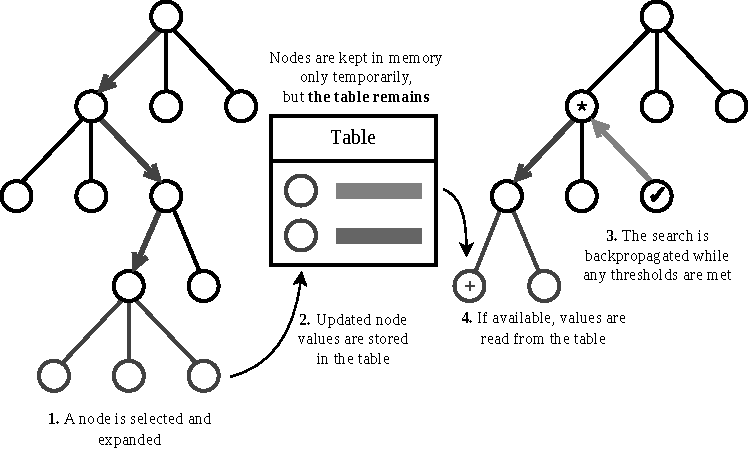
\includegraphics{figures/MemoryVisualizedDfBstarMono.pdf}
    \else
        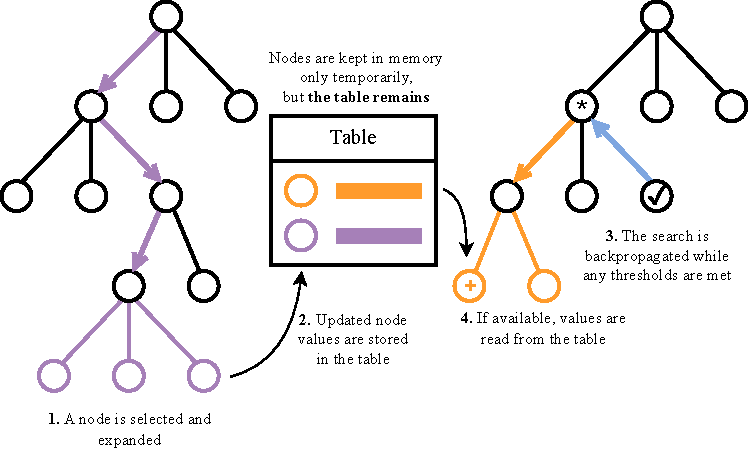
\includegraphics{figures/MemoryVisualizedDfBstar.pdf}
    \fi
    \caption{This diagram depicts how memory is handled in df-B* search. Only the direct line of ancestors of the current node and their children are stored in memory during the search. Nodes are constantly getting discarded, so their values are stored in a transposition table as the primary information storage of the algorithm. To reduce the loss of computational effort, the search back-propagates less frequently than B* or ${\text{B*}}^2$ do.}
    \label{fig:memory_fig_df_bstar}
\end{figure}

\subsection{Challenges}
\label{subsec:dfBstarChallenges}
For this thesis, df-B* has been implemented as its minimal viable version as tested on the domain of artificial game trees. This subsection discusses some difficulties and challenges that may be encountered when implementing df-B* or when applying df-B* other domains.
% This thesis describes the ${\text{B*}}^2$, ${\text{B*}}^k$, and df-B* techniques, but df-B* has not been implemented in this thesis and is thus not included in the experiments. However, advice for implementation can be provided based on the theory of the technique. In this subsection, we discuss a few difficulties and challenges that may be encountered when implementing df-B*.

\paragraph{Heuristics.} Unlike df-PN, df-B* requires an evaluation function to work, as well as a, possibly heuristic, strategy selection procedure. Both may need to be adjusted for specific domains. The parameters $\epsilon$ and $\sigma$  may also need to be adjusted to work together with the evaluation function as well as with the strategy selection procedure. Preliminary experiments showed that $\sigma=0.1$ and $\epsilon=0.3$ worked best on the domain of artificial game trees. 
% 
% A note on parameter values: The parameter $\sigma$ may be chosen as $\ge \frac{1}{2}$, but this requires an additional condition for back-propagating the search. If $\sigma \ge \frac{1}{2}$, it is possible that $t \ge \tau$. This could lead to a situation where $\tau \le L < U \le t$. In this scenario, neither threshold can be reached until $L=U$. An additional stop-condition (``$\tau\le L$ \textbf{and} $U \le t$'') can be added to the MID procedure on lines \ref{lst:MIDstopConditionList1} and \ref{lst:MIDstopConditionList2} of Algorithm \ref{alg:MIDdfBstar} to remedy this.

\paragraph{Replacement Schemes.}
The pseudocode given in the previous subsection makes use of a transposition table (TT), which requires a replacement scheme for different-node collisions \cite{Nagai2002}.
Let $n$ be the node to save to the TT, and $m\neq n$ be a node with the same key in the TT, that has been stored earlier.
Our default replacement scheme for df-B*, in this thesis, is to always replace $m$ with $n$. However, this may not be optimal.
Other possible replacement schemes for df-B* may prioritise saving the node that is more likely to be reused, or saving the node that required the most effort to compute. Because df-B* does not search the tree with depth limits, a measure like maximum search depth is not very informative here. It may be better to use the total number of expansions or the size of the frontier as a measure of effort expended. However, the depth of a node can instead be used to determine how likely it is to be reused, as lower-depth nodes are closer to the root and may be checked more frequently.
However, a specific difficulty with depth-first traversing B* is that we cannot determine, based on a TT entry alone, whether $m$ is still globally relevant to the search or not. Even if we know that $m$ required more effort to compute than $n$, it can still be better to save the less costly node $n$, especially if $m$, or one of its ancestors, has since become irrelevant to the search. The simplest solution is therefore to always replace $m$ with $n$, which is what we apply in this thesis.

\paragraph{Note on Transpositions.}
\label{subsec:dfBstarChallenges:Transpositions}
The best-first search methods B* and ${\text{B*}}^2$ are effective for searching on game trees, because they store the game tree in memory directly. However, many games have a natural structure which does not follow a tree. Rather, the structure of many games is that of a directed, often acyclic, graph (DAG).
This means that, when structuring the game as a tree, the same position may be represented multiple times throughout, which we refer to as transpositions of the same game position. This usually results in additional search effort, exploring the same nodes multiple times, even if none are discarded during the search.
On the contrary, df-B* is a depth-first search technique utilising a transposition table, which, as the name suggests, allows df-B* to store transpositions of game positions more efficiently \cite{Nagai2002}. However, the domain we apply in this thesis does not include any transpositions (see Section \ref{sec:AGTmodel}). As a result, df-B* may be shown to perform better, relative to B* and ${\text{B*}}^2$, on other domains.

\paragraph{On the Consideration of Bounds.}
The node selection for B* follows best-first logic based on evaluation function values, which are not always equally informative. For df-PN, the next node selected is always the node with the best lower bound for the amount of work needed to complete the search. The selected node in B* is not exactly a parallel for the most-proving node in PNS, as B* does not propagate information about required effort or work to the top of the tree. The result is that the node selected by B*, and by extension df-B*, is not the node that would lead to the fastest proof overall, as opposed to df-PN \cite{Nagai2002}. \citeA{Palay1983} realised this problem and noted that future research should develop a measure for the amount of work to be done in subtrees to enhance node selection for PB*. Such a measure would benefit the node selection of df-B* as well, and is an interesting candidate for future research.

\paragraph{Final Note on Precision.}
When implementing df-B* to the domain of artificial game trees, we had to consider the precision of the evaluation function supplied to df-B*. For evaluation functions with low granularity, relative to the size of the game tree, B* may have the tendency to spend a lot of search effort in very deep sub-trees. This is a result of the problem discussed in the previous paragraph. However, this tendency is heightened by df-B*, as it may keep searching a branch even after its root values have changed. To counteract this, we increased the Initial Range $R$ (see Section \ref{sec:AGTparams}) of our artificial game trees to provide higher granularity, and thus more precision, to the evaluation function values. Therefore, we advice the use of evaluation functions with high precision to reduce this effect, wherever possible.
% The introduction of the $t$ and $\tau$ thresholds may lead to a more natural implementation for such a measure to improve df-B* overall.

% \paragraph{Final note on Bounds Update.}
% Finally, when implementing the bounds update in lines \ref{lst:MIDupdateBoundsMin} and \ref{lst:MIDupdateBoundsMax} of Algorithm \ref{alg:MIDdfBstar}, there may be some flexibility in implementation. When the bounds of a parent $n$ are loaded from the TT, but those of its children are not, then updating $L$ and $U$ of $n$ may result in wider bounds. This can result in fewer prunings during the search. To avoid this, we can keep the loaded bounds of $n$ in memory and use them to prune nodes until better bounds are computed. Alternatively, the bounds update could be altered such that $L$ and $U$ of $n$ only get modified if the new values are better (higher $L$ and lower $U$). This modification has not been tested in our experiments on B* or ${\text{B*}}^2$, so the effects of this change may be adverse. It is therefore not included in the description of df-B*, but might improve performance if implemented.
%
% If the bounds $L,U$ of $n$ are saved in the TT, but the children of $n$ were not, then $U'-L'$ might end up being $> U-L$, which is not desired behaviour. To reduce this, ensure that nodes are pruned (discarded) before the bounds of $n$ are updated.
%
% Additionally, one could implement that bounds do not update if they do not improve, that is, $L\coloneqq\max\left[L_{old}, L_{new}\right]$ and $U\coloneqq\min\left[U_{old}, U_{new}\right]$. This may result in earlier prunings of some nodes. This modification has not been tested in our experiments on B* or ${\text{B*}}^2$, so the effects of this change may be adverse. It is therefore not included in the description of df-B*, but might improve performance if implemented.

\chapter{Artificial Game Trees}
\label{cht:ArtificialGameTrees}
Search techniques are often applied to games in research due to the advantages that a game environment provides. The implementation of search techniques in a specific game environment may still require some additional complexity, however. This is especially the case when strong heuristics are required for algorithms to perform well in the chosen environment. The techniques being explored in this thesis are heuristic-dependent, so picking the right environment is important for a fair comparison of methods. We therefore apply the domain of Artificial Game Trees (AGTs) described by \citeA{Berliner1979}, and later adapted by \citeA{Anema2025}. 

The structure of this chapter is as follows. First Section \ref{sec:AGTorigin} describes the existing literature we build on for our implementation of AGTs. Second, Section \ref{sec:AGTmodel} defines the domain of AGTs as it is applied in this thesis. Finally, Section \ref{sec:AGTparams} gives an overview of the parameters controlling the structure and generation of AGTs.

\section{Origin}
\label{sec:AGTorigin}
As opposed to testing the performance of our search techniques on a game environment, we do so on a computer-generated set of problems in the form of AGTs. Our implementation of AGTs is based on the description by \cite{Anema2025}, which is based on the description by \citeA{Berliner1979}.

\paragraph{\texorpdfstring{\protect\citeA{Berliner1979}}{Berliner (1979)}}
described the generation of canonical AGTs for the evaluation of the B* search technique. These trees were expanded during the search, and form the same structure regardless of the order in which the tree is explored. This was achieved by assigning a unique name and corresponding seed $S_n$ to each node based on its position. Node values were generated such that expansion only ever tightens the bounds of node, as was required for B*. As a result, each tree has a unique solution and could potentially be infinitely large. Two parameters control the structure of the tree: the width, or branching factor, $b$, and the range $R$. However, these trees are all quite similarly structured, and the parameters do not allow for a lot of control.

\paragraph{\texorpdfstring{\protect\citeA{Anema2025}}{Anema (2025)}}
expanded on this model to evaluate B* and Disprove-Best B* on larger and more varied trees. These trees were generated in the same way as by \cite{Berliner1979}, but include two additional parameters: the distribution parameter $k$, and the growth factor $g$. This allowed for more control on the structure and size of the AGTs. The AGTs we describe in this thesis are based on the \textit{AdjustAfter} variant as described by \citeA{Anema2025}. However, we redefine how the seeds $S_n$ for nodes are chosen and introduce another parameter: the relevance chance $r$.

\section{Description}
\label{sec:AGTmodel}
This section describes how AGTs are initialised and constructed in this thesis. The section is structured as follows. First Subsection \ref{subsec:AGTseeds} describes how we generate canonical AGTs, and how this differs from previous work. Second and finally, Subsection \ref{subsec:AGTgeneration} describes the generation of AGTs with corresponding pseudocode.

\subsection{Seeds for Canonical Trees}
\label{subsec:AGTseeds}
For the generation of canonical trees, \citeA{Berliner1979} assigned names to nodes in the tree based on their position. This approach assumes the tree has a fixed or maximum Branching Factor $b$. If we assign the name `0' to the root node, the name of a node $n$ with parent $p$ is chosen as:
\begin{gather}
    \text{name}\left(n\right) = b\cdot \text{name}\left(p\right) + i
    \label{eq:AGT:nodeName}
\end{gather}
where $i=1,\dots,b$ is the index of $n$ within the list of children of $p$. All generated values, centred on $n$, are then determined with a pseudorandom number generator (RNG) with a seed based on the name of $n$. The modification we introduce is in how this seed is chosen. The novel idea is the Initial Seed parameter $S_0$ and the node-specific seed $S_n$ computed as:
\begin{gather}
    S_n = \text{name}\left(n\right) + \left(\text{name}\left(n\right) + 1\right) \cdot S_0
\end{gather}
where the Initial Seed $S_0$ is a tree parameter which is best chosen as a large random 64-bit integer not equal to 0. Conceptually, $S_0$ is not only the tree specific seed, but also the node-specific seed $S_{n_0}$ of the root node $n_0$ where $\text{name}\left(n_0\right)=0$. We found that this approach resulted in fewer overlapping seeds than the approach described by \cite{Berliner1979}.

\subsection{Node Generation}
\label{subsec:AGTgeneration}
As described by \citeA{Berliner1979} and \citeA{Anema2025}, only the root node $n_0$ of a tree $T$ is provided initially, and the rest of the tree is generated dynamically. We apply the generation step for AGTs at the `compute all possible moves' step of the search, which we refer to as node expansion. For every node expansion of any node $n$, it is ensured that if the bounds of $n$ are updated after expansion, that they (a) never get wider, and (b) always have a non-zero chance to shrink.

\paragraph{Relevance Chance.} The procedure for generating nodes is mostly identical to the \textit{AdjustAfter} procedure described by \citeA{Anema2025}.
However, we introduce a minor modification. The novel idea is the introduction of the Relevance Chance parameter $r$, which relates to how children are generated when the Growth Factor $g$ is greater than 1. Without $r$ ($r=0$), a large growth factor does not strictly increase the size of the tree, but may also decrease it. Children can be generated outside of the bounds of their parent, which makes them immediately irrelevant to the search.
The Relevance Chance $r$ is the chance of randomly forcing a node to be relevant to the search. This is applied to every generated node, and may have no effect if the node had already been relevant before.
Preliminary experiments showed that, if $g\gg 1$ and $k$ is relatively large, then $r$ has a very strong effect on the size of the tree, with values closer to 1 making the tree increasingly harder to solve.
\newpage
\paragraph{Pseudocode.} The pseudocode of Algorithm \ref{alg:AGT} details the procedure of generating the children $c_1,\dots,c_b$ of the node $n$ given the tree-specific parameters $S_0$, $b$, $k$, $g$, and $r$. The Initial Range parameter $R$ is defined as the initial upper bound of the root node $n_0$, where the lower bound is set to $0$. Additionally, trees may be generated as adversarial or non-adversarial, where non-adversarial trees only have maximising nodes, and adversarial trees alternate between maximising and minimising nodes by depth. The root node $n_0$ is always maximising.
Finally, as described by \citeA{Berliner1979}, the lower and upper bounds of all nodes are represented by integer values, so a node can be generated as a terminal node if its lower bound is equal to its upper bound.

\vspace{4ex}

\begin{algorithm}[hbtp]
\begin{algorithmic}[1]
	\State \textbf{if} Lower($n$) = Upper($n$) \textbf{then} \Return $\emptyset$
    \State \textbf{set seed} $S_n\coloneqq \text{Name}\left(n\right) + \left(\text{Name}\left(n\right) + 1\right) \times S_0$ \Comment{``$\sim_n$'' indicates use of this generator}
    \ForAll{$i$ in $1,\dots,b$}
        \State L $\coloneqq$ Lower($n$)
        \State U $\coloneqq$ Upper($n$)
        \State $\Delta \coloneqq \left(g - 1\right) \times \left(U - L\right)$
        \State $D \coloneqq \lfloor\Delta\rfloor + I\sim_n I\in\left\{0,1\right\}~s.t.: \mathbb{E}\left(D\right)=\Delta$
        \Comment{gives $\Delta\in\mathbb{R}$ and $D\in\mathbb{Z} \approx \Delta$}

        \If{isMaximising($n$)}
            \State $v_1,\dots,v_k \sim_n\mathcal{U}\left\{L-D, U\right\}$
        \Else
            \State $v_1,\dots,v_k \sim_n\mathcal{U}\left\{L, U+D\right\}$
        \EndIf
        \If{$g > 1$ \textbf{and} $r > X\sim_n\mathcal{U}\left[0,1\right)$}
            \State $v_{k+1} \sim_n\mathcal{U}\left\{L, U\right\}$
        \EndIf
        \State $c_i \coloneqq$ child of $n$ where:
        \State ~~isMaximising($c_i$) $\coloneqq$ \textbf{not} isMaximising($n$) \Comment{\textbf{if} tree is non-adversarial \textbf{then} $\coloneqq$ `yes'}
        \State ~~Name($c_i$) $\coloneqq$ Name($n$)$~\times~b + i$
        \State ~~Lower($c_i$) $\coloneqq \min_j v_j$
        \State ~~Upper($c_i$) $\coloneqq \max_j v_j$
    \EndFor
    \If{$\min_i \left[\text{Lower}\left(c_i\right)\right] < \text{Lower}\left(n\right)$ \textbf{or} $\max_i \left[\text{Upper}\left(c_i\right)\right] > \text{Upper}\left(n\right)$}
    \State $\ell \sim_n \mathcal{U}\left\{1,b\right\}$
    \State $v_1',\dots,v_k' \sim_n \mathcal{U}\left\{L,U\right\}$
    \State Lower($c_\ell$) $\coloneqq \min_j v_j'$
    \State Upper($c_\ell$) $\coloneqq \max_j v_j'$
    \EndIf
\end{algorithmic}
\caption{Expand($n$, $S_0$, $b$, $k$, $g$, $r$) $\to c_1,\dots,c_b$; the children of $n$}
\label{alg:AGT}
\end{algorithm}
\paragraph{Note on Transpositions.}
AGTs, as described in this chapter, differ from natural game trees in the presence of transpositions. Natural game trees often have an underlying structure that does not match an actual tree, but is rather a directed, and often acyclic, graph (DAG). This allows for multiple paths to reach the same node, referred to as a transposition. However, AGTs are strictly trees, with effectively no transpositions at all. This has no significant effect on search techniques that assume the game is strictly a tree. Although this may increase the relative difficulty of trees for techniques designed for DAGs. This includes depth-first search utilising transposition tables, like df-B* described in Section \ref{sec:dfBstar}, but excludes the best-first search techniques B* and ${\text{B*}}^2$.
% In game tree search, these transpositions may cause problems, as the tree structure of the search makes the problem appear larger than it is, sometimes requiring the search to explore the same position multiple times because of transpositions.
% While artificial game trees are constructed to be relatively varied and may require substantial search effort to solve, they have a clear distinction from natural game trees.

\newpage
\section{Parameter Overview}
\label{sec:AGTparams}
This section provides an overview of all tree-specific parameters for the generation of AGTs as described in this thesis. Table \ref{tab:AGTparams} lists all tree-specific parameters and their description. Table \ref{tab:AGTparamsComplex} lists the possible and recommended values for each parameter, and the expected effect of each parameter on the complexity of the tree. In this context, complexity refers to the number of node expansions needed, on average, by B* to solve the resulting trees.

\begin{table}[htbp]
\centering
\begin{tabular}{lll}
\textbf{Parameter}  & & \textbf{Description}                                                \\ \hline
Adversarial         &       & Alternates maximising and minimising nodes                          \\ \hline
Initial Seed        & $S_0$ & Determines the result of random outcomes                            \\ \hline
Initial Range       & $R$   & Initial upper bound of the root, with a lower bound of 0 \\ \hline
Branching Factor    & $b$   & Number of children generated at every internal node             \\ \hline
Distribution Factor & $k$   & 
    \begin{tabular}[c]{@{}l@{}}Number of $v_1,\dots,v_k$ considered for the generation of the bounds\\ of a node where $Low(n) = \min_i\left(v_i\right)$ and $Upp(n) = \max_i\left(v_i\right)$ \end{tabular} \\ \hline
Growth Factor       & $g$   & Ratio of maximum allowed child range to parent range \\ \hline
Relevance Chance    & $r$   &
  \begin{tabular}[c]{@{}l@{}}Chance to generate an extra $v_{k+1}$ of child within parent range\\ which forces the child to be relevant to the search\end{tabular}
\end{tabular}
\caption{Parameters for the generation of artificial game trees, and their description.
The additional value generated by the relevance chance $r$ is on top of the number of values generated as determined by $k$. Therefore, the effective $k$ (\# values considered for bounds) is $k+r$.}
\label{tab:AGTparams}
\end{table}

\begin{table}[htbp]
\centering
\begin{tabular}{lllll}
\textbf{Parameter} &
  \multicolumn{1}{c}{\textbf{}} &
  \textbf{\begin{tabular}[c]{@{}l@{}}Possible\\ Values\end{tabular}} &
  \textbf{\begin{tabular}[c]{@{}l@{}}Recommended\\ Values\end{tabular}} &
  \textbf{\begin{tabular}[c]{@{}l@{}}Effect on\\ Complexity\end{tabular}} \\ \hline
Adversarial         &       & yes, no                  & any              & uncertain \\ \hline
Initial Seed        & $S_0$ & 64-bit integers          & randomised, $\neq 0$  & none      \\ \hline
Initial Range       & $R$ & $n \ge 1 \in \mathbb{N}$ & $10^2$ to $10^9$ & uncertain \\ \hline
Branching Factor    & $b$   & $n \ge 2 \in \mathbb{N}$ & $2$ to $100$     & low       \\ \hline
Distribution Factor & $k$   & $n \ge 2 \in \mathbb{N}$ & $2$ to $20$      & high      \\ \hline
Growth Factor &
  $g$ &
  $x > 0 \in \mathbb{R}$ &
  \begin{tabular}[c]{@{}l@{}}$\ge 1$\\ $< 1$ shrinks tree\end{tabular} &
  \begin{tabular}[c]{@{}l@{}}depends on $k$ and $r$\\ negative (if $< 1$)\end{tabular} \\ \hline
Relevance Chance &
  $r$ &
  $x \in \left[0,1\right]$ &
  \begin{tabular}[c]{@{}l@{}}$<1$, if $g\gg 1$\\ any, otherwise\end{tabular} &
  \begin{tabular}[c]{@{}l@{}}very high (if $g\gg 1$)\\ none (if $g\le 1$)\end{tabular}
\end{tabular}
\caption{Parameters for the generation of artificial game trees and their effects on the complexity (\# nodes needed to solve problem) of the trees generated. 
Positive effect means increasing this parameter increases the complexity of the tree. The growth factor $g$ has a high effect if $k$ is also chosen to be large, and 
a negative effect if $g \gg 1$ while $r \approx 0$ and $k$ is small.}
\label{tab:AGTparamsComplex}
\end{table}


\chapter{Experiments and Results}
\label{cht:Experiments}
This chapter describes the performed experiments and their results, and is structured as follows.
Section \ref{sec:ExpSetup} describes the experimental setup, including hardware specifications, a list of terms, and experimental details of two experiments. Section \ref{sec:Results} presents the experimental results.

\section{Experimental Setup}
\label{sec:ExpSetup}
This section describes the experiments that were performed for this thesis. First, hardware and software specifications for the experiments are provided in Subsection \ref{subsec:Hardware}. Second, a list of terms is provided in Subsection \ref{subsec:ExpTerms}. Third, Subsection \ref{subsec:Exp1} describes Experiment\ 1. Finally, Subsection \ref{subsec:Exp2} describes Experiment\ 2.

\subsection{Hardware Specifications}
\label{subsec:Hardware}
The code for all search techniques, artificial game trees, and experiments was written and executed in Java 17. The individual runs of all experiments were run in parallel, with up to 32 runs computed simultaneously, on an AMD 5950X CPU with 64GB of DDR4 RAM running Windows 11. All runtime measurements were performed with the \texttt{java.time.Instant.now()} and \texttt{java.time.Duration.toNanos()} methods.

\subsection{List of Terms}
\label{subsec:ExpTerms}
We define the following terms to describe the experimental methodology.

\paragraph{Tree}
refers to an Artificial Game Tree (AGT), as described in Chapter \ref{cht:ArtificialGameTrees}, which is uniquely defined by its parameters. The Initial Seed parameter $S_0$ is set to a unique value for each tree, as it determines the seeds of the pseudo-random number generators used to generate the tree structure.
\paragraph{Initialisation}
refers to the construction of the root of a tree, which is defined by its parameters. This tree can then be expanded indefinitely using any B* search technique to compute its solution.
\paragraph{Solution}
refers to the next best move, or `best node', as computed from the root of a tree. The solution of each tree is not known in advance, but can be computed through B* search. A solution is found and proven whenever separation \cite{Berliner1979} is reached at the root of the tree. Separation occurs when, assuming a node is maximising (without loss of generality), the lower bound of the best node exceeds or equals the upper bound of all alternative nodes. As an additional check, the solutions of all solved runs were cross-referenced with each other per tree, which confirms that all algorithms arrived at the same unique solution for each tree.
\paragraph{Run}
refers to, given a tree $T$ and some B* search technique $B$, the process of computing the solution of $T$ using $B$. A run may be restricted by an expansion limit and a node limit, which each may cause the run to terminate early. A run will be marked as solved if a solution was found and proven; this can also happen when a run was terminated early. The results of a run additionally include several metrics which are recorded during the search.
\paragraph{Metrics}
refers to the measurements made for the experiments, which are recorded during runs. Given a run of some tree $T$ and some search technique $B$, we determine the following metrics:
\begin{itemize}
    \item \textbf{Expansion} occurs whenever $B$ selects the next node $n$ of $T$ for which the children of $n$ are not accessible to $B$. `Expansions' or `Number of Nodes Expanded' refers to the total number of expansions during the run. Expansion is the metric which considers the cost of computing the children of a node $n$. The children of $n$ may have been computed before, but not be accessible to $B$, if they have been previously removed from memory.
    \item \textbf{Nodes} are the core representation of game positions of $T$ during the search. The metric `nodes' or `maximum nodes' refers to the maximum number of nodes held in memory by $B$ during the run. Nodes are recorded differently for df-B*, as its transposition table takes up constant memory. We measure the number of nodes for df-B* as the maximum number of nodes held in its execution stack during the run.
    \item \textbf{Time} is the number of seconds that have passed from the start of the run to its termination. The preparation time for initialising $T$ and $B$ is excluded. Preparation time for search techniques includes the creation of transposition tables for df-B*.
\end{itemize}
\paragraph{Expansion limit}
refers to an artificial limit imposed on each run to control the total runtime of the experiment. The expansion limit is an additional stop condition which terminates a run early when the number of expansions exceeds the specified limit. The expansion limit is described as the maximum number of expansions performed during a single run.
\paragraph{Node limit}
refers to an artificial limit imposed on a run to control the amount of memory available to the search. The node limit is an additional stop condition which terminates a run early when the number of nodes in memory exceeds the specified limit. The node limit is described as the maximum number of nodes held in memory during a run.

\subsection{Experiment 1: General Comparison}
\label{subsec:Exp1}
This subsection describes the first experiment, which is aimed at providing a general comparison of B*, ${\text{B*}}^2$, and df-B* on the domain of artificial game trees. We performed 10 runs with two variants of B*, 10 runs with two variants of ${\text{B*}}^2$, and 3 runs with two variants of df-B* on each of 25\thsep920 unique trees, for a total of 1\thsep192\thsep320 runs. The experiment is described in the following order. First, the included algorithm variants are described. Second, the experimental set of trees is described. Finally, the imposed expansion limits and node limits are described.

\paragraph{Algorithm Variants.}
\label{subsec:Exp1:Algorithms}
Experiment\ 1 includes two variants of B*, two variants of ${\text{B*}}^2$, and two variants of df-B*. These variants have been implemented as follows:
\begin{enumerate}
    \item \textbf{B*} is a modified B* \cite{Berliner1979} implementation as described in Section \ref{sec:BstarAdjustments:Modifications}. The strategy selection of B* is performed with the $A$\textbf{R-criterium} as described in Subsection \ref{subsec:strategySelection:Heuristic}, where $A$ refers to considering all alternatives in the calculation of the strategy.
%
    \item \textbf{B*-alt} is mostly the same as \textbf{B*} described above. However, the strategy selection is instead performed with the \textbf{Alternated} method, as described in Subsection \ref{subsec:strategySelection:Naive}.
%
    \item \textbf{B*}$^2$ is as described in Section \ref{sec:BstarSquared}, with the following parameters. The first-level search is performed with \textbf{B*}. The second-level search is performed with \textbf{B*-alt}. The size limits of the second-level tree are determined by a logistic growth function, as described in Subsection \ref{subsec:Level2SizeLimit:Sigmoid}, where $a=5\cdot10^5$ and $b=5\cdot10^4$. The second-level search uses the stop conditions \textbf{separation} and \textbf{size limit} (see Subsection \ref{subsec:BstarSquaredAlgorithm:StopConditions}) and applies the \textbf{full disposal} approach for bounds preservation (see Subsection \ref{subsec:BstarSquaredAlgorithm:BoundsPreservation}).
%
    \item \textbf{B*}$^2$\textbf{-alt} is mostly the same as \textbf{B*}$^2$ described above, with the following differences. The first-level search is performed with \textbf{B*-alt}. The second-level search uses \textbf{Always-PB} (see Subsection \ref{subsec:strategySelection:Naive}) for strategy selection.
%
    \item \textbf{df-B*} is as described by Algorithm \ref{alg:dfBstar} and Section \ref{sec:dfBstar}. The df-B*-specific thresholding parameters are chosen as $\sigma=0.1$ and $\epsilon=0.3$. Strategy selection is performed with the $A$\textbf{R-criterium}, same as \textbf{B*}. An initial maximum depth of $10$ is applied to the search, which is incremented by $1$ every time it is exceeded. Upon reaching the maximum depth, the search is forcibly backed up to the root. As an implementation detail, the search may also be forced to back up to the root if some operation-system-dependent stack-size limit is exceeded. Upon which the stack-size limit is doubled, and the search is resumed.
%
    \item \textbf{df-B*-alt} is mostly the same as \textbf{df-B*} described above. However, the strategy selection is instead performed with the \textbf{Alternated} method, as described in Subsection \ref{subsec:strategySelection:Naive}.
%
\end{enumerate}

\paragraph{Trees.}
\label{subsec:Exp1:Trees}
Experiment\ 1 is performed on a diverse set of artificial game trees. The trees for this experiment were initialised with all combinations of the parameter values shown in Table \ref{tab:TreeParamsExp1}, for a total of $6\cdot3\cdot6\cdot6=648$ tree variants.
We did not include non-adversarial trees in the experiment, because their inclusion resulted in much smaller trees, which did not contribute much to the overall results.
For each tree variant, we initialised 40 unique trees by applying a different Initial Seed $S_0$ (see Table \ref{tab:AGTparams}) to each tree, for a total of $648\cdot40=\text{25\thsep920}$ trees. The details of seed allocation are described in Section \ref{sec:SeedAllocationExp1} in the Appendix. The choice of seeds ensures that every tree is an independent problem with a unique solution.

\begin{table}[ht]
\centering
\begin{tabular}{lc|l}
\multicolumn{2}{l|}{\textbf{Parameter}} & \textbf{Assigned Values} \\ \hline
Adversarial         &     & yes \\
Initial Range       & $R$ & 10\thsep000\thsep000 \\
Branching Factor    & $b$ & $2,\ 3,\ 5,\ 10,\ 15,\ 30$\\
Distribution Factor & $k$ & $4,\ 5,\ 6$ \\
Growth Factor       & $g$ & $1,\ 1.1,\ 1.2,\ 1.3,\ 1.4,\ 1.5$ \\
Relevance Chance    & $r$ & $0,\ 0.2,\ 0.3,\ 0.4,\ 0.5,\ 0.6$
\end{tabular}
\caption{List of parameter values for the 648 different tree variants included in Experiment\ 1. See Table \ref{tab:AGTparams} and Chapter \ref{cht:ArtificialGameTrees} for the definitions and use of these parameters, and see Section \ref{sec:SeedAllocationExp1} for details on how the Initial Seed parameter $S_0$ was assigned for this experiment.}
\label{tab:TreeParamsExp1}
\end{table}

\paragraph{Imposed Limitations.}
Each of the 1\thsep192\thsep320 runs was performed with an expansion limit of 5\thsep000\thsep000 and a node limit of $2^{20}=\text{1\thsep048\thsep576}$. This node limit was realised for df-B* through the use of a transposition table of size $2^{20}$ (Subsection \ref{subsec:dfBstarChallenges}). The index for the transposition table of any node $n$ from the artificial game tree is chosen as the 20 rightmost bits of a pseudo-randomly generated 64-bit value, seeded with the node-specific seed $S_n$ (Section \ref{sec:AGTmodel}).

\FloatBarrier
\subsection{Experiment 2: Memory Usage}
\label{subsec:Exp2}
This subsection describes the second experiment, which explores the memory footprint of ${\text{B*}}^2$ compared to B* by conducting runs with various node limits.
The experimental setup was fine-tuned based on the results of Experiment\ 1.
We performed 25 runs with two variants of ${\text{B*}}^2$ and 10 runs with one variant of B* on each of 12\thsep000 unique trees, for a total of 720\thsep000 runs. The experiment is described in the following order. First, the included algorithm variants are described. Second, the experimental set of trees is described. Finally, the imposed expansion limits and node limits are described.

\paragraph{Algorithm Variants.}
\label{subsec:Exp2:Algorithms}
Experiment\ 2 includes one variant of B* and two variants of ${\text{B*}}^2$. df-B* was not included in this experiment due to time constraints. However, its memory footprint is already well enough understood from the results of Experiment\ 1. The selected algorithm variants have been implemented as follows:
\begin{enumerate}
    \item \textbf{B*} is the default B* implementation we describe for Experiment\ 1 in Subsection \ref{subsec:Exp1:Algorithms}.
    \item \textbf{B*}$^2$ is the default ${\text{B*}}^2$ implementation we describe for Experiment\ 1 in Subsection \ref{subsec:Exp1:Algorithms}.
    \item \textbf{B*}$^2$\textbf{-max} is mostly the same as \textbf{B*}$^2$. However, the second-level search is performed with a more lenient tree-size limit. Instead of a logistic growth function, the size of the second-level tree is limited only by the current size of the first-level tree (see Subsection \ref{subsec:Level2SizeLimit}).
\end{enumerate}
Other variants from Experiment\ 1, \textbf{B*-alt} and \textbf{B*}$^2$\textbf{-alt}, were not included because their performance was too similar to \textbf{B*} and \textbf{B*}$^2$, based on the results of Experiment\ 1. \textbf{B*}$^2$\textbf{-max} was included because its memory footprint differed greatly from \textbf{B*}$^2$ in preliminary experiments.

\paragraph{Trees.}
\label{subsec:Exp2:Trees}
The artificial game trees for this experiment were selected based on the results of Experiment\ 1. Trees were initialised with all combinations of the parameter values shown in Table \ref{tab:TreeParamsExp2}, for a total of $3\cdot2\cdot4=24$ variants.
These variants were chosen as a subset of the 648 tree variants of Experiment\ 1 with roughly the highest proportion of trees requiring more than 50\thsep000 node expansions but not exceeding the node or expansion limits. 
For each tree variant, we initialised 500 unique trees by providing a different Initial Seed $S_0$ (see Table \ref{tab:AGTparams}) to each tree, for a total of $24\cdot500=\text{12\thsep000}$ trees. Seeds are chosen such that none overlap with the seeds for Experiment\ 1.
Further details of seed allocation are shown in Table \ref{tab:SeedAllocationExp2} in the Appendix. The choice of seeds ensures that every tree is an independent problem with a unique solution.

\begin{table}[ht]
\centering
\begin{tabular}{lc|l}
\multicolumn{2}{l|}{\textbf{Parameter}} & \textbf{Assigned Values} \\ \hline
Adversarial         &     & yes \\
Initial Range       & $R$ & 10\thsep000\thsep000 \\
Branching Factor    & $b$ & $5,\ 10,\ 15$\\
Distribution Factor & $k$ & $5,\ 6$       \\
Growth Factor       & $g$ & $1.2,\ 1.3,\ 1.4,\ 1.5$ \\
Relevance Chance    & $r$ & $0.4$
\end{tabular}
\caption{List of parameter values for the $24$ different tree variants included in Experiment\ 2. See Table \ref{tab:AGTparams} and Chapter \ref{cht:ArtificialGameTrees} for the definitions and use of these parameters, and see Table \ref{tab:SeedAllocationExp2} for details on how the Initial Seed parameter $S_0$ was assigned for this experiment.}
\label{tab:TreeParamsExp2}
\end{table}

\paragraph{Imposed Limitations.}
Unlike B*, ${\text{B*}}^2$ behaves differently depending on the node limit. ${\text{B*}}^2$ increasingly restricts the extent of its second-level searches as the first-level tree approaches the overall node limit. Therefore, we select various node limits to more precisely measure the memory requirements of ${\text{B*}}^2$. The 25 different node limits applied to \textbf{B*}$^2$ and \textbf{B*}$^2$\textbf{-max} are listed in Table \ref{tab:nodeLimitsExp2}. For all B* runs, we apply the same node limit of 15\thsep000\thsep000. All runs also had an expansion limit of 10\thsep000\thsep000.

% All runs of \textbf{B*}$^2$ and \textbf{B*}$^2$\textbf{-max} were performed with one of 25 different node limits, as listed in Table \ref{tab:nodeLimitsExp2}.
% The 25 different node limits applied to both ${\text{B*}}^2$ variants are listed in Table \ref{tab:nodeLimitsExp2}.
% , we apply one of 25 different node limits to each run of \textbf{B*}$^2$ or \textbf{B*}$^2$\textbf{-max}.
% The ${\text{B*}}^2$ runs were each performed with a limit of 10\thsep000\thsep000 expansions and one run for each of the 25 different node limits listed in Table \ref{tab:nodeLimitsExp2}. The B* runs were each performed with a limit of 10\thsep000\thsep000 expansions and a node limit of 15\thsep000\thsep000.
\begin{table}[ht]
\begin{tabular}{lllllllll}
5 & 10 & 25 & 50 & 100 & 200 & 500 & 1000 & 2000 \\
5000 & 10\thsep000 & 15\thsep000 & 20\thsep000 & 50\thsep000 & 75\thsep000 & 115\thsep000 & 150\thsep000 & 200\thsep000 \\
275\thsep000 & 350\thsep000 & 450\thsep000 & 600\thsep000 & 700\thsep000 & 850\thsep000 & 1\thsep000\thsep000 & &
\end{tabular}
\caption{List of 25 node limits applied to the ${\text{B*}}^2$ runs of Experiment\ 2.}
\label{tab:nodeLimitsExp2}
\end{table}

\section{Results}
\label{sec:Results}
This section describes the results from the experiments described in Section \ref{sec:ExpSetup}.
All intervals shown in this section, denoted by `$\pm$', are 95\% confidence intervals rounded to two significant digits.
Additionally, all averages shown are rounded to the same decimal place as their interval half-widths.
% with half-widths rounded to two significant digits. Additionally, all averages are rounded to the same level of precision as
% All averages shown in this section were rounded to the order of magnitude of their 95\% confidence interval half-width.
This section is structured as follows.
Subsection \ref{subsec:ResultsExp1} shows the results from Experiment 1. Subsection \ref{subsec:ResultsExp2} shows the results from Experiment 2.
\subsection{Experiment 1}
\label{subsec:ResultsExp1}
The results from Experiment\ 1 include the recorded metrics of 1\thsep192\thsep320 runs on 25\thsep920 trees, which were performed as described in Subsection \ref{subsec:Exp1}. Recorded metrics include the number of expansions, the number of nodes, and the duration of runs, as defined in Subsection \ref{subsec:ExpTerms}. Additionally, each run was recorded as `solved' if separation was reached, and as `unsolved' otherwise. In total, 1\thsep005\thsep723 runs were marked as solved, which accounts for 23\thsep521 trees. Out of these trees, 15\thsep131 trees were solved by all algorithm variants in all runs, which we refer to as `the set of \textbf{universally solved trees}'. Figure \ref{fig:Exp1SolvedPerAlgAllRuns} shows the number of trees solved by each of the six algorithm variants, which shows that \textbf{B*}$^2$ solved the most trees (23\thsep477), and \textbf{df-B*} solved the least trees (15\thsep309). However, this result depends on the choice of expansion and node limits.
If we lower the expansion limit to 1\thsep000\thsep000, then \textbf{B*}$^2$ still solves the most trees (22\thsep724), which is only $0.6\%$ more than B* (22\thsep586), which remains unchanged.
If we instead lower the node limit to 300\thsep000, then \textbf{B*} only solves 21\thsep305 trees, while \textbf{B*}$^2$ remains unchanged.
%
\begin{figure}[htbp]
	\centering
	\ifMonochrome
	
\includegraphics[scale=0.7]
	{figures/graphs/monochrome/fig1SolvedPerAlgAllRuns.pdf}
	\else
	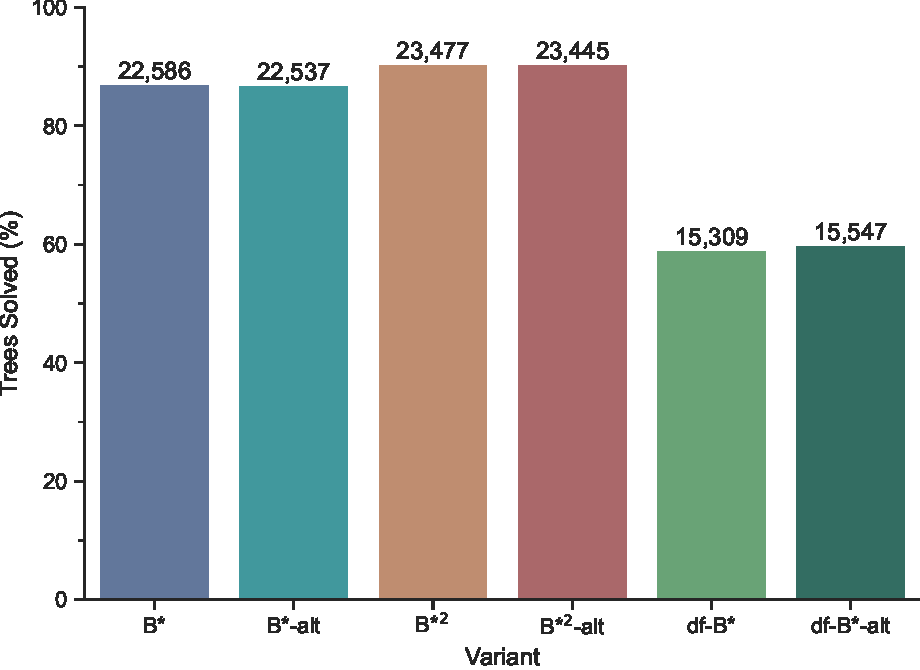
\includegraphics[scale=0.7]
	{figures/graphs/colour/fig1SolvedPerAlgAllRuns.pdf}
	\fi
	\caption{This figure shows the percentage and number of trees, out of 25\thsep920, that were solved at least once, grouped by algorithm variant. The values atop each bar show the exact number of trees, whereas the height of the bar shows the percentage.}
	\label{fig:Exp1SolvedPerAlgAllRuns}
\end{figure}

\paragraph{Efficiency.} We compare the computational efficiency of these algorithm variants by measuring their relative performance on the same set of trees. Figure \ref{fig:Exp1ExpansionsPerAlgSolvedByAll} shows the average number of expansions on the set of 15\thsep131 universally solved trees, grouped by algorithm variant. It is shown that \textbf{df-B*} expands the most nodes
$\left(\approx10\text{\thsep}200\pm2100\right)$,
and \textbf{B*} expands the least nodes
$\left(\approx539\pm23\right)$.
The results show no significant difference between \textbf{B*} and \textbf{B*-alt}
$\left(\approx562\pm24\right)$,
or between \textbf{B*}$^2$
$\left(\approx843\pm35\right)$
and \textbf{B*}$^2$\textbf{-alt}
$\left(\approx854\pm36\right)$.
However, \textbf{df-B*-alt}
$\left(\approx5400\pm1200\right)$
expands significantly fewer nodes than \textbf{df-B*}.
Taking the best result for each of the three B* techniques, we calculate that \textbf{B*}$^2$ expanded on average 56\% more nodes than \textbf{B*}, whereas \textbf{df-B*-alt} expanded on average 902\% more nodes than \textbf{B*}.
% All intervals are $95\%$ confidence intervals.
\begin{figure}[htbp]
	\centering
	\ifMonochrome
	
\includegraphics[scale=0.7]
	{figures/graphs/monochrome/fig1ExpansionsPerAlgSolvedByAll.pdf}
	\else
	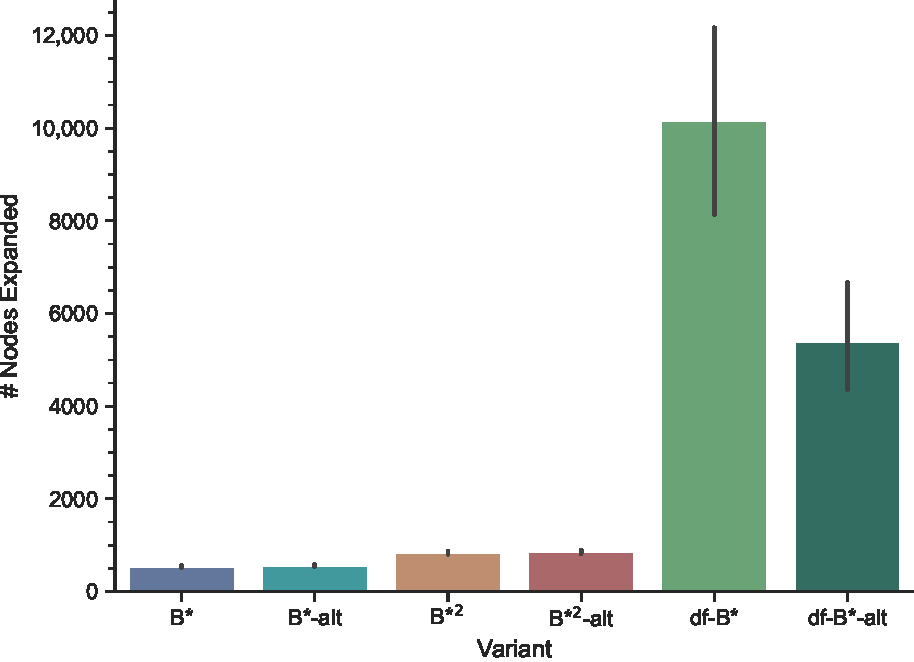
\includegraphics[scale=0.7]
	{figures/graphs/colour/fig1ExpansionsPerAlgSolvedByAll.pdf}
	\fi
	\caption{This figure shows the average number of nodes expanded by each of six algorithm variants on the set of 15\thsep131 universally solved trees. Also shown are $95\%$ confidence intervals.}
	\label{fig:Exp1ExpansionsPerAlgSolvedByAll}
\end{figure}

In addition to the total number of expansions, we compute the number of expansions per second. Figure \ref{fig:Exp1ExpansionsPerSecondAllTrees} shows the average ratio of the number of expansions to the run duration in seconds, grouped by algorithm variant.
These rates were computed on a subset of all 25\thsep920 trees.
Due to an implementation detail, we could not accurately measure the duration of runs shorter than 0.0005 seconds; therefore, all trees with runtimes below 0.0005 seconds were excluded, resulting in 13\thsep936 trees.
The rate of expansion may indicate the level of overhead introduced by the algorithm variant.
The results show that \textbf{B*-alt} has the highest rate of expansion
$\left(\approx205\text{\thsep}390\pm580\right)$,
which is marginally higher than \textbf{B*}
$\left(\approx200\text{\thsep}590\pm560\right)$.
Marginally lower is the expansion rate of \textbf{B*}$^2$
$\left(\approx 194\text{\thsep}630\pm500\right)$,
which is not significantly different from \textbf{B*}$^2$\textbf{-alt}
$\left(\approx195\text{\thsep}600\pm510\right)$.
Finally, \textbf{df-B*}
$\left(\approx36,880\pm260\right)$
and \textbf{df-B*-alt}
$\left(\approx37,750\pm260\right)$
have the lowest rates of expansion. These results indicate that \textbf{B*}, \textbf{B*-alt}, \textbf{B*}$^2$, and \textbf{B*}$^2$\textbf{-max} have a similar amount of computational overhead, whereas \textbf{df-B*} and \textbf{df-B*-alt} have significantly more overhead.
% The results show that \textbf{B*}$^2$\textbf{-alt} has the highest rate of expansion
% $\left(\approx286\text{\thsep}100\pm2800\right)$,
% which is not significantly different from \textbf{B*-alt}
% $\left(\approx282\text{\thsep}400\pm4400\right)$.
% Similarly, \textbf{B*}
% $\left(\approx265\text{\thsep}600\pm4000\right)$
% and \textbf{B*}$^2$
% $\left(\approx278\text{\thsep}200\pm2800\right)$
% are not significantly different. Finally, \textbf{df-B*}
% $\left(\approx13\text{\thsep}180\pm280\right)$
% and \textbf{df-B*-alt}
% $\left(\approx13\text{\thsep}590\pm270\right)$
% have the lowest rates of expansion.
%
% EXPANSION SPEED:
%
\begin{figure}[htbp]
	\centering
	\ifMonochrome
	
\includegraphics[scale=0.7]
	{figures/graphs/monochrome/fig1ExpansionsPerSecondAllTrees.pdf}
	\else
	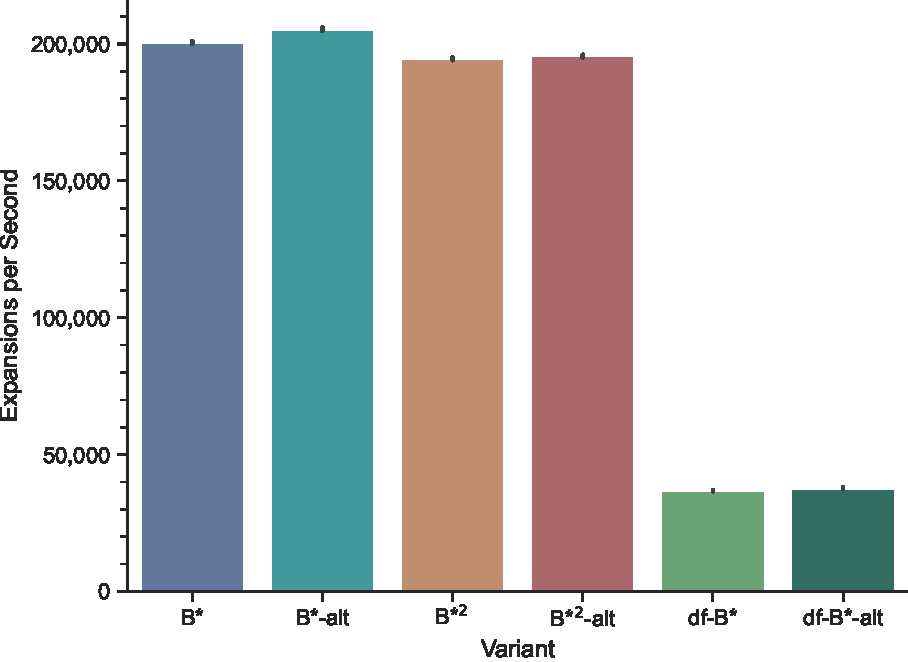
\includegraphics[scale=0.7]
	{figures/graphs/colour/fig1ExpansionsPerSecondAllTrees.pdf}
	\fi
	\caption{This figure shows the average number of nodes expanded per second of runtime (average of ratios), grouped by algorithm variant. Shown are all runs on 13\thsep936 trees for which no runtime was less than 0.0005 seconds.
    Also shown are 95\% confidence intervals.}
	\label{fig:Exp1ExpansionsPerSecondAllTrees}
\end{figure}
\FloatBarrier

\paragraph{Memory Usage.} We compare the memory usage of different algorithm variants. Averaged over all 1\thsep192\thsep320 runs, as shown in Figure \ref{fig:Exp1NodesPerAlgAllRuns}, we found that \textbf{B*}
$\left(\approx\text{181\thsep100}\pm4400\right)$
and \textbf{B*-alt}
$\left(\approx\text{184\thsep400}\pm4500\right)$
stored the most nodes in memory. Whereas \textbf{B*}$^2$ 
$\left(\approx\text{37\thsep830}\pm990\right)$
and \textbf{B*}$^2$\textbf{-alt}
$\left(\approx\text{38\thsep250}\pm1000\right)$
stored significantly fewer nodes in memory. Additionally, we recorded the maximum number of nodes on the execution stack for \textbf{df-B*}
$\left(\approx4130\pm83\right)$
and \textbf{df-B*-alt}
$\left(\approx3910\pm80\right)$.
However, the memory usage of \textbf{df-B*} and \textbf{df-B*-alt} is effectively constant, as both variants always keep a transposition table in memory, with a size of $2^{20}=\text{1\thsep048\thsep576}$ nodes, as described in Subsection \ref{subsec:Exp1:Algorithms}.
Figure \ref{fig:Exp1NodesPerExpansionsSolvedByAny} shows the relationship between expansions and nodes stored in memory, grouped by B* (\textbf{B*} and \textbf{B*-alt}), ${\text{B*}}^2$ (\textbf{B*}$^2$ and \textbf{B*}$^2$\textbf{-alt}), and df-B* (\textbf{df-B*} and \textbf{df-B*-alt}). The algorithm variants have been grouped by their core technique because there was no visible difference between the grouped variants. The graph shows how the three B* techniques handle memory differently. Among all solved runs, we find that B* stored at most 1\thsep048\thsep526 nodes in memory, whereas ${\text{B*}}^2$ stored at most 281\thsep270 nodes in memory, and df-B* stored at most 10\thsep955 nodes in the stack. Zooming in on B*, we find that the rate of nodes stored per expansion is correlated with the branching factor ($r\approx0.87$), which is an expected result.
%
% NODE GRAPHS:
%
\begin{figure}[htbp]
	\centering
	\ifMonochrome
	
\includegraphics[scale=0.7]
	{figures/graphs/monochrome/fig1NodesPerExpansionsSolvedByAny.pdf}
	\else
	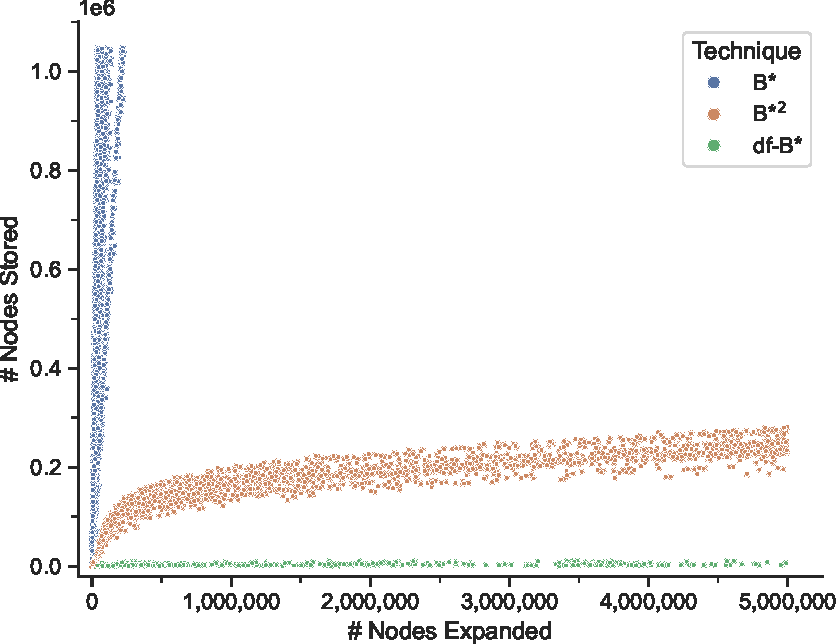
\includegraphics[scale=0.7]
	{figures/graphs/colour/fig1NodesPerExpansionsSolvedByAny.pdf}
	\fi
	\caption{This figure shows the maximum number of nodes stored in memory, during a run, plotted against the number of nodes expanded, grouped by search technique. Only the 1\thsep005\thsep723 solved runs are shown. Values for df-B* are measured as the maximum number of nodes stored in the stack during the search, whereas the majority of df-B* memory usage is constant and determined by the size of the transposition table ($2^{20}=\text{1\thsep048\thsep576}$).}
	\label{fig:Exp1NodesPerExpansionsSolvedByAny}
\end{figure}
%
\begin{figure}[htbp]
	\centering
	\ifMonochrome
	
\includegraphics[scale=0.6125]
	{figures/graphs/monochrome/fig1NodesPerAlgAllRuns.pdf}
	\else
	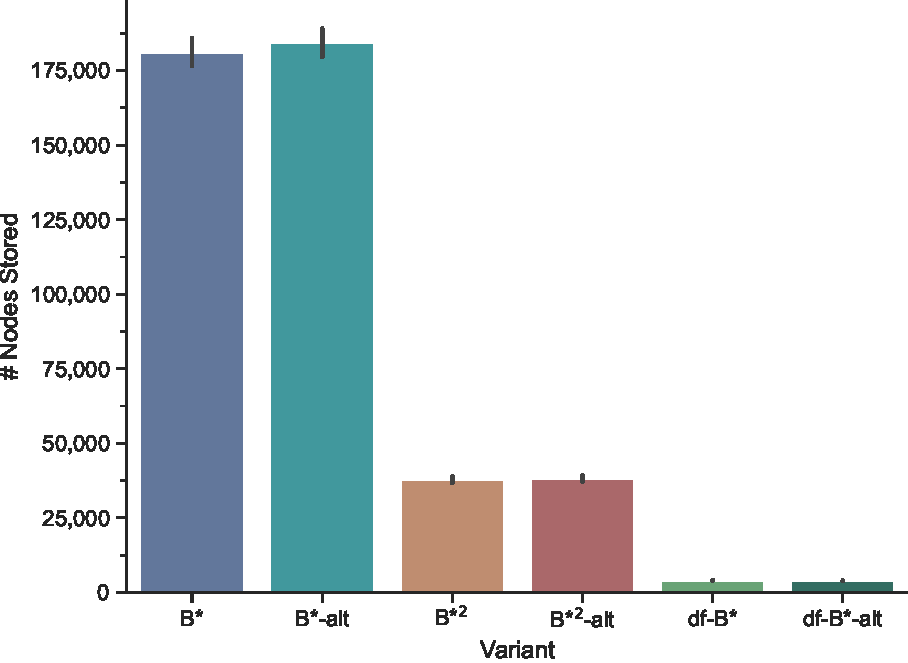
\includegraphics[scale=0.6125]
	{figures/graphs/colour/fig1NodesPerAlgAllRuns.pdf}
	\fi
	\caption{This figure shows the average number of nodes maximally stored in memory by each algorithm variant. All 1\thsep192\thsep320 runs are included. Values for df-B* are measured as the maximum number of nodes stored in the stack during the search.}
	\label{fig:Exp1NodesPerAlgAllRuns}
\end{figure}
%
\paragraph{Extra.} In addition to these results, Table \ref{tab:RelativePerformance} in the Appendix shows the relative performance of the six algorithm variants in terms of expansions, nodes stored, and run duration.
\FloatBarrier
\subsection{Experiment 2}
\label{subsec:ResultsExp2}
The results from Experiment\ 2 include the recorded metrics of 720\thsep000 runs on 12\thsep000 trees, as described in Subsection \ref{subsec:Exp2}. With these results, we explore the memory usage of ${\text{B*}}^2$ in more detail.
For this experiment, we look at one key metric: the number of nodes stored in memory. We also record, for each run, whether it was `solved' or `unsolved', based on separation at the root node. We analyse the results mostly on a per-tree basis. For each tree, the results include 10 runs of \textbf{B*}, 25 runs of \textbf{B*}$^2$, and 25 runs of \textbf{B*}$^2$\textbf{-max}. 
In this subsection, unless stated otherwise, the number of nodes stored by an algorithm variant on a tree refers to the minimum among all runs on that tree, excluding unsolved runs. For an initial comparison, we look at the set of 8733 trees which were solved at least once by all variants. Here, we find that \textbf{B*}$^2$
$\left(\approx54\text{\thsep}800\pm1600\right)$
stored significantly more nodes in memory, on average, than \textbf{B*}$^2$\textbf{-max}
$\left(\approx3720\pm100\right)$. Whereas \textbf{B*}
$\left(\approx617\text{\thsep}000\pm27\text{\thsep}000\right)$ stored the most nodes in memory on average. The following results go into further detail.

Figure \ref{fig:Exp2MemoryFootprintBoth} shows the main result of this experiment: the memory footprint of ${\text{B*}}^2$. We directly compare the memory usage of \textbf{B*} to the memory usage of \textbf{B*}$^2$ and \textbf{B*}$^2$\textbf{-max}, where memory usage is represented in terms of the minimum number of nodes needed to solve a tree. The one-on-one data, including points for each of the 12\thsep000 trees, is shown in Figure \ref{fig:Exp2MemoryFootprintBothRaw}. Here, some variance in algorithm performance on various trees is visible. We can see that \textbf{B*}$^2$ has a sub-linear memory footprint relative to \textbf{B*}'s memory usage. This relationship is shown more clearly in Figure \ref{fig:Exp2MemoryFootprintBothGroups5}. Each point is the average result of 5 trees, adjacent in terms of \textbf{B*}'s memory usage on those trees. We can also fit a line to this pattern. Fitting a $y=a\sqrt{x}$ line, where $y$ is \textbf{B*}$^2$'s memory usage and $x$ is \textbf{B*}'s memory usage, results in a good fit overall ($a=114\to R^2\approx0.92$), but overshoots greatly where $x > \text{500\thsep000}$ ($a=116\to R^2\approx0.58$). Figure \ref{fig:Exp2MemoryFootprintMaxGroups2} looks at the same result, but zoomed in on \textbf{B*}$^2$\textbf{-max}. However, fitting the same line to this plot gives a more consistent result. The line $y=a\sqrt{x}$ fits well overall ($a=7.6\to R^2\approx 0.92$), and still fits for $x > 500\text{\thsep}000$ ($a=7.6\to R^2\approx 0.76$). This line $y=7.6\sqrt{x}$ is displayed on top of the results from Experiment\ 2 in Figure \ref{fig:Exp2MemoryFootprintMaxGroups2}, which shows that the data visually matches it.
%
\begin{figure}[htbp]
\centering
\begin{subfigure}{.5\textwidth}
	\centering
	\ifMonochrome
	
\includegraphics[width=\linewidth]
	{figures/graphs/monochrome/fig2MemoryFootprintBothRaw.pdf}
	\else
	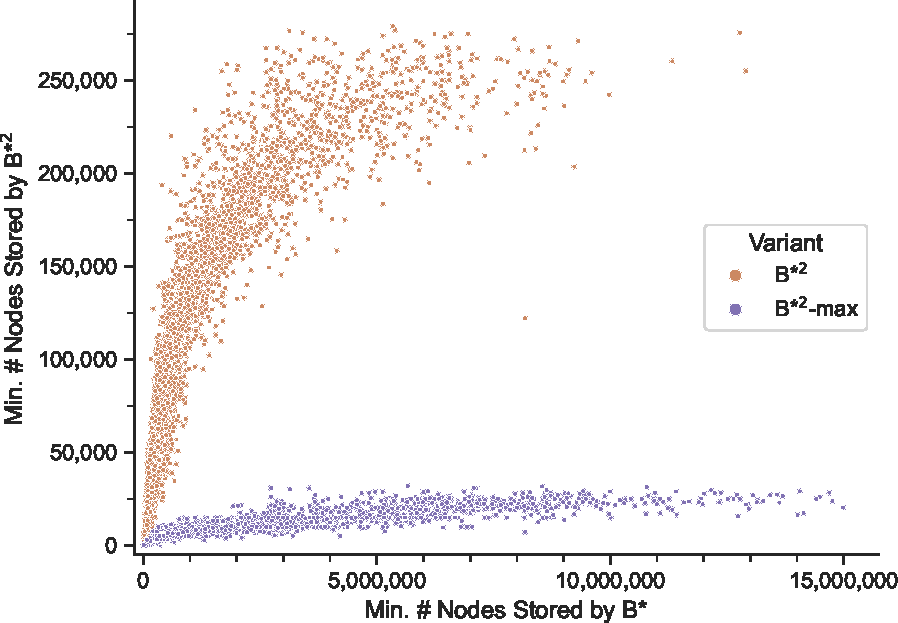
\includegraphics[width=\linewidth]
    {figures/graphs/colour/fig2MemoryFootprintBothRaw.pdf}
	\fi
	\caption{Ungrouped: each dot corresponds to one tree}
	\label{fig:Exp2MemoryFootprintBothRaw}
\end{subfigure}%
\begin{subfigure}{.5\textwidth}
\centering
	\ifMonochrome
	
\includegraphics[width=\linewidth]
	{figures/graphs/monochrome/fig2MemoryFootprintBothGroups5.pdf}
	\else
	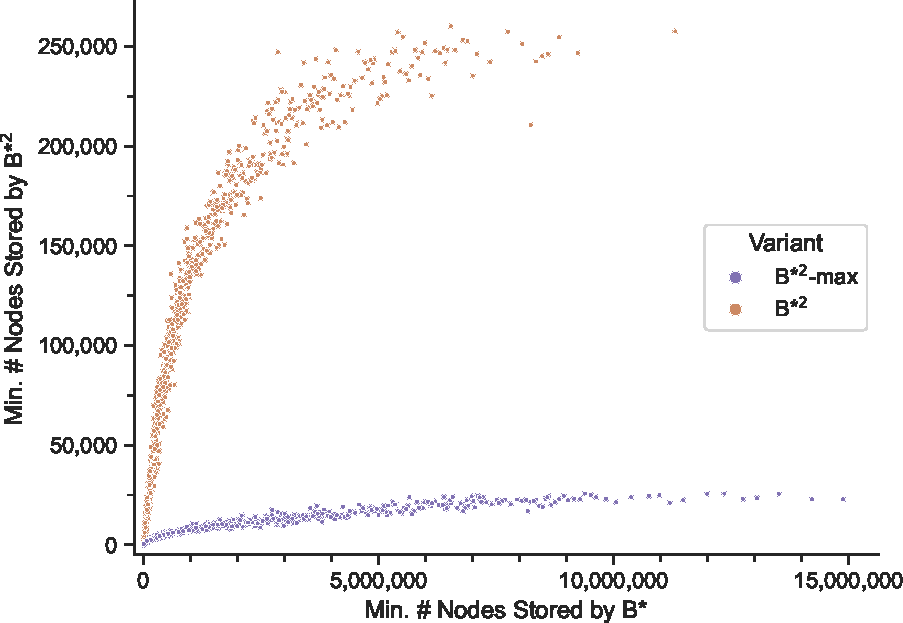
\includegraphics[width=\linewidth]
	{figures/graphs/colour/fig2MemoryFootprintBothGroups5.pdf}
	\fi
	\subcaption{Grouped: each dot corresponds to 5 trees}
	\label{fig:Exp2MemoryFootprintBothGroups5}
\end{subfigure}
\caption{This figure shows the memory footprint of \textbf{B*}$^2$ and \textbf{B*}$^2$\textbf{-max} relative to \textbf{B*} on the set of 9087 trees solved by \textbf{B*} and at least one other variant. On the \textbf{left (a)}, the X-axis shows the minimum number of nodes stored in memory by \textbf{B*} out of 10 runs performed on the same tree. The Y-axis shows the minimum number of nodes stored in memory by \textbf{B*}$^2$ or \textbf{B*}$^2$\textbf{-max} out of 25 runs performed on the same tree, only including solved runs. The \textbf{right (b)} figure shows the averages of 5 adjacent trees, ordered by X-axis value, for the plotted X and Y values in Figure (a). Thus, each dot corresponds to 50 runs of \textbf{B*} and 125 runs of \textbf{B*}$^2$ or \textbf{B*}$^2$\textbf{-max}.}
\label{fig:Exp2MemoryFootprintBoth}
\end{figure}
%%%%%%%%%%%%%%%%%%%%%%%%
% \begin{figure}[h!]
% 	\centering
% 	\ifMonochrome
% 	\includegraphics[scale=0.7]
% 	{figures/graphs/monochrome/fig2MemoryFootprintBothRaw.pdf}
% 	\else
% 	\includegraphics[scale=0.7]
% 	{figures/graphs/colour/fig2MemoryFootprintBothRaw.pdf}
% 	\fi
% 	\caption{MemoryFootprintBothRaw}
% 	\label{fig:Exp2MemoryFootprintBothRaw}
% \end{figure}
%
% \begin{figure}[htbp]
% 	\centering
% 	\ifMonochrome
% 	\includegraphics[scale=0.7]
% 	{figures/graphs/monochrome/fig2MemoryFootprintBothGroups5.pdf}
% 	\else
% 	\includegraphics[scale=0.7]
% 	{figures/graphs/colour/fig2MemoryFootprintBothGroups5.pdf}
% 	\fi
% 	\caption{MemoryFootprintBothGroups5}
% 	\label{fig:Exp2MemoryFootprintBothGroups5}
% \end{figure}
%%%%%%%%%%%%%%%%%%%%%%%%%%%%%%%%%%%%%%%%%%%%
%
% \begin{figure}[htbp]
% 	\centering
% 	\ifMonochrome
% 	\includegraphics[scale=0.7]
% 	{figures/graphs/monochrome/fig2MemoryFootprintMaxRaw.pdf}
% 	\else
% 	\includegraphics[scale=0.7]
% 	{figures/graphs/colour/fig2MemoryFootprintMaxRaw.pdf}
% 	\fi
% 	\caption{MemoryFootprintMaxRaw}
% 	\label{fig:Exp2MemoryFootprintMaxRaw}
% \end{figure}
%
\begin{figure}[htbp]
	\centering
	\ifMonochrome
	
\includegraphics[scale=0.7]
	{figures/graphs/monochrome/fig2MemoryFootprintMaxGroups2.pdf}
	\else
	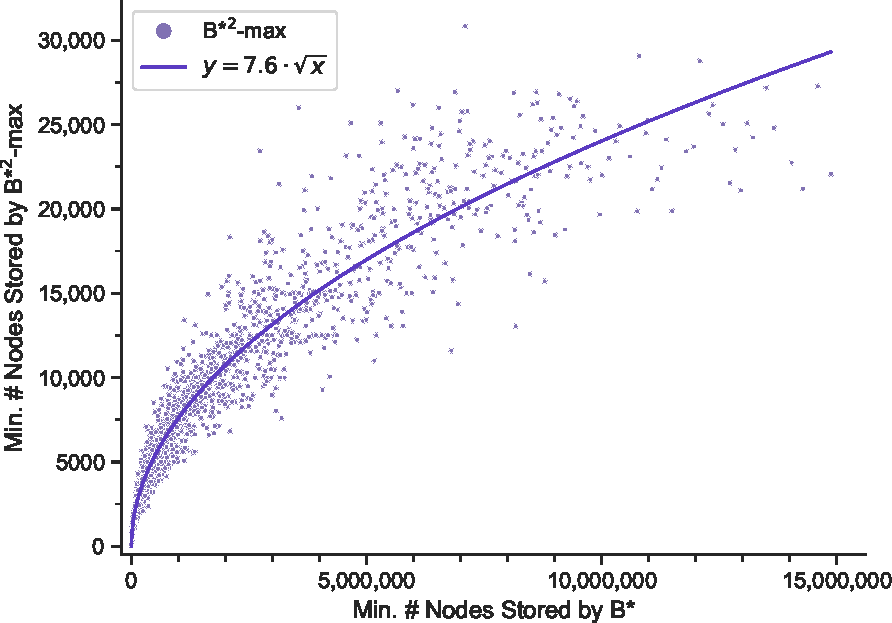
\includegraphics[scale=0.7]
	{figures/graphs/colour/fig2MemoryFootprintMaxGroups2.pdf}
	\fi
	\caption{This figure shows the memory footprint of \textbf{B*}$^2$\textbf{-max} relative to \textbf{B*} on the set of 9080 trees solved by both variants. The X-axis shows the average over 2 trees of the minimum number of nodes stored in memory by \textbf{B*} out of 10 runs performed on the same tree. The Y-axis shows the average over 2 trees of the minimum number of nodes stored in memory by \textbf{B*}$^2$\textbf{-max} out of 25 runs performed on the same tree, only including solved runs. Thus, each dot corresponds to 20 runs of \textbf{B*} and 50 runs of \textbf{B*}$^2$\textbf{-max}. Additionally, a fit-line for the function $y=a\cdot\sqrt{x}$, with $a=7.6$ is plotted. The coefficient of determination of the fitted line is $R^2\approx 0.92$}
	\label{fig:Exp2MemoryFootprintMaxGroups2}
\end{figure}
%
\paragraph{Extrapolation.}
Observe the line fit for \textbf{B*}$^2$\textbf{-max} in Figure \ref{fig:Exp2MemoryFootprintMaxGroups2}: $y=7.6\cdot\sqrt{x}$. It describes the amount of memory used by \textbf{B*}$^2$\textbf{-max} relative to \textbf{B*}. But what does this relationship mean for the size of trees \textbf{B*}$^2$\textbf{-max} can solve? Let $N$ be the maximum size tree \textbf{B*} can solve, in terms of number of nodes in memory. Then, inverting this equation, and assuming it can be extrapolated, we get that \textbf{B*}$2$\textbf{-max} may be able to solve trees with up to $\approx0.017\cdot N^2$ number of nodes as searched by \textbf{B*}. This is a very substantial increase, given the order of $N^2$. However, this result may be inconclusive as the fit excludes 207 trees unsolved by \textbf{B*}$^2$\textbf{-max} that were solved by \textbf{B*}. The memory usage of \textbf{B*}$^2$\textbf{-max} for these trees is unknown, as they exceeded the expansion limit of the search.
%
% \begin{figure}[htbp]
% 	\centering
% 	\ifMonochrome
% 	\includegraphics[scale=0.7]
% 	{figures/graphs/monochrome/fig2MemoryFootprintMaxGroups5.pdf}
% 	\else
% 	\includegraphics[scale=0.7]
% 	{figures/graphs/colour/fig2MemoryFootprintMaxGroups5.pdf}
% 	\fi
% 	\caption{MemoryFootprintMaxGroups5}
% 	\label{fig:Exp2MemoryFootprintMaxGroups5}
% \end{figure}
%
% \begin{figure}[htbp]
% 	\centering
% 	\ifMonochrome
% 	\includegraphics[scale=0.7]
% 	{figures/graphs/monochrome/fig2NodesExpandedByNodeLimitAllSolved.pdf}
% 	\else
% 	\includegraphics[scale=0.7]
% 	{figures/graphs/colour/fig2NodesExpandedByNodeLimitAllSolved.pdf}
% 	\fi
% 	\caption{NodesExpandedByNodeLimitAllSolved}
% 	\label{fig:Exp2NodesExpandedByNodeLimitAllSolved}
% \end{figure}
%
\FloatBarrier
\paragraph{Efficiency of \texorpdfstring{${\text{B*}}^2$}{B*²}-max}
Finally, there are some additional results comparing \textbf{B*}$^2$ to \textbf{B*}$^2$\textbf{-max}. Figure \ref{fig:Exp2TreesSolvedByNodeLimit} shows which percentage of all 12\thsep000 trees each ${\text{B*}}^2$ variant solved, where runs are grouped by their node limit. The figure shows that \textbf{B*}$^2$\textbf{-max} solves few to none new trees when the node limit is increased beyond 25\thsep000, whereas \textbf{B*}$^2$ reaches this point for node limits beyond 275\thsep000. Beyond this point, the main limitation for both variants is the expansion limit rather than the node limit, which is 10\thsep000\thsep000 nodes for Experiment 2. It is also shown that \textbf{B*}$^2$ solved fewer trees (8741) compared to \textbf{B*}$^2$\textbf{-max} (9080). Figure \ref{fig:Exp2SolvedTreesSurvivalByTreeSize} shows the difference in the number of trees solved by \textbf{B*}$^2$ and \textbf{B*}$^2$\textbf{-max} compared to the memory footprint of \textbf{B*} on these trees. This is a measure of algorithm efficiency rather than memory usage, because both \textbf{B*}$^2$ and \textbf{B*}$^2$\textbf{-max} are primarily restricted by the expansion limit, as shown in Figure \ref{fig:Exp2TreesSolvedByNodeLimit}. Here, \textbf{B*}$^2$\textbf{-max} is shown to solve larger trees more effectively than \textbf{B*}$^2$. Additionally, on solved trees for which \textbf{B*} stored $\ge10\text{\thsep}000\text{\thsep}000$ nodes, 3 were solved by \textbf{B*}$^2$ and 61 were solved by \textbf{B*}$^2$\textbf{-max}. Out of the trees unsolved by \textbf{B*}, 1 was solved by \textbf{B*}$^2$ and 32 were solved by \textbf{B*}$^2$\textbf{-max}, with at most $\sim$32\thsep000 nodes in memory, compared to $\sim$250\thsep000 for \textbf{B*}$^2$.
\begin{figure}[htbp]
	\centering
	\ifMonochrome
	
\includegraphics[scale=0.7]
	{figures/graphs/monochrome/fig2TreesSolvedByNodeLimit.pdf}
	\else
	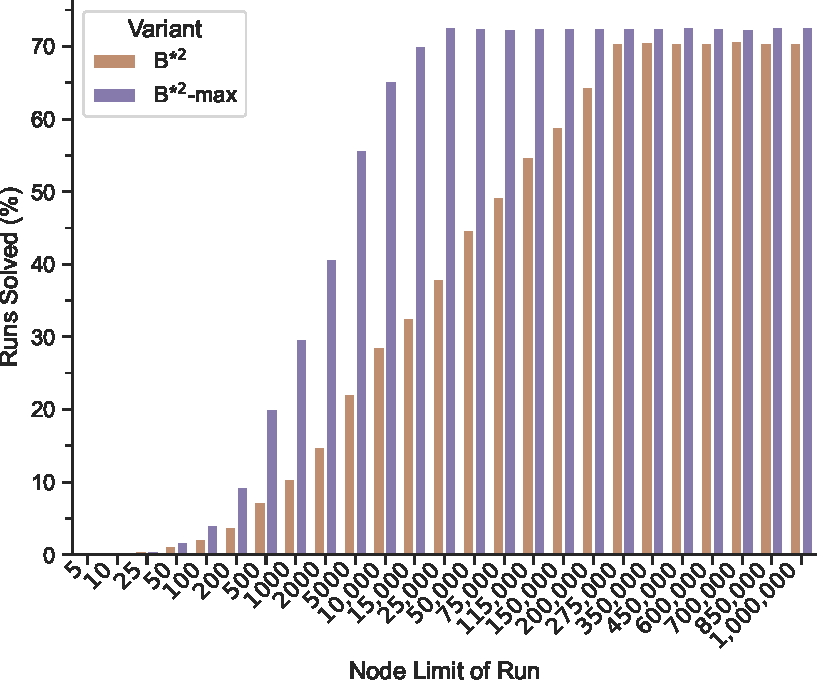
\includegraphics[scale=0.7]
	{figures/graphs/colour/fig2TreesSolvedByNodeLimit.pdf}
	\fi
	\caption{This figure shows the percentage of trees, out of the 12\thsep000 included in Experiment 2, solved by \textbf{B*}$^2$ or \textbf{B*}$^2$\textbf{-max} for each of the 25 different node limits imposed on the search. The X-axis of this figure is a list of all node limits and does not follow a linear scale.}
	\label{fig:Exp2TreesSolvedByNodeLimit}
\end{figure}
%
\begin{figure}[htbp]
	\centering
	\ifMonochrome
	
\includegraphics[scale=0.7]
	{figures/graphs/monochrome/fig2SolvedTreesSurvivalByTreeSize.pdf}
	\else
	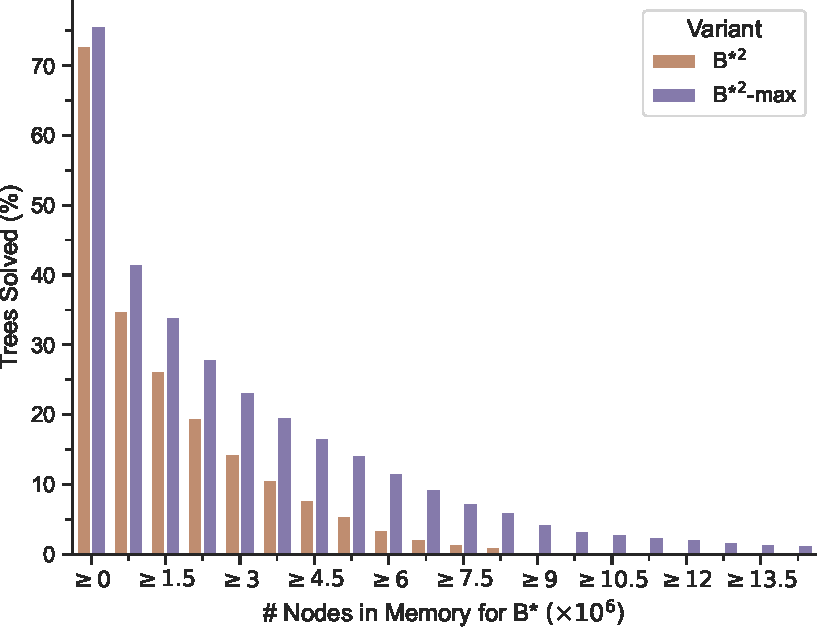
\includegraphics[scale=0.7]
	{figures/graphs/colour/fig2SolvedTreesSurvivalByTreeSize.pdf}
	\fi
    \caption{This figure shows, for each group of trees, the percentage that was solved by \textbf{B*}$^2$ or by \textbf{B*}$^2$\textbf{-max}. Each bar shows the group of trees, out of a total of 12\thsep000, for which \textbf{B*} required at least the specified number of nodes in memory to solve. The leftmost bar includes all 12\thsep000 trees from Experiment 2, whereas the rightmost bar includes only those trees for which \textbf{B*} stored $\ge$ 14\thsep250\thsep000 nodes in memory.}
	\label{fig:Exp2SolvedTreesSurvivalByTreeSize}
\end{figure}

\chapter{Conclusions and Future Research}
\label{cht:Conclusions}
This chapter concludes the thesis. The research questions posed in the introduction are addressed in Section \ref{sec:Conclusions:RQs}, and the problem statement is reassessed in Section \ref{sec:Conclusions:ProblemStatement}. Finally, we propose ideas for future research in Section \ref{sec:FutureResearch}.

\section{Research Questions}
\label{sec:Conclusions:RQs}
This section assesses the three research questions posed in Section \ref{sec:problemStatementAndRQs} of the introduction. 

\paragraph{1.} \textit{How can B* be adapted to multi-level (${\text{B*}}^{\text{\hspace{1pt}}\textit{2}}$) or depth-first (df-B*) search?}\\

\vspace{-1ex}
\noindent This question was posed to guide the design of the novel techniques introduced in this thesis.
We draw inspiration from existing techniques, but there are several defining differences.
The ${\text{B*}}^2$ and df-B* techniques differ from the techniques they are based on, ${\text{PN}}^2$ \cite{Breuker1998} and df-PN \cite{Nagai2002}, by the adaptations made to apply their concepts to the domain of B*:
\textbf{(a)} ${\text{B*}}^2$ differs from ${\text{PN}}^2$ by the nuance of strategy selection at each level of the search, and by the additional stop conditions for the second-level search. These adaptations are a natural result of adapting B* to multi-level search.
\textbf{(b)} df-B* differs from df-PN by the separation between the root-level search and search on internal nodes. This is a natural result of strategy selection in B*. The separation between $\epsilon$ and $\sigma$ is also a natural result, as inspired by \citeA{PawlewiczLew2007}, because df-B* may benefit from more frequent back-ups to the root, through reconsideration of the search strategy. Finally, df-B* reads values of solved nodes from the transposition table to prune them early, similar to df-PN. However, df-B* may also prune nodes that were not solved before, but have become irrelevant due to updates to other nodes. This is a natural result of node pruning in B* that is not present in Proof-Number Search (PNS) or df-PN.

\paragraph{2.} \textit{How do ${\text{B*}}^{\text{\hspace{1pt}}\textit{2}}$ and df-B* affect the memory usage of search compared to B*?}\\

\vspace{-1ex}
\noindent The main goal of developing ${\text{B*}}^2$ and df-B* was to reduce the memory usage of B*. This research question aims to quantify the extent to which these techniques succeed in that goal. We first describe the resolution of this research question for ${\text{B*}}^2$, and then for df-B*.\\

\noindent \textbf{B*}$^2$ is shown, in Figure \ref{fig:Exp2MemoryFootprintBoth}, to require significantly less memory than B* to solve the same trees. This is highlighted in Subsection \ref{subsec:ResultsExp1} as well as in Subsection \ref{subsec:ResultsExp2}. Table \ref{tab:RelativePerformance} shows that, on the trees examined in Experiment 1, ${\text{B*}}^2$ required between 15\% and 17\% of the number of nodes in memory as B* to solve the same sets of trees. For Experiment 2, as described in Subsection \ref{subsec:ResultsExp2}, we found that, on the set of 8733 trees solved by both, B* stored on average 617\thsep000 nodes and ${\text{B*}}^2$ on average 54\thsep800. That is a ratio of 9\% on that specific set of trees. However, these averages on specific sets of trees are only indicative results. A more conclusive result is shown in Figure \ref{fig:Exp2MemoryFootprintBoth} and Figure \ref{fig:Exp2MemoryFootprintMaxGroups2}. The latter of which approximately quantifies $y=7.6\sqrt{x}$ ($R^2\approx0.92$) as the relationship describing the relative memory usage of ${\text{B*}}^2$ ($y$) to B* ($x$). The inverse of this suggests that ${\text{B*}}^2$, given the same memory limitations as B*, may be able to solve trees of sizes up to $\approx0.017\cdot N^2$, where $N$ is the memory usage of the maximum size trees solved by B*.
This result assumes the maximum second-level tree-size limit is applied for ${\text{B*}}^2$ (see Subsection \ref{subsec:Level2SizeLimit}).
These results show that ${\text{B*}}^2$ can solve larger trees than B*, but still has an upper limit of trees that can be solved based on the available memory.
This aligns with existing research on multi-level search techniques. First, \citeA{BaumSmith1997} hypothesised a square-root relationship in memory usage of a two-stage Bayesian Search, which matches our result. Second, \citeA{Breuker1998} similarly found significantly reduced memory usage of ${\text{PN}}^2$ compared to PNS, which we also observe for ${\text{B*}}^2$.\\

\noindent \textbf{df-B*} uses a transposition table and execution stack for memory. The transposition table utilises constant memory, whereas the execution stack stores at most $b\cdot d$ nodes, where $b$ is the branching factor of the tree and $d$ is the maximum depth of the search. The memory usage of the stack is included in our results, as shown in Figure \ref{fig:Exp1NodesPerExpansionsSolvedByAny} and Figure \ref{fig:Exp1NodesPerAlgAllRuns}. Subsection \ref{subsec:ResultsExp1} describes that df-B* stored at most 10\thsep955 nodes in its execution stack compared to over a million nodes stored in memory for B*, on solved trees of Experiment 1. For the purpose of comparing the memory usage of df-B* to B*, df-B* only uses constant memory, as the memory usage of df-B* is in the order of $b\cdot d$ rather than the $b^d$ for B*.
This result is as expected; df-B* can search very large trees with effectively no limit on the size of trees that can be solved, if given enough time.

\paragraph{3.} \textit{How do ${\text{B*}}^{\text{\hspace{1pt}}\textit{2}}$ and df-B* compare to B* in terms of computational efficiency?}\\

\vspace{-1ex}
\noindent We compare the computational efficiency of ${\text{B*}}^2$ and df-B* to B* to understand the cost of reduced memory usage. As to achieve this reduced memory usage, both techniques actively discard a large portion intermediate search results. This comes at a computational cost, which we mostly measure in the number of expansions performed during the search. We first describe the results for computational efficiency of ${\text{B*}}^2$, and then of df-B*.\\

\noindent \textbf{B*}$^2$ surprisingly seems not to always give up on computational efficiency in exchange for reduced memory usage. Subsection \ref{subsec:ResultsExp1} describes how, when the expansion limit was reduced to 1\thsep000\thsep000, which is less than the applied node limit, ${\text{B*}}^2$ still solved $0.06\%$ more trees than B*. This shows that ${\text{B*}}^2$ may sometimes solve the same trees more efficiently than B* does. However, Subsection \ref{subsec:ResultsExp1} and Figure \ref{fig:Exp1ExpansionsPerAlgSolvedByAll} show that ${\text{B*}}^2$ performed on average 56\% more expansions than B* on the set of 15\thsep131 universally solved trees from Experiment 1.
Table \ref{tab:RelativePerformance} also shows that ${\text{B*}^2}$ expanded between 2.6 and 3 times as many nodes as B* on the same sets of over 22\thsep000 trees. We conclude that the latter is likely a more realistic result, as the set of universally solved trees is biased by the reduced set of trees solved by df-B*.

Additionally, Figure \ref{fig:Exp1ExpansionsPerSecondAllTrees} shows that ${\text{B*}}^2$ has a comparable rate of expansion to B*, which corresponds to a similar computational overhead for the two techniques. As a result, the runtime of ${\text{B*}}^2$ scales predictably with its increased number of expansions compared to B*.

Experiment\ 2 shows an additional result on the computational efficiency of ${\text{B*}}^2$. Figure \ref{fig:Exp2SolvedTreesSurvivalByTreeSize} shows that, compared to the ${\text{B*}}^2$ variant shown in Experiment 1, ${\text{B*}}^2$ with the maximum tree-size limit more efficiently solves larger trees, despite neither variant ever terminating due to the upper node limit of 1\thsep000\thsep000 nodes. This indicates that the computational efficiency of ${\text{B*}}^2$ might be improved by modifying the tree-size limits of the second-level search.\\

\noindent \textbf{df-B*} is found to have a significantly reduced computational efficiency compared to B*, as seen in Figure \ref{fig:Exp1SolvedPerAlgAllRuns}, Figure \ref{fig:Exp1ExpansionsPerAlgSolvedByAll}, and Figure \ref{fig:Exp1ExpansionsPerSecondAllTrees}. Table \ref{tab:RelativePerformance} shows that df-B* expands on average between 22 and 23 times as many nodes as B* on the same sets of trees.
However, the results from Figure \ref{fig:Exp1ExpansionsPerSecondAllTrees} show that df-B* also has significantly increased computational overhead compared to B* and ${\text{B*}}^2$. Similarly, \citeA{Winands2004} found, for the implementation of the PNS variant PDS-PN, that the depth-first PDS search \cite{Nagai1999} had a significant amount of computational overhead compared to PNS and ${\text{PN}}^2$.
The computational overhead may therefore be a more systemic problem with depth-first game-tree solvers, although this would require additional research to confirm.
Nevertheless, the computational efficiency of df-B* may be increased with further research into the technique. Our implementation of df-B* is not optimal. Compared to B* and ${\text{B*}}^2$, which have been modified to improve their performance on this domain, df-B* is implemented in this thesis as its minimum viable version. As such, there is likely room for improvement, at least in the number of expansions needed to solve the same trees.

\section{Problem Statement}
\label{sec:Conclusions:ProblemStatement}
We reassess the problem statement of this thesis, which was formulated as follows:
\\[1\baselineskip]
\textit{How can B* be extended to search on much larger problems?}
\\[1\baselineskip]
By applying inspirations from the memory-efficient PNS variants ${\text{PN}}^2$ and df-PN, B* can be extended to solve larger problems. Results on problems of up to 15 million nodes in size show that ${\text{B*}}^2$ may solve problems of up to 0.017 times the square of the size of problems as solved by B*. The memory usage of ${\text{B*}}^2$ is in the order of a square-root of the memory usage by B*. To search even larger problems, multiple levels of B* can be chained together for ${\text{B*}}^k$, which is expected to use memory in the order of a $k$-root of the memory used by B*. Additionally, the depth-first B* variant df-B* can effectively search any size trees, with near constant memory usage, if given enough time. Overall, we conclude that ${\text{B*}}^2$ is a good alternative to B* when searching relatively large problems with limited memory, whereas df-B* is a good alternative to B* when searching very large problems of undetermined size.
% \section{Limitations}
% \label{sec:Limitations}
\section{Future Research}
\label{sec:FutureResearch}
This section concludes this thesis by suggesting directions for future research.

\textbf{First}, we suggest that future research explore more domains to which B* can be applied. 
We find that B* does not have to be limited by memory, as ${\text{B*}}^2$ works efficiently while reducing its memory usage, and df-B* can solve problems regardless of their size. This may allow for B* to be applied to domains that it was not applicable to before. B* does not need to be restricted to game-tree search domains. It may solve any problem which can be represented as a tree with lower and upper bounds on some value to be optimised. Therefore, ${\text{B*}}^2$ and df-B* may expand the possibilities of B* by reducing or removing its memory limitation. Additionally, the domain we apply in this thesis is different from many other domains in that its underlying structure does not contain any transpositions (see Section \ref{sec:AGTmodel}). Whereas df-B* is expected to solve trees with transpositions more efficiently, as results from the use of a transposition table (see Subsection \ref{subsec:dfBstarChallenges:Transpositions}). As a result, other domains may show better performance of df-B*.

\textbf{Second}, future research could explore a novel idea to improve B* and its variants: (dis)proof numbers for value ranges. An interesting finding from our preliminary experiments was that ${\text{B*}}^2$ seemed to perform much better, in all aspects, than B* on certain large trees. To combat this, we implemented two adjustments for B*, which are described in Section \ref{sec:BstarAdjustments}: a maximum to the number of rootless updates, and a random chance to select an alternative node at internal node selection. The effectiveness of the latter modification and the randomness of its function suggest that there may be more room for improvement in internal node selection, which is not a new idea \cite{Palay1983, Berliner1996}. This problem has been addressed with probabilistic B*, but this approach lacks a metric for measuring the amount of work needed to progress on a sub-tree. Here we can take inspiration from PNS once again, and introduce the idea of (dis)proof numbers to B*. A (dis)proof number in B* can represent the minimum number of expansions required to (dis)prove the value of a node lies above a certain threshold. The main problem with this approach is that a range of (dis)proof numbers may be needed for each of multiple thresholds. However, as of the time of writing, this is a mostly unexplored concept with the potential to improve B*, ${\text{B*}}^2$, df-B*, and even PB* \cite{Palay1983}.

\textbf{Third}, future research could evaluate several enhancements to ${\text{B*}}^2$. This includes the stop conditions for shallow and deep irrelevance, and the four bounds preservation approaches mentioned in Subsection \ref{subsec:BstarSquaredAlgorithm:BoundsPreservation}. Lazy evaluation may also be applied to ${\text{B*}}^2$, which we have not implemented in this thesis. Exploring the promise of these enhancements may give a fuller picture of the potential of ${\text{B*}}^2$ and multi-level search in general.

\textbf{Finally}, we suggest future research explore the potential of df-B* further.
Our findings show promise for df-B*, but also challenges. Our implementation of df-B*, as described in this thesis, is far from optimal. We expect that the computational efficiency of df-B* can be greatly increased by implementing a better internal node selection and by including a metric for required work on sub-trees. df-B* could also be improved with a more informed replacement scheme for the transposition table. Additionally, df-B* may have more potential on domains with many transpositions, as mentioned in Section \ref{subsec:dfBstarChallenges:Transpositions}.

%%%% Bibliography %%%%
% Apply a small adjustment to the margins and the line-spacing
%  to allow everything to fit in 2 pages
% \begingroup
% \linespread{0.98}\selectfont
\begin{adjustwidth}{0pt}{-4pt}
\bibliographystyle{apacite-list-all-authors}
\bibliography{bibliography.bib}
\end{adjustwidth}
% \endgroup

\newpage
\begin{appendix}
    \chapter{Additional Tables}
\begin{table}[h]
    \centering
\begin{tabular}{lll|c}
Branching Factor $b$ & Distribution Factor $k$ & Growth Factor $g$ & Allocated Seeds $S_0$ \\ \hline
\multirow[c]{8}{*}{{\cellcolor[HTML]{F7FBFF}}} 5 & \multirow[c]{4}{*}{{\cellcolor[HTML]{F7FBFF}}} 5 & {\cellcolor[HTML]{F7FBFF}} 1.2 & 0 \\
{\cellcolor[HTML]{F7FBFF}}  & {\cellcolor[HTML]{F7FBFF}}  & {\cellcolor[HTML]{CCDFF1}} 1.3 & 1 \\
{\cellcolor[HTML]{F7FBFF}}  & {\cellcolor[HTML]{F7FBFF}}  & {\cellcolor[HTML]{82BBDB}} 1.4 & 2 \\
{\cellcolor[HTML]{F7FBFF}}  & {\cellcolor[HTML]{F7FBFF}}  & {\cellcolor[HTML]{58a9d6}} 1.5 & 3 \\
{\cellcolor[HTML]{F7FBFF}}  & \multirow[c]{4}{*}{{\cellcolor[HTML]{6AAED6}}} 6 & {\cellcolor[HTML]{F7FBFF}} 1.2 & 4 \\
{\cellcolor[HTML]{F7FBFF}}  & {\cellcolor[HTML]{6AAED6}}  & {\cellcolor[HTML]{CCDFF1}} 1.3 & 5 \\
{\cellcolor[HTML]{F7FBFF}}  & {\cellcolor[HTML]{6AAED6}}  & {\cellcolor[HTML]{82BBDB}} 1.4 & 6 \\
{\cellcolor[HTML]{F7FBFF}}  & {\cellcolor[HTML]{6AAED6}}  & {\cellcolor[HTML]{58a9d6}} 1.5 & 7 \\
\multirow[c]{8}{*}{{\cellcolor[HTML]{ABD0E6}}} 10 & \multirow[c]{4}{*}{{\cellcolor[HTML]{F7FBFF}}} 5 & {\cellcolor[HTML]{F7FBFF}} 1.2 & 8 \\
{\cellcolor[HTML]{ABD0E6}}  & {\cellcolor[HTML]{F7FBFF}}  & {\cellcolor[HTML]{CCDFF1}} 1.3 & 9 \\
{\cellcolor[HTML]{ABD0E6}}  & {\cellcolor[HTML]{F7FBFF}}  & {\cellcolor[HTML]{82BBDB}} 1.4 & 10 \\
{\cellcolor[HTML]{ABD0E6}}  & {\cellcolor[HTML]{F7FBFF}}  & {\cellcolor[HTML]{58a9d6}} 1.5 & 11 \\
{\cellcolor[HTML]{ABD0E6}}  & \multirow[c]{4}{*}{{\cellcolor[HTML]{6AAED6}}} 6 & {\cellcolor[HTML]{F7FBFF}} 1.2 & 12 \\
{\cellcolor[HTML]{ABD0E6}}  & {\cellcolor[HTML]{6AAED6}}  & {\cellcolor[HTML]{CCDFF1}} 1.3 & 13 \\
{\cellcolor[HTML]{ABD0E6}}  & {\cellcolor[HTML]{6AAED6}}  & {\cellcolor[HTML]{82BBDB}} 1.4 & 14 \\
{\cellcolor[HTML]{ABD0E6}}  & {\cellcolor[HTML]{6AAED6}}  & {\cellcolor[HTML]{58a9d6}} 1.5 & 15 \\
\multirow[c]{8}{*}{{\cellcolor[HTML]{58a9d6}}} 15 & \multirow[c]{4}{*}{{\cellcolor[HTML]{F7FBFF}}} 5 & {\cellcolor[HTML]{F7FBFF}} 1.2 & 16 \\
{\cellcolor[HTML]{58a9d6}}  & {\cellcolor[HTML]{F7FBFF}}  & {\cellcolor[HTML]{CCDFF1}} 1.3 & 17 \\
{\cellcolor[HTML]{58a9d6}}  & {\cellcolor[HTML]{F7FBFF}}  & {\cellcolor[HTML]{82BBDB}} 1.4 & 18 \\
{\cellcolor[HTML]{58a9d6}}  & {\cellcolor[HTML]{F7FBFF}}  & {\cellcolor[HTML]{58a9d6}} 1.5 & 19 \\
{\cellcolor[HTML]{58a9d6}}  & \multirow[c]{4}{*}{{\cellcolor[HTML]{6AAED6}}} 6 & {\cellcolor[HTML]{F7FBFF}} 1.2 & 20 \\
{\cellcolor[HTML]{58a9d6}}  & {\cellcolor[HTML]{6AAED6}}  & {\cellcolor[HTML]{CCDFF1}} 1.3 & 21 \\
{\cellcolor[HTML]{58a9d6}}  & {\cellcolor[HTML]{6AAED6}}  & {\cellcolor[HTML]{82BBDB}} 1.4 & 22 \\
{\cellcolor[HTML]{58a9d6}}  & {\cellcolor[HTML]{6AAED6}}  & {\cellcolor[HTML]{58a9d6}} 1.5 & 23 \\
\end{tabular}
    \caption{This table shows how the initial seed parameter $S_0$ of artificial game trees is allocated for Experiment~2, which is described in Subsection \ref{subsec:Exp2:Trees}. Based on the parameter values of a tree, we assign the value $s$ from 0 to 23, as read from the table above. Then the ranges of values $S_0$ for the trees included in the experiment are computed as $S_0 = 762391543368789717+24i + s$, where $i$ are all integer values from 0 to 499 inclusive. As such, a unique seed is assigned to each tree, for the total of 12\thsep000 trees included in Experiment~2.}
    \label{tab:SeedAllocationExp2}
\end{table}

\begin{table}[htbp]
\centering
\begin{tabular}{cc}
%
\begin{tabular}{l|llll}
Variant & Cost & Size & Time & Trees \\
\hline
\rowcolor{gray!50}
B* & 1 & 1 & 1 & 22\thsep179 \\
\rowcolor{white}
B*-alt & 1.05 & 1.08 & 1.05 & 22\thsep071 \\
B*$^2$ & 2.70 & 0.16 & 2.29 & 22\thsep177 \\
B*$^2$-alt & 2.99 & 0.17 & 2.69 & 22\thsep176 \\
df-B* & 23.14 & 0.02 & 93.54 & 15\thsep256 \\
df-B*-alt & 22.97 & 0.03 & 94.48 & 15\thsep461
\end{tabular}
%
&
%
\begin{tabular}{l|llll}
Variant & Cost & Size & Time & Trees \\
\hline
B* & 0.95 & 0.93 & 0.95 & 22\thsep071 \\
\rowcolor{gray!50}
B*-alt & 1 & 1 & 1 & 22\thsep161 \\
\rowcolor{white}
B*$^2$ & 2.72 & 0.15 & 2.38 & 22\thsep157 \\
B*$^2$-alt & 2.64 & 0.16 & 2.28 & 22\thsep159 \\
df-B* & 22.06 & 0.02 & 91.40 & 15\thsep256 \\
df-B*-alt & 22.10 & 0.02 & 93.58 & 15\thsep460
\end{tabular}
%
\\
(a) Trees solved by \textbf{B*}
&
(b) Trees solved by \textbf{B*-alt}
\bigskip\\
%
\begin{tabular}{l|llll}
Variant & Cost & Size & Time & Trees \\
\hline
B* & 0.37 & 6.15 & 0.44 & 22\thsep177 \\
B*-alt & 0.37 & 6.53 & 0.42 & 22\thsep157 \\
\rowcolor{gray!50}
B*$^2$ & 1 & 1 & 1 & 23\thsep048 \\
\rowcolor{white}
B*$^2$-alt & 1.05 & 1.04 & 1.10 & 22\thsep965 \\
df-B* & 14.77 & 0.19 & 74.30 & 15\thsep257 \\
df-B*-alt & 14.70 & 0.19 & 75.35 & 15\thsep462
\end{tabular}
%
&
%
\begin{tabular}{l|llll}
Variant & Cost & Size & Time & Trees \\
\hline
B* & 0.33 & 5.82 & 0.37 & 22\thsep176 \\
B*-alt & 0.38 & 6.36 & 0.44 & 22\thsep159 \\
B*$^2$ & 0.96 & 0.97 & 0.91 & 22\thsep965 \\
\rowcolor{gray!50}
B*$^2$-alt & 1 & 1 & 1 & 23\thsep049 \\
\rowcolor{white}
df-B* & 14.52 & 0.18 & 73.51 & 15\thsep257 \\
df-B*-alt & 14.51 & 0.19 & 74.95 & 15\thsep462
\end{tabular}
%
\\
(c) Trees solved by \textbf{B*}$^2$
&
(d) Trees solved by \textbf{B*}$^2$\textbf{-alt}
\bigskip\\
%
\begin{tabular}{l|llll}
Variant & Cost & Size & Time & Trees \\
\hline
B* & 0.04 & 41.35 & 0.01 & 15\thsep256 \\
B*-alt & 0.05 & 44.21 & 0.01 & 15\thsep256 \\
B*$^2$ & 0.07 & 5.33 & 0.01 & 15\thsep257 \\
B*$^2$-alt & 0.07 & 5.42 & 0.01 & 15\thsep257 \\
\rowcolor{gray!50}
df-B* & 1 & 1 & 1 & 15\thsep257 \\
\rowcolor{white}
df-B*-alt & 0.53 & 0.87 & 0.67 & 15\thsep132
\end{tabular}
%
&
%
\begin{tabular}{l|llll}
Variant & Cost & Size & Time & Trees \\
\hline
B* & 0.04 & 39.31 & 0.01 & 15\thsep461 \\
B*-alt & 0.05 & 41.35 & 0.01 & 15\thsep460 \\
B*$^2$ & 0.07 & 5.16 & 0.01 & 15\thsep462 \\
B*$^2$-alt & 0.07 & 5.22 & 0.01 & 15\thsep462 \\
df-B* & 1.89 & 1.15 & 1.49 & 15\thsep132 \\
\rowcolor{gray!50}
df-B*-alt & 1 & 1 & 1 & 15\thsep462
\end{tabular}
%
\\
(e) Trees solved by \textbf{df-B*}
&
(f) Trees solved by \textbf{df-B*-alt}
\end{tabular}
\caption{These tables show the relative performance of 6 B* variants, based on the results of Experiment 1, as described in Subsection \ref{subsec:ResultsExp1}. The ``Cost'', ``Size'', and ``Time'' columns show the ratios of the number of expansions, the number of nodes, and the duration of runs, relative to the variant in the highlighted row. Ratios of means are computed only over the set of trees which were solved by all iterations of both variants. The ``Trees'' column shows the number of trees in each set.}
\label{tab:RelativePerformance}
\end{table}

\chapter{Additional Details}
\section{Seed Allocation Experiment 1}
\label{sec:SeedAllocationExp1}
Subsection \ref{subsec:Exp1:Trees} describes how trees are initialised for Experiment~1. However, the values for the Initial Seed $S_0$ are determined for each tree individually. The seed allocation for trees in Experiment~1 uses a similar table to Table \ref{tab:SeedAllocationExp2}. However, this table would be too large to include, as there are 648 unique parameter combinations for the trees of Experiment~1.
Seeds are similarly assigned to Experiment~2, with the addition of the Relevance Chance parameter~$r$ (see Chapter \ref{cht:ArtificialGameTrees}).
The Relevance Chance column is included on the right side of all other parameter columns in the table, in the same order as the columns of Table \ref{tab:nodeLimitsExp2}. Seeds are then computed as $S_0 = 6623708332940258033 + 648i + s$, where $i$ are all integer values from 0 to 39 inclusive, and $s$ is incrementally assigned from 0 to 647 to each of the 648 unique parameter combinations.
The procedure thus assigns a unique seed to each of the 25\thsep920 trees included in Experiment~1.

\FloatBarrier
\chapter{Additional Figures}
\begin{figure}[htbp]
	\centering
	\ifMonochrome
	
\includegraphics[scale=0.7]
	{figures/graphs/monochrome/fig1TimePerExpandedSolvedByAnyBstar.pdf}
	\else
	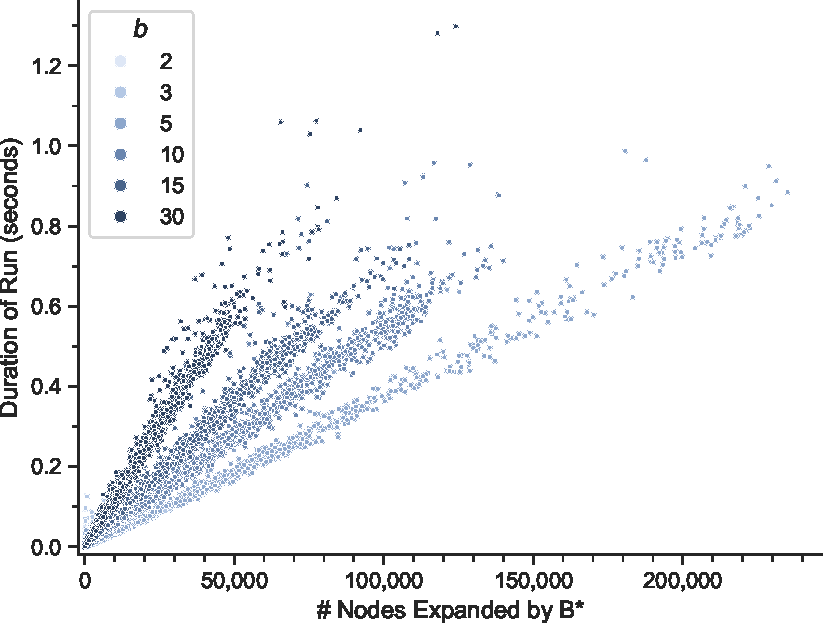
\includegraphics[scale=0.7]
	{figures/graphs/colour/fig1TimePerExpandedSolvedByAnyBstar.pdf}
	\fi
	\caption{This figure shows the duration of a run against the number of expansions for all runs solved by \textbf{B*} or \textbf{B*-alt}, from Experiment 1 (see Subsection \ref{subsec:ResultsExp1}). Runs displayed are categorised by the branching factor of the tree, which is negatively correlated with the number of expansions per second ($r\approx-0.54$).}
	\label{fig:Exp1TimePerExpandedSolvedByAnyBstar}
\end{figure}
%
\begin{figure}[htbp]
	\centering
	\ifMonochrome
	
\includegraphics[scale=0.7]
	{figures/graphs/monochrome/fig1TimePerExpandedSolvedByAnyBstarSQ.pdf}
	\else
	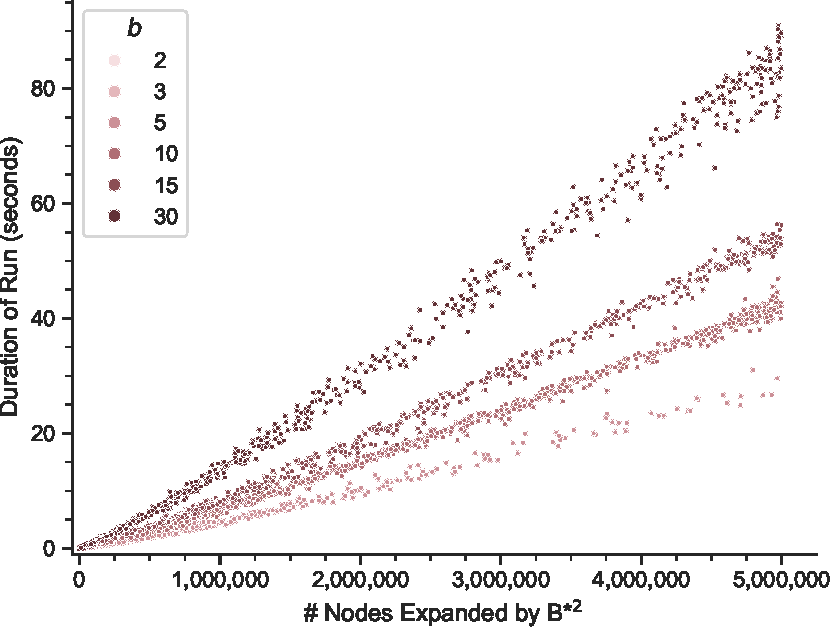
\includegraphics[scale=0.7]
	{figures/graphs/colour/fig1TimePerExpandedSolvedByAnyBstarSQ.pdf}
	\fi
	\caption{This figure shows the duration of a run against the number of expansions for all runs solved by \textbf{B*}$^2$ or \textbf{B*}$^2$\textbf{-alt}, for Experiment 1 (see Subsection \ref{subsec:ResultsExp1}). Runs displayed are categorised by the branching factor of the tree, which is negatively correlated with the number of expansions per second ($r\approx -0.62$).}
	\label{fig:Exp1TimePerExpandedSolvedByAnyBstarSQ}
\end{figure}
%
\begin{figure}[htbp]
	\centering
	\ifMonochrome
	
\includegraphics[scale=0.7]
	{figures/graphs/monochrome/fig1TimePerExpandedSolvedByAnyDfBstar.pdf}
	\else
	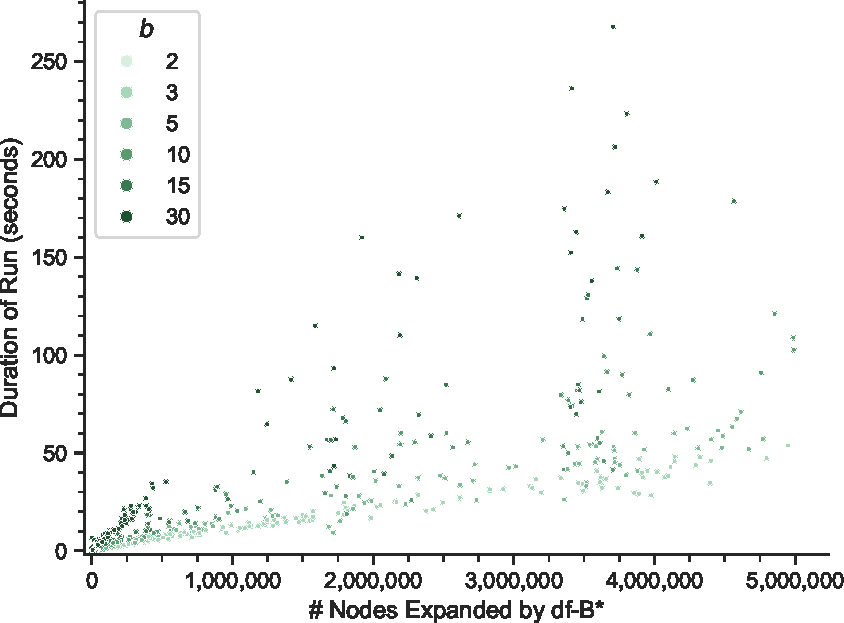
\includegraphics[scale=0.7]
	{figures/graphs/colour/fig1TimePerExpandedSolvedByAnyDfBstar.pdf}
	\fi
	\caption{This figure shows the duration of a run against the number of expansions for all runs solved by \textbf{df-B*} or \textbf{df-B*-alt}, for Experiment 1 (see Subsection \ref{subsec:ResultsExp1}). Runs displayed are categorised by the branching factor of the tree, which is not correlated with the number of expansions per second ($r\approx -0.03$).}
	\label{fig:Exp1TimePerExpandedSolvedByAnyDfBstar}
\end{figure}
\end{appendix}

\end{document}